\documentclass[a4paper,12pt]{article}
\usepackage{amsmath,amssymb,graphicx,setspace,float,enumitem,hyperref,xurl,geometry,fancyhdr,array,tabularx,multirow,booktabs,longtable,pdflscape,xcolor,caption,subcaption,tikz}
\usetikzlibrary{shapes,arrows.meta,positioning,calc,fit,backgrounds}
\geometry{top=2.7cm,bottom=2.2cm,left=1.5cm,right=1.5cm}
\setstretch{1.55}
\setlength{\parskip}{0.35em}
\setlength{\parindent}{0.8cm}
\setlength{\headheight}{24pt}
\Urlmuskip=0mu plus 1mu
\usepackage{xepersian}
\IfFontExistsTF{XB Niloofar}{\settextfont{XB Niloofar}\setdigitfont{XB Niloofar}}{\IfFontExistsTF{Amiri}{\settextfont{Amiri}\setdigitfont{Amiri}}{\settextfont{Noto Naskh Arabic}\setdigitfont{Noto Naskh Arabic}}}
\IfFontExistsTF{Times New Roman}{\setlatintextfont{Times New Roman}}{\setlatintextfont{DejaVu Serif}}
\hypersetup{unicode=true,breaklinks=true,colorlinks=true,linkcolor=blue!45!black,urlcolor=blue!45!black}
\newcommand{\NDCG}{\lr{NDCG@10}}
\newcommand{\MRR}{\lr{MRR@10}}
\newcommand{\Recall}{\lr{Recall@10}}
\newcolumntype{C}[1]{>{\centering\arraybackslash}m{#1}}
\newcolumntype{R}[1]{>{\raggedleft\arraybackslash}m{#1}}
\newcolumntype{L}[1]{>{\raggedright\arraybackslash}m{#1}}
\pagestyle{fancy}
\fancyhf{}
\fancyhead[R]{گزارش جامع آزمایش‌های \lr{ArguAna} و \lr{FiQA}}
\fancyhead[L]{\thepage}
\renewcommand{\headrulewidth}{0.4pt}

\begin{document}
\begin{titlepage}
\thispagestyle{empty}
\centering
\vspace*{1.6cm}
{\Large\bfseries باسمه تعالی\par}
\vspace{1.2cm}
{\Huge\bfseries گزارش جامع آزمایش‌های کاهش‌بُعد آگاه از نویز\par}
\vspace{0.6cm}
{\LARGE\bfseries روی مجموعه‌داده‌های \lr{ArguAna} و \lr{FiQA-2018}\par}
\vspace{1.5cm}
\begin{tabular}{|C{4.2cm}|C{5cm}|C{5cm}|}
\hline
\textbf{نام دانشجو} & \textbf{استاد راهنما} & \textbf{موضوع گزارش} \\
\hline
امیررضا تقدسی & دکتر هادی صدوقی یزدی & تحلیل جامع دو اجرای نهایی روش‌های ۱ تا ۱۹ \\
\hline
\end{tabular}
\vspace{1.6cm}
\begin{minipage}{0.88\textwidth}
\centering
این گزارش تمام خروجی‌های دو اجرای نهایی و اصلاح‌شده را پوشش می‌دهد: اجرای \lr{ArguAna} و اجرای \lr{FiQA-2018}. همه خطوط مبنا، روش‌های ۱ تا ۱۹، سه وضعیت ارزیابی، تحلیل خانواده‌ها، مطالعه حذف ترم‌ها، پایداری رتبه‌بندی، هندسه ماتریس‌ها، روند آموزش، هزینه حافظه و کنترل صحت ارزیاب در متن و پیوست‌ها گزارش شده‌اند.
\end{minipage}
\vfill
{\large گزارش فنی مستقل\par}
\end{titlepage}

\tableofcontents
\listoffigures
\listoftables
\newpage

\section{هدف و دامنه گزارش}
هدف این گزارش، ارائه تحلیل کامل و قابل بازتولید از دو آزمایش نهایی روی \lr{ArguAna} و \lr{FiQA-2018} است. پرسش‌های اصلی شامل امکان برتری نمایش ۱۲۸بعدی نویزآگاه بر بردار کامل ۳۸۴بعدی، مقایسه خانواده‌ها، نقش ترم‌های حذف نویز و حفظ سیگنال، پایداری فهرست بازیابی و صحت محاسبات است.

در هر دو اجرا، میانگین نویزی مستقیماً از دو ستون واقعی نویز تایپی و نویز مشابه \lr{OCR} محاسبه شد. بیشینه اختلاف بازحساب با مقدار ذخیره‌شده برای \lr{ArguAna} برابر $1.11\times10^{-16}$ و برای \lr{FiQA} برابر $6.94\times10^{-17}$ بود.

\section{طراحی آزمایش}
\subsection{مجموعه‌داده‌ها و اندازه اجرا}
\begin{table}[H]
\centering
\caption{مشخصات دو اجرای نهایی}
\label{tab:datasets}
\begin{tabular}{|C{3cm}|C{2.5cm}|C{2.6cm}|C{2.6cm}|C{2.6cm}|}
\hline
\textbf{مجموعه‌داده} & \textbf{تعداد اسناد} & \textbf{کوئری ارزیابی‌شده} & \textbf{اسناد برازش} & \textbf{بُعد ورودی/خروجی} \\
\hline
\lr{ArguAna} & ۸۶۷۴ & ۱۴۰۱ & حداکثر ۴۰۰۰ & $384\rightarrow128$ \\
\hline
\lr{FiQA-2018} & ۵۷۶۳۸ & ۶۴۸ & حداکثر ۴۰۰۰ & $384\rightarrow128$ \\
\hline
\end{tabular}
\end{table}

در \lr{ArguAna} تعداد ۱۴۰۶ کوئری برای آمار نویز پردازش شد، اما ۱۴۰۱ کوئری دارای ارزیابی معتبر وارد محاسبه معیارها شدند. در \lr{FiQA} هر ۶۴۸ کوئری ارزیابی شد.

\subsection{مدل تعبیه و پروتکل برازش}
مدل تعبیه در هر دو آزمایش \lr{sentence-transformers/all-MiniLM-L6-v2} با بُعد ۳۸۴ بود. همه روش‌ها روی اسناد پیکره برازش شدند. کوئری‌های آزمون، نسخه‌های نویزی کوئری‌ها و برچسب‌های ارتباط وارد آموزش نشدند؛ بنابراین نشت کوئری یا \lr{qrels} وجود ندارد.

\subsection{شرایط نویزی}
فقط کوئری‌ها نویزی شدند و اسناد تمیز ماندند. شدت اسمی هر دو نویز $0.15$ و بذر نویز ۱۲۳۴ بود.
\begin{table}[H]
\centering
\caption{شدت واقعی نویز در کوئری‌ها}
\label{tab:noise-severity}
\begin{tabular}{|C{2.8cm}|C{2.8cm}|C{2.6cm}|C{2.6cm}|}
\hline
\textbf{مجموعه‌داده} & \textbf{نوع نویز} & \textbf{\lr{CER}} & \textbf{\lr{TER}} \\
\hline
\lr{ArguAna} & تایپی & \lr{0.1705} & \lr{0.6515} \\
\hline
\lr{ArguAna} & مشابه \lr{OCR} & \lr{0.0866} & \lr{0.3694} \\
\hline
\lr{FiQA} & تایپی & \lr{0.1739} & \lr{0.6374} \\
\hline
\lr{FiQA} & مشابه \lr{OCR} & \lr{0.0900} & \lr{0.3642} \\
\hline
\end{tabular}
\end{table}

\subsection{روش‌ها و خطوط مبنا}
در هر مجموعه‌داده ۲۳ حالت در سه وضعیت اجرا شد؛ بنابراین هر اجرا ۶۹ ردیف و مجموع دو اجرا ۱۳۸ ردیف نتیجه دارد.

\scriptsize
\begin{longtable}{|C{2.3cm}|C{5.3cm}|C{9.0cm}|}
\caption{روش‌ها و خطوط مبنای ارزیابی‌شده}\label{tab:methods}\\
\hline
\textbf{شناسه} & \textbf{خانواده} & \textbf{تعریف} \\
\hline
\endfirsthead
\hline
\textbf{شناسه} & \textbf{خانواده} & \textbf{تعریف} \\
\hline
\endhead
\lr{Full-384} & خط مبنا & بردار کامل ۳۸۴بعدی، بدون کاهش بُعد \\
\hline
\lr{PCA-128} & خط مبنا & کاهش بُعد با تحلیل مؤلفه‌های اصلی \\
\hline
\lr{SVD-128} & خط مبنا & کاهش بُعد با تجزیه مقدار منفرد \\
\hline
\lr{Random-128} & خط مبنا & فرافکنی تصادفی ۱۲۸بعدی \\
\hline
روش 1 & روش ۱ اصلی & نسخه اصلی گرادیانی با نویززدایی، ناوردایی، حذف نویز، حفظ سیگنال و متعامدسازی نرم/سخت \\
\hline
روش 2 & روش ۲ بسته & حل بسته نسبت سیگنال به نویز بر پایه مسئله مقدارویژه تعمیم‌یافته \\
\hline
روش 3 & روش ۳ مرز \lr{Top-k} & یادگیری مرز رتبه‌بندی \lr{Top-k} \\
\hline
روش 4 & روش ۱ با \lr{QR} اقلیدسی & روش ۱ با \lr{QR} اقلیدسی؛ مجموعه ترم‌ها: \lr{D+I+N+S} \\
\hline
روش 5 & روش ۱ با \lr{QR} اقلیدسی & روش ۱ با \lr{QR} اقلیدسی؛ مجموعه ترم‌ها: \lr{D+I+S} \\
\hline
روش 6 & روش ۱ با \lr{QR} اقلیدسی & روش ۱ با \lr{QR} اقلیدسی؛ مجموعه ترم‌ها: \lr{D+I+N} \\
\hline
روش 7 & روش ۱ با \lr{QR} اقلیدسی & روش ۱ با \lr{QR} اقلیدسی؛ مجموعه ترم‌ها: \lr{D+I} \\
\hline
روش 8 & مقداردهی روش ۲ و آموزش آزاد & مقداردهی روش ۲ و آموزش آزاد؛ پروژکتور عمومی؛ مجموعه ترم‌ها: \lr{D+I+N+S} \\
\hline
روش 9 & مقداردهی روش ۲ و آموزش آزاد & مقداردهی روش ۲ و آموزش آزاد؛ پروژکتور عمومی؛ مجموعه ترم‌ها: \lr{D+I+S} \\
\hline
روش 10 & مقداردهی روش ۲ و آموزش آزاد & مقداردهی روش ۲ و آموزش آزاد؛ پروژکتور عمومی؛ مجموعه ترم‌ها: \lr{D+I+N} \\
\hline
روش 11 & مقداردهی روش ۲ و آموزش آزاد & مقداردهی روش ۲ و آموزش آزاد؛ پروژکتور عمومی؛ مجموعه ترم‌ها: \lr{D+I} \\
\hline
روش 12 & مقداردهی روش ۲ و بازگردانی متریکی & مقداردهی روش ۲ و بازگردانی متریکی؛ پروژکتور عمومی؛ مجموعه ترم‌ها: \lr{D+I+N+S} \\
\hline
روش 13 & مقداردهی روش ۲ و بازگردانی متریکی & مقداردهی روش ۲ و بازگردانی متریکی؛ پروژکتور عمومی؛ مجموعه ترم‌ها: \lr{D+I+S} \\
\hline
روش 14 & مقداردهی روش ۲ و بازگردانی متریکی & مقداردهی روش ۲ و بازگردانی متریکی؛ پروژکتور عمومی؛ مجموعه ترم‌ها: \lr{D+I+N} \\
\hline
روش 15 & مقداردهی روش ۲ و بازگردانی متریکی & مقداردهی روش ۲ و بازگردانی متریکی؛ پروژکتور عمومی؛ مجموعه ترم‌ها: \lr{D+I} \\
\hline
روش 16 & \lr{QR} خروجی روش ۲ و سپس روش ۱ & \lr{QR} خروجی روش ۲ و سپس روش ۱؛ مجموعه ترم‌ها: \lr{D+I+N+S} \\
\hline
روش 17 & \lr{QR} خروجی روش ۲ و سپس روش ۱ & \lr{QR} خروجی روش ۲ و سپس روش ۱؛ مجموعه ترم‌ها: \lr{D+I+S} \\
\hline
روش 18 & \lr{QR} خروجی روش ۲ و سپس روش ۱ & \lr{QR} خروجی روش ۲ و سپس روش ۱؛ مجموعه ترم‌ها: \lr{D+I+N} \\
\hline
روش 19 & \lr{QR} خروجی روش ۲ و سپس روش ۱ & \lr{QR} خروجی روش ۲ و سپس روش ۱؛ مجموعه ترم‌ها: \lr{D+I} \\
\hline
\end{longtable}

\subsection{تنظیمات آموزش و ارزیابی}
روش‌های گرادیانی ۱۰ دوره با اندازه دسته ۲۵۶ اجرا شدند. وزن‌های روش ۱ برابر $\lambda_D=1$، $\lambda_I=0.5$، $\lambda_N=0.3$، $\lambda_S=0.1$ و $\lambda_O=0.001$ بود. روش ۲ از ۴۰۰۰ بردار تمیز و ۱۶۰۰۰ اختلاف نویزی استفاده کرد.

معیارهای \lr{NDCG}، \lr{MRR}، \lr{Recall}، \lr{Precision}، \lr{MAP} و \lr{Hit Rate} در برش‌های ۱، ۵، ۱۰ و ۲۰ محاسبه شدند. ارزیاب اصلی \lr{pytrec\_eval} بود و اختلاف آن با ارزیاب داخلی برای همه معیارها و برش‌ها صفر ثبت شد.

\section{نتایج کامل \lr{ArguAna}}
\subsection{جدول جامع}
\begin{landscape}
\scriptsize
\begin{longtable}{|C{2.6cm}|C{2cm}|C{2cm}|C{2cm}|C{2.1cm}|C{2.1cm}|C{2.1cm}|C{2.2cm}|}
\caption{خلاصه کامل نتایج اصلی روی ArguAna}\label{tab:arg-summary}\\
\hline
\textbf{روش} & \textbf{تمیز NDCG} & \textbf{تایپی NDCG} & \textbf{OCR NDCG} & \textbf{میانگین نویزی} & \textbf{بدترین نویز} & \textbf{میانگین MRR} & \textbf{میانگین Recall} \\
\hline
\endfirsthead
\hline
\textbf{روش} & \textbf{تمیز NDCG} & \textbf{تایپی NDCG} & \textbf{OCR NDCG} & \textbf{میانگین نویزی} & \textbf{بدترین نویز} & \textbf{میانگین MRR} & \textbf{میانگین Recall} \\
\hline
\endhead
\lr{Full-384} & \lr{0.3711} & \lr{0.1911} & \lr{0.2865} & \lr{0.2388} & \lr{0.1911} & \lr{0.1546} & \lr{0.5103} \\
\hline
\lr{PCA-128} & \lr{0.3621} & \lr{0.1771} & \lr{0.2727} & \lr{0.2249} & \lr{0.1771} & \lr{0.1472} & \lr{0.4761} \\
\hline
\lr{SVD-128} & \lr{0.3661} & \lr{0.1850} & \lr{0.2813} & \lr{0.2332} & \lr{0.1850} & \lr{0.1511} & \lr{0.4989} \\
\hline
\lr{Random-128} & \lr{0.3423} & \lr{0.1137} & \lr{0.2157} & \lr{0.1647} & \lr{0.1137} & \lr{0.1068} & \lr{0.3537} \\
\hline
روش 1 & \lr{0.3539} & \lr{0.1897} & \lr{0.2702} & \lr{0.2300} & \lr{0.1897} & \lr{0.1505} & \lr{0.4861} \\
\hline
روش 2 & \lr{0.3708} & \lr{0.2394} & \lr{0.3118} & \lr{0.2756} & \lr{0.2394} & \textbf{\lr{0.1808}} & \lr{0.5796} \\
\hline
روش 3 & \lr{0.3640} & \lr{0.2195} & \lr{0.2980} & \lr{0.2588} & \lr{0.2195} & \lr{0.1687} & \lr{0.5485} \\
\hline
روش 4 & \lr{0.3544} & \lr{0.1905} & \lr{0.2710} & \lr{0.2307} & \lr{0.1905} & \lr{0.1508} & \lr{0.4886} \\
\hline
روش 5 & \lr{0.3531} & \lr{0.1894} & \lr{0.2696} & \lr{0.2295} & \lr{0.1894} & \lr{0.1503} & \lr{0.4847} \\
\hline
روش 6 & \lr{0.3540} & \lr{0.1906} & \lr{0.2694} & \lr{0.2300} & \lr{0.1906} & \lr{0.1508} & \lr{0.4854} \\
\hline
روش 7 & \lr{0.3529} & \lr{0.1892} & \lr{0.2698} & \lr{0.2295} & \lr{0.1892} & \lr{0.1504} & \lr{0.4843} \\
\hline
روش 8 & \lr{0.3705} & \lr{0.2393} & \textbf{\lr{0.3132}} & \textbf{\lr{0.2762}} & \lr{0.2393} & \lr{0.1797} & \lr{0.5864} \\
\hline
روش 9 & \lr{0.3697} & \lr{0.2315} & \lr{0.3120} & \lr{0.2718} & \lr{0.2315} & \lr{0.1765} & \lr{0.5785} \\
\hline
روش 10 & \textbf{\lr{0.3715}} & \textbf{\lr{0.2395}} & \lr{0.3124} & \lr{0.2759} & \textbf{\lr{0.2395}} & \lr{0.1792} & \textbf{\lr{0.5871}} \\
\hline
روش 11 & \lr{0.3703} & \lr{0.2311} & \lr{0.3105} & \lr{0.2708} & \lr{0.2311} & \lr{0.1757} & \lr{0.5767} \\
\hline
روش 12 & \lr{0.3708} & \lr{0.2380} & \lr{0.3122} & \lr{0.2751} & \lr{0.2380} & \lr{0.1793} & \lr{0.5828} \\
\hline
روش 13 & \lr{0.3699} & \lr{0.2317} & \lr{0.3105} & \lr{0.2711} & \lr{0.2317} & \lr{0.1764} & \lr{0.5757} \\
\hline
روش 14 & \lr{0.3708} & \lr{0.2386} & \lr{0.3118} & \lr{0.2752} & \lr{0.2386} & \lr{0.1792} & \lr{0.5839} \\
\hline
روش 15 & \lr{0.3704} & \lr{0.2308} & \lr{0.3103} & \lr{0.2706} & \lr{0.2308} & \lr{0.1761} & \lr{0.5746} \\
\hline
روش 16 & \lr{0.3635} & \lr{0.2245} & \lr{0.2989} & \lr{0.2617} & \lr{0.2245} & \lr{0.1714} & \lr{0.5521} \\
\hline
روش 17 & \lr{0.3639} & \lr{0.2253} & \lr{0.2990} & \lr{0.2621} & \lr{0.2253} & \lr{0.1716} & \lr{0.5535} \\
\hline
روش 18 & \lr{0.3642} & \lr{0.2255} & \lr{0.3002} & \lr{0.2629} & \lr{0.2255} & \lr{0.1723} & \lr{0.5542} \\
\hline
روش 19 & \lr{0.3641} & \lr{0.2256} & \lr{0.2999} & \lr{0.2627} & \lr{0.2256} & \lr{0.1721} & \lr{0.5546} \\
\hline
\end{longtable}
\end{landscape}
\begin{figure}[H]
\centering
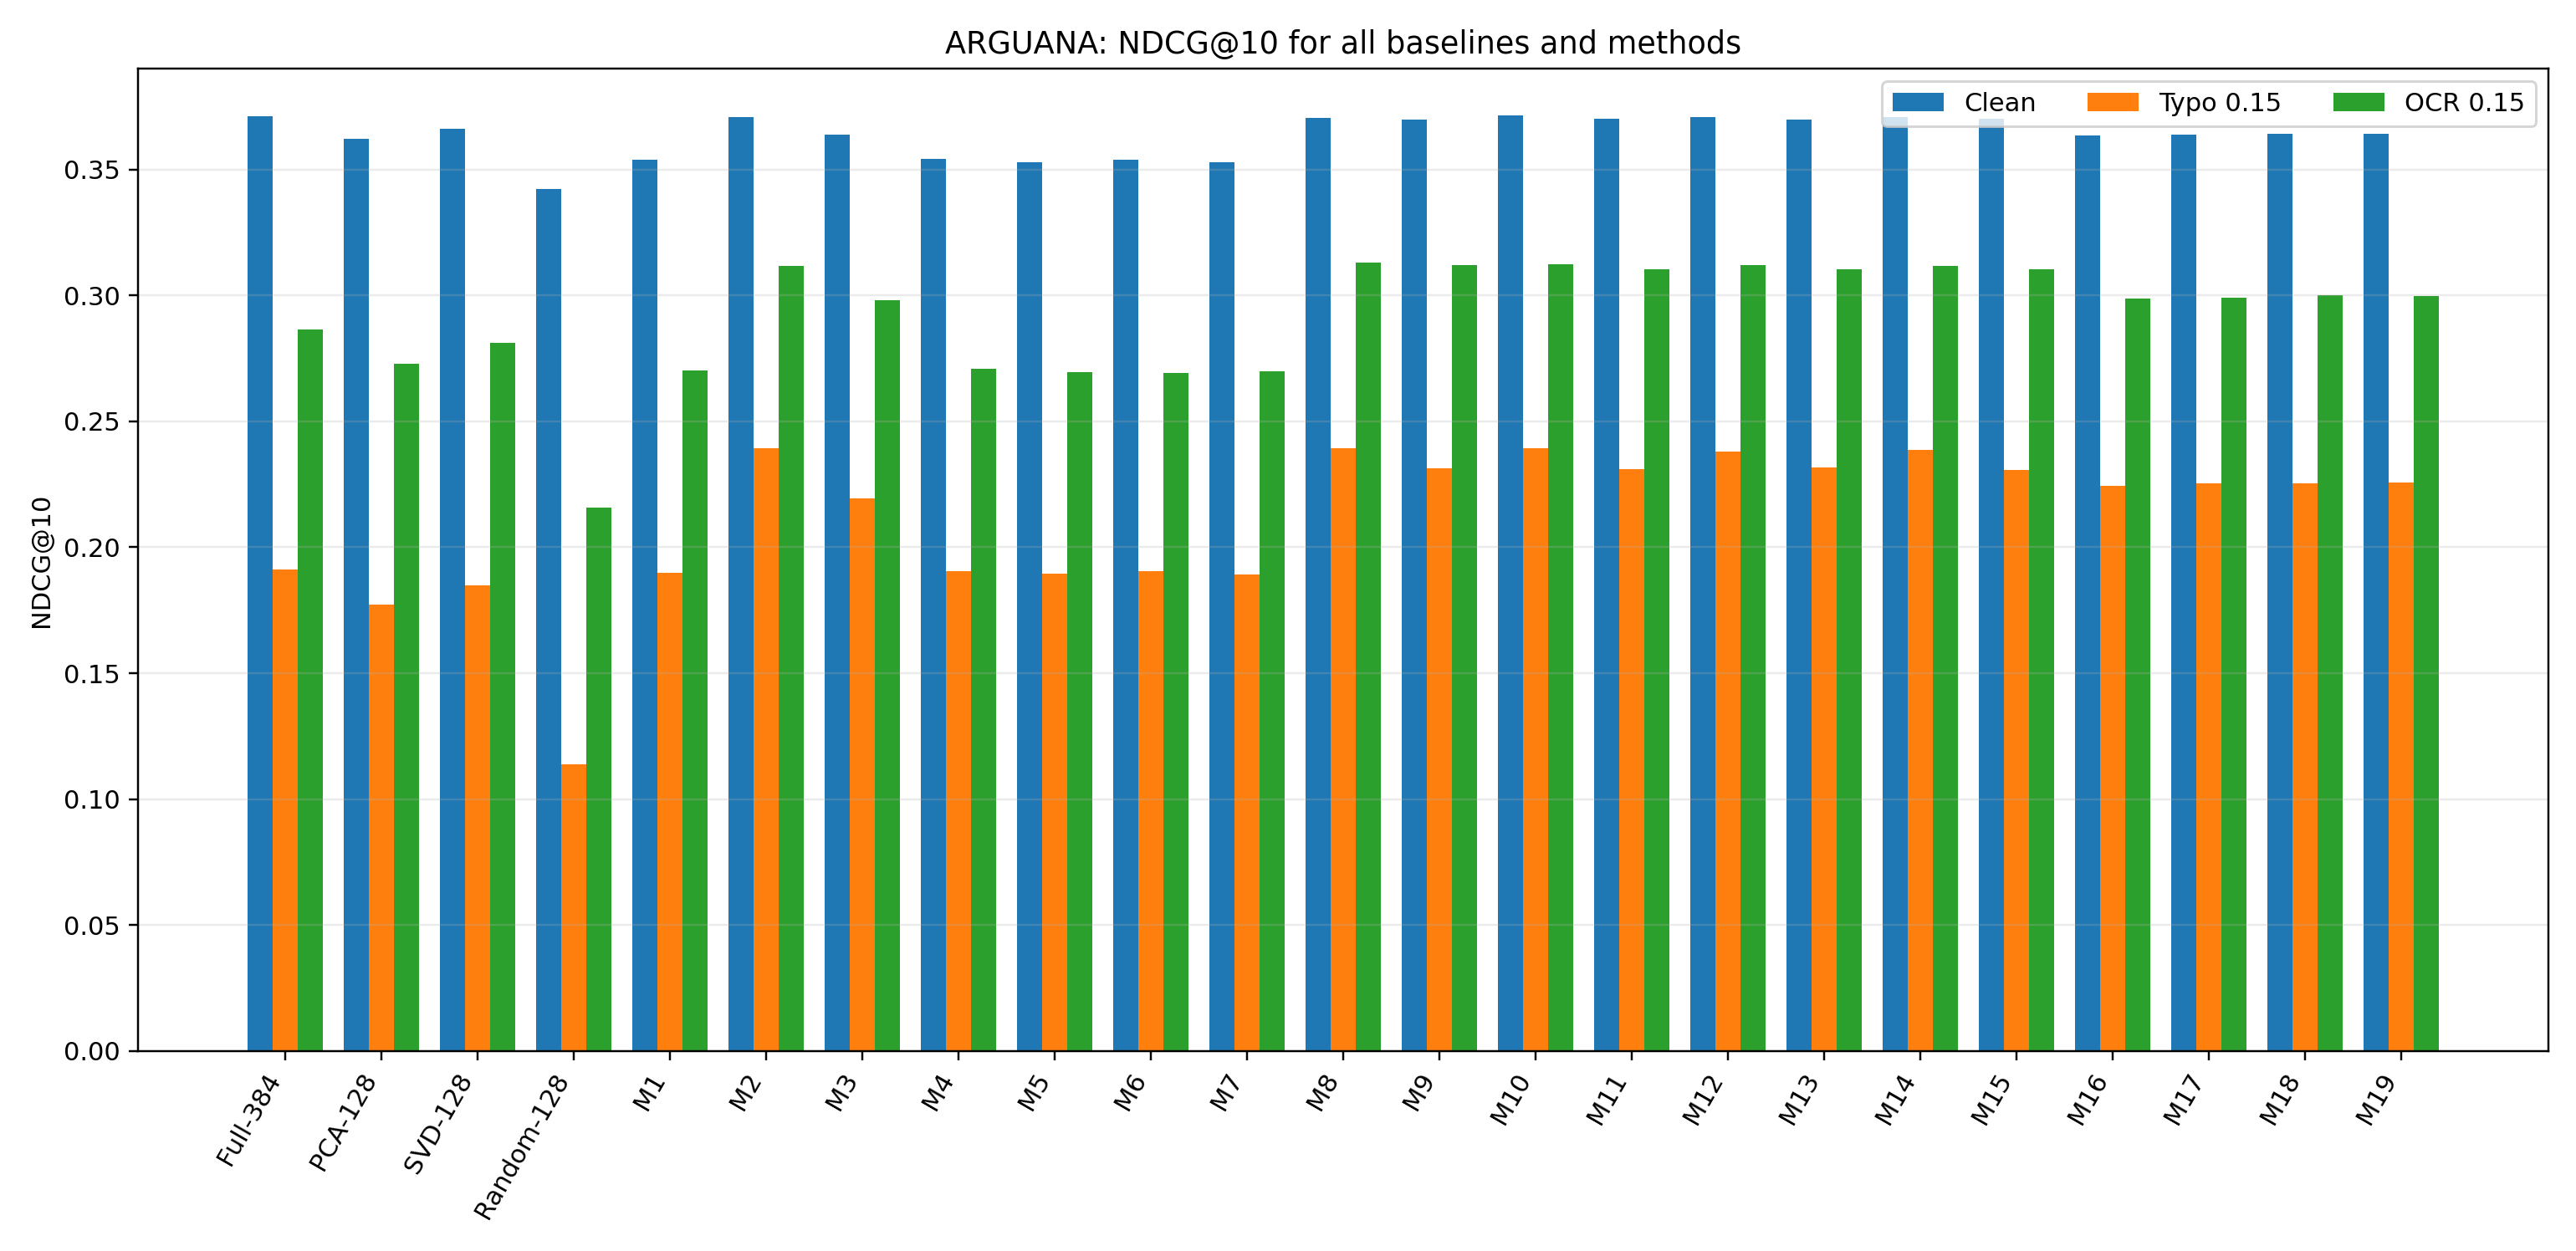
\includegraphics[width=\textwidth]{figures/arguana_all_ndcg.png}
\caption{مقایسه \lr{NDCG@10} تمیز، نویز تایپی و نویز مشابه \lr{OCR} برای همه روش‌ها در \lr{ArguAna}}
\end{figure}

\subsection{تحلیل حالت تمیز}
بردار کامل \NDCG برابر \lr{0.371061} داشت. روش ۱۰ با \lr{0.371516} بهترین \NDCG و \MRR تمیز را ثبت کرد؛ بهبود آن تنها \lr{0.123\%} بود. بردار کامل همچنان بهترین \Recall، \lr{Hit@10}، \lr{NDCG@20} و \lr{Recall@20} را داشت.

\subsection{تحلیل نویز تایپی}
بردار کامل به \lr{0.191102} افت کرد. روش ۱۰ با \lr{0.239457} بهترین شد و \lr{25.30\%} بهتر از بردار کامل بود. روش ۲ با \lr{0.239447} عملاً برابر بود و بهترین \MRR تایپی را ثبت کرد. چهارده روش از ۱۹ روش پروژه از بردار کامل عبور کردند.

\subsection{تحلیل نویز مشابه \lr{OCR}}
روش ۸ با \lr{0.313170} بهترین شد و نسبت به بردار کامل با مقدار \lr{0.286474}، \lr{9.32\%} بهبود داشت. روش ۲ بهترین \MRR و روش ۸ بهترین \Recall را ثبت کرد.

\subsection{میانگین نویزی و نرخ حفظ عملکرد}
روش ۸ با میانگین \lr{0.276213} بهترین شد؛ روش ۱۰ و روش ۲ به‌ترتیب \lr{0.275919} و \lr{0.275635} داشتند. روش ۸ نسبت به بردار کامل \lr{15.67\%} بهتر بود. نرخ حفظ عملکرد از \lr{64.35\%} برای بردار کامل به \lr{74.55\%} برای روش ۸ رسید.

\subsection{مقایسه خانواده‌ها}
\scriptsize
\begin{longtable}{|C{5cm}|C{2cm}|C{2.4cm}|C{2.4cm}|C{2.4cm}|C{2.4cm}|}
\caption{مقایسه خانواده‌ها روی ArguAna}\label{tab:arg-family}\\
\hline
\textbf{خانواده} & \textbf{تعداد روش} & \textbf{میانگین تمیز} & \textbf{میانگین نویزی} & \textbf{بهترین عضو} & \textbf{بدترین حالت} \\
\hline
\endfirsthead
\hline
\textbf{خانواده} & \textbf{تعداد روش} & \textbf{میانگین تمیز} & \textbf{میانگین نویزی} & \textbf{بهترین عضو} & \textbf{بدترین حالت} \\
\hline
\endhead
روش ۱ با \lr{QR} اقلیدسی & 4 & \lr{0.3536} & \lr{0.2300} & \lr{0.2307} & \lr{0.1906} \\
\hline
مقداردهی روش ۲ و آموزش آزاد & 4 & \lr{0.3705} & \lr{0.2737} & \lr{0.2762} & \lr{0.2395} \\
\hline
مقداردهی روش ۲ و بازگردانی متریکی & 4 & \lr{0.3705} & \lr{0.2730} & \lr{0.2752} & \lr{0.2386} \\
\hline
\lr{QR} خروجی روش ۲ و سپس روش ۱ & 4 & \lr{0.3639} & \lr{0.2624} & \lr{0.2629} & \lr{0.2256} \\
\hline
\end{longtable}
خانواده آزاد اول و خانواده متریکی با فاصله بسیار کم دوم شد. خانواده \lr{QR} خروجی روش ۲ و خانواده روش ۱ به‌ترتیب در رتبه‌های بعدی قرار گرفتند.

\subsection{مطالعه حذف ترم‌ها}
\scriptsize
\begin{longtable}{|C{5.5cm}|C{2.4cm}|C{2.4cm}|C{2.4cm}|C{2.6cm}|}
\caption{میانگین NDCG نویزی در مطالعه حذف ترم‌ها روی ArguAna}\label{tab:arg-ablation}\\
\hline
\textbf{خانواده} & \textbf{فقط پایه} & \textbf{کامل} & \textbf{بدون حذف نویز} & \textbf{بدون حفظ سیگنال} \\
\hline
\endfirsthead
\hline
\textbf{خانواده} & \textbf{فقط پایه} & \textbf{کامل} & \textbf{بدون حذف نویز} & \textbf{بدون حفظ سیگنال} \\
\hline
\endhead
روش ۱ با \lr{QR} اقلیدسی & \lr{0.2295} & \textbf{\lr{0.2307}} & \lr{0.2295} & \lr{0.2300} \\
\hline
مقداردهی روش ۲ و آموزش آزاد & \lr{0.2708} & \textbf{\lr{0.2762}} & \lr{0.2718} & \lr{0.2759} \\
\hline
مقداردهی روش ۲ و بازگردانی متریکی & \lr{0.2706} & \lr{0.2751} & \lr{0.2711} & \textbf{\lr{0.2752}} \\
\hline
\lr{QR} خروجی روش ۲ و سپس روش ۱ & \lr{0.2627} & \lr{0.2617} & \lr{0.2621} & \textbf{\lr{0.2629}} \\
\hline
\end{longtable}
حذف ترم حذف نویز در خانواده‌های آزاد و متریکی افت واضح ایجاد کرد، در حالی که حذف حفظ سیگنال تقریباً بدون هزینه بود. این نتیجه اهمیت ترم حذف نویز را نشان می‌دهد.

\subsection{پایداری فهرست بازیابی}
\begin{landscape}
\scriptsize
\begin{longtable}{|C{2cm}|C{2.3cm}|C{1.7cm}|C{2.2cm}|C{2.2cm}|C{2.2cm}|C{2.2cm}|C{2.5cm}|}
\caption{شاخص‌های پایداری روش‌های منتخب روی ArguAna}\label{tab:arg-robust}\\
\hline
\textbf{نویز} & \textbf{روش} & \textbf{NDCG} & \textbf{هم‌پوشانی ۲۰} & \textbf{ثبات رتبه اول} & \textbf{نرخ از دست‌رفتن} & \textbf{نرخ به‌دست‌آوردن} & \textbf{جابجایی رتبه مرتبط} \\
\hline
\endfirsthead
\hline
\textbf{نویز} & \textbf{روش} & \textbf{NDCG} & \textbf{هم‌پوشانی ۲۰} & \textbf{ثبات رتبه اول} & \textbf{نرخ از دست‌رفتن} & \textbf{نرخ به‌دست‌آوردن} & \textbf{جابجایی رتبه مرتبط} \\
\hline
\endhead
تایپی & \lr{Full-384} & \lr{0.1911} & \lr{0.3093} & \lr{0.5853} & \lr{0.3640} & \lr{0.0178} & \lr{6.856} \\
\hline
تایپی & روش ۲ & \lr{0.2394} & \lr{0.3912} & \lr{0.7173} & \lr{0.2641} & \lr{0.0257} & \lr{4.962} \\
\hline
تایپی & روش ۸ & \lr{0.2393} & \lr{0.3990} & \lr{0.7323} & \lr{0.2577} & \lr{0.0278} & \lr{4.902} \\
\hline
تایپی & روش ۱۰ & \lr{0.2395} & \lr{0.3985} & \lr{0.7323} & \lr{0.2562} & \lr{0.0264} & \lr{4.959} \\
\hline
تایپی & روش ۱۲ & \lr{0.2380} & \lr{0.3980} & \lr{0.7338} & \lr{0.2570} & \lr{0.0271} & \lr{4.965} \\
\hline
تایپی & روش ۱۴ & \lr{0.2386} & \lr{0.3993} & \lr{0.7323} & \lr{0.2570} & \lr{0.0278} & \lr{4.961} \\
\hline
مشابه OCR & \lr{Full-384} & \lr{0.2865} & \lr{0.4977} & \lr{0.8979} & \lr{0.1685} & \lr{0.0178} & \lr{3.165} \\
\hline
مشابه OCR & روش ۲ & \lr{0.3118} & \lr{0.5763} & \lr{0.9350} & \lr{0.1049} & \lr{0.0257} & \lr{1.954} \\
\hline
مشابه OCR & روش ۸ & \lr{0.3132} & \lr{0.5809} & \lr{0.9400} & \lr{0.1006} & \lr{0.0228} & \lr{1.943} \\
\hline
مشابه OCR & روش ۱۰ & \lr{0.3124} & \lr{0.5820} & \lr{0.9400} & \lr{0.1021} & \lr{0.0228} & \lr{1.992} \\
\hline
مشابه OCR & روش ۱۲ & \lr{0.3122} & \lr{0.5811} & \lr{0.9372} & \lr{0.1064} & \lr{0.0243} & \lr{1.995} \\
\hline
مشابه OCR & روش ۱۴ & \lr{0.3118} & \lr{0.5815} & \lr{0.9393} & \lr{0.1064} & \lr{0.0243} & \lr{2.006} \\
\hline
\end{longtable}
\end{landscape}
در نویز تایپی، هم‌پوشانی ۲۰ نتیجه بردار کامل $0.3093$ و نرخ از دست‌رفتن hit برابر $0.3640$ بود. روش‌های ۸ تا ۱۴ هم‌پوشانی را به حدود $0.399$ و نرخ از دست‌رفتن را به حدود $0.256$ رساندند. در نویز مشابه \lr{OCR} نیز همان الگو تکرار شد.

\subsection{هندسه و آموزش}
خانواده‌های روش ۱ و \lr{QR} نرم نزدیک $\sqrt{128}$ و عدد شرط نزدیک ۱ داشتند. خانواده‌های آزاد و متریکی از نظر اقلیدسی غیرمتعامد بودند، اما خانواده متریکی خطای متریکی را به حدود $0.03$ تا $0.06$ محدود کرد. ترم حذف نویز خام در خانواده‌های مقداردهی‌شده با روش ۲ از نظر عددی غالب شد، ولی retrieval همچنان قوی باقی ماند.

\section{نتایج کامل \lr{FiQA-2018}}
\subsection{جدول جامع}
\begin{landscape}
\scriptsize
\begin{longtable}{|C{2.6cm}|C{2cm}|C{2cm}|C{2cm}|C{2.1cm}|C{2.1cm}|C{2.1cm}|C{2.2cm}|}
\caption{خلاصه کامل نتایج اصلی روی FiQA-2018}\label{tab:fiqa-summary}\\
\hline
\textbf{روش} & \textbf{تمیز NDCG} & \textbf{تایپی NDCG} & \textbf{OCR NDCG} & \textbf{میانگین نویزی} & \textbf{بدترین نویز} & \textbf{میانگین MRR} & \textbf{میانگین Recall} \\
\hline
\endfirsthead
\hline
\textbf{روش} & \textbf{تمیز NDCG} & \textbf{تایپی NDCG} & \textbf{OCR NDCG} & \textbf{میانگین نویزی} & \textbf{بدترین نویز} & \textbf{میانگین MRR} & \textbf{میانگین Recall} \\
\hline
\endhead
\lr{Full-384} & \textbf{\lr{0.3687}} & \lr{0.0678} & \textbf{\lr{0.1756}} & \lr{0.1217} & \lr{0.0678} & \lr{0.1470} & \lr{0.1618} \\
\hline
\lr{PCA-128} & \lr{0.3358} & \lr{0.0448} & \lr{0.1493} & \lr{0.0970} & \lr{0.0448} & \lr{0.1176} & \lr{0.1323} \\
\hline
\lr{SVD-128} & \lr{0.3375} & \lr{0.0491} & \lr{0.1519} & \lr{0.1005} & \lr{0.0491} & \lr{0.1239} & \lr{0.1365} \\
\hline
\lr{Random-128} & \lr{0.2941} & \lr{0.0381} & \lr{0.1111} & \lr{0.0746} & \lr{0.0381} & \lr{0.0902} & \lr{0.1013} \\
\hline
روش 1 & \lr{0.3049} & \lr{0.0476} & \lr{0.1417} & \lr{0.0946} & \lr{0.0476} & \lr{0.1216} & \lr{0.1251} \\
\hline
روش 2 & \lr{0.3256} & \lr{0.0774} & \lr{0.1681} & \lr{0.1227} & \lr{0.0774} & \lr{0.1543} & \lr{0.1605} \\
\hline
روش 3 & \lr{0.3373} & \lr{0.0649} & \lr{0.1589} & \lr{0.1119} & \lr{0.0649} & \lr{0.1381} & \lr{0.1488} \\
\hline
روش 4 & \lr{0.3044} & \lr{0.0472} & \lr{0.1415} & \lr{0.0943} & \lr{0.0472} & \lr{0.1201} & \lr{0.1251} \\
\hline
روش 5 & \lr{0.3044} & \lr{0.0465} & \lr{0.1423} & \lr{0.0944} & \lr{0.0465} & \lr{0.1205} & \lr{0.1249} \\
\hline
روش 6 & \lr{0.3045} & \lr{0.0453} & \lr{0.1394} & \lr{0.0923} & \lr{0.0453} & \lr{0.1178} & \lr{0.1229} \\
\hline
روش 7 & \lr{0.3042} & \lr{0.0456} & \lr{0.1400} & \lr{0.0928} & \lr{0.0456} & \lr{0.1180} & \lr{0.1243} \\
\hline
روش 8 & \lr{0.3250} & \lr{0.0787} & \lr{0.1698} & \lr{0.1242} & \lr{0.0787} & \lr{0.1561} & \lr{0.1639} \\
\hline
روش 9 & \lr{0.3256} & \lr{0.0792} & \lr{0.1689} & \lr{0.1240} & \lr{0.0792} & \lr{0.1562} & \lr{0.1636} \\
\hline
روش 10 & \lr{0.3243} & \lr{0.0793} & \lr{0.1689} & \lr{0.1241} & \lr{0.0793} & \lr{0.1559} & \lr{0.1633} \\
\hline
روش 11 & \lr{0.3244} & \lr{0.0802} & \lr{0.1682} & \lr{0.1242} & \lr{0.0802} & \textbf{\lr{0.1566}} & \lr{0.1632} \\
\hline
روش 12 & \lr{0.3235} & \lr{0.0796} & \lr{0.1698} & \textbf{\lr{0.1247}} & \lr{0.0796} & \lr{0.1563} & \lr{0.1642} \\
\hline
روش 13 & \lr{0.3231} & \lr{0.0807} & \lr{0.1664} & \lr{0.1236} & \lr{0.0807} & \lr{0.1554} & \lr{0.1620} \\
\hline
روش 14 & \lr{0.3231} & \lr{0.0800} & \lr{0.1687} & \lr{0.1244} & \lr{0.0800} & \lr{0.1555} & \textbf{\lr{0.1646}} \\
\hline
روش 15 & \lr{0.3235} & \textbf{\lr{0.0812}} & \lr{0.1668} & \lr{0.1240} & \textbf{\lr{0.0812}} & \lr{0.1554} & \lr{0.1637} \\
\hline
روش 16 & \lr{0.3220} & \lr{0.0608} & \lr{0.1635} & \lr{0.1122} & \lr{0.0608} & \lr{0.1439} & \lr{0.1440} \\
\hline
روش 17 & \lr{0.3234} & \lr{0.0611} & \lr{0.1640} & \lr{0.1126} & \lr{0.0611} & \lr{0.1444} & \lr{0.1442} \\
\hline
روش 18 & \lr{0.3214} & \lr{0.0612} & \lr{0.1616} & \lr{0.1114} & \lr{0.0612} & \lr{0.1427} & \lr{0.1433} \\
\hline
روش 19 & \lr{0.3219} & \lr{0.0613} & \lr{0.1631} & \lr{0.1122} & \lr{0.0613} & \lr{0.1442} & \lr{0.1440} \\
\hline
\end{longtable}
\end{landscape}
\begin{figure}[H]
\centering
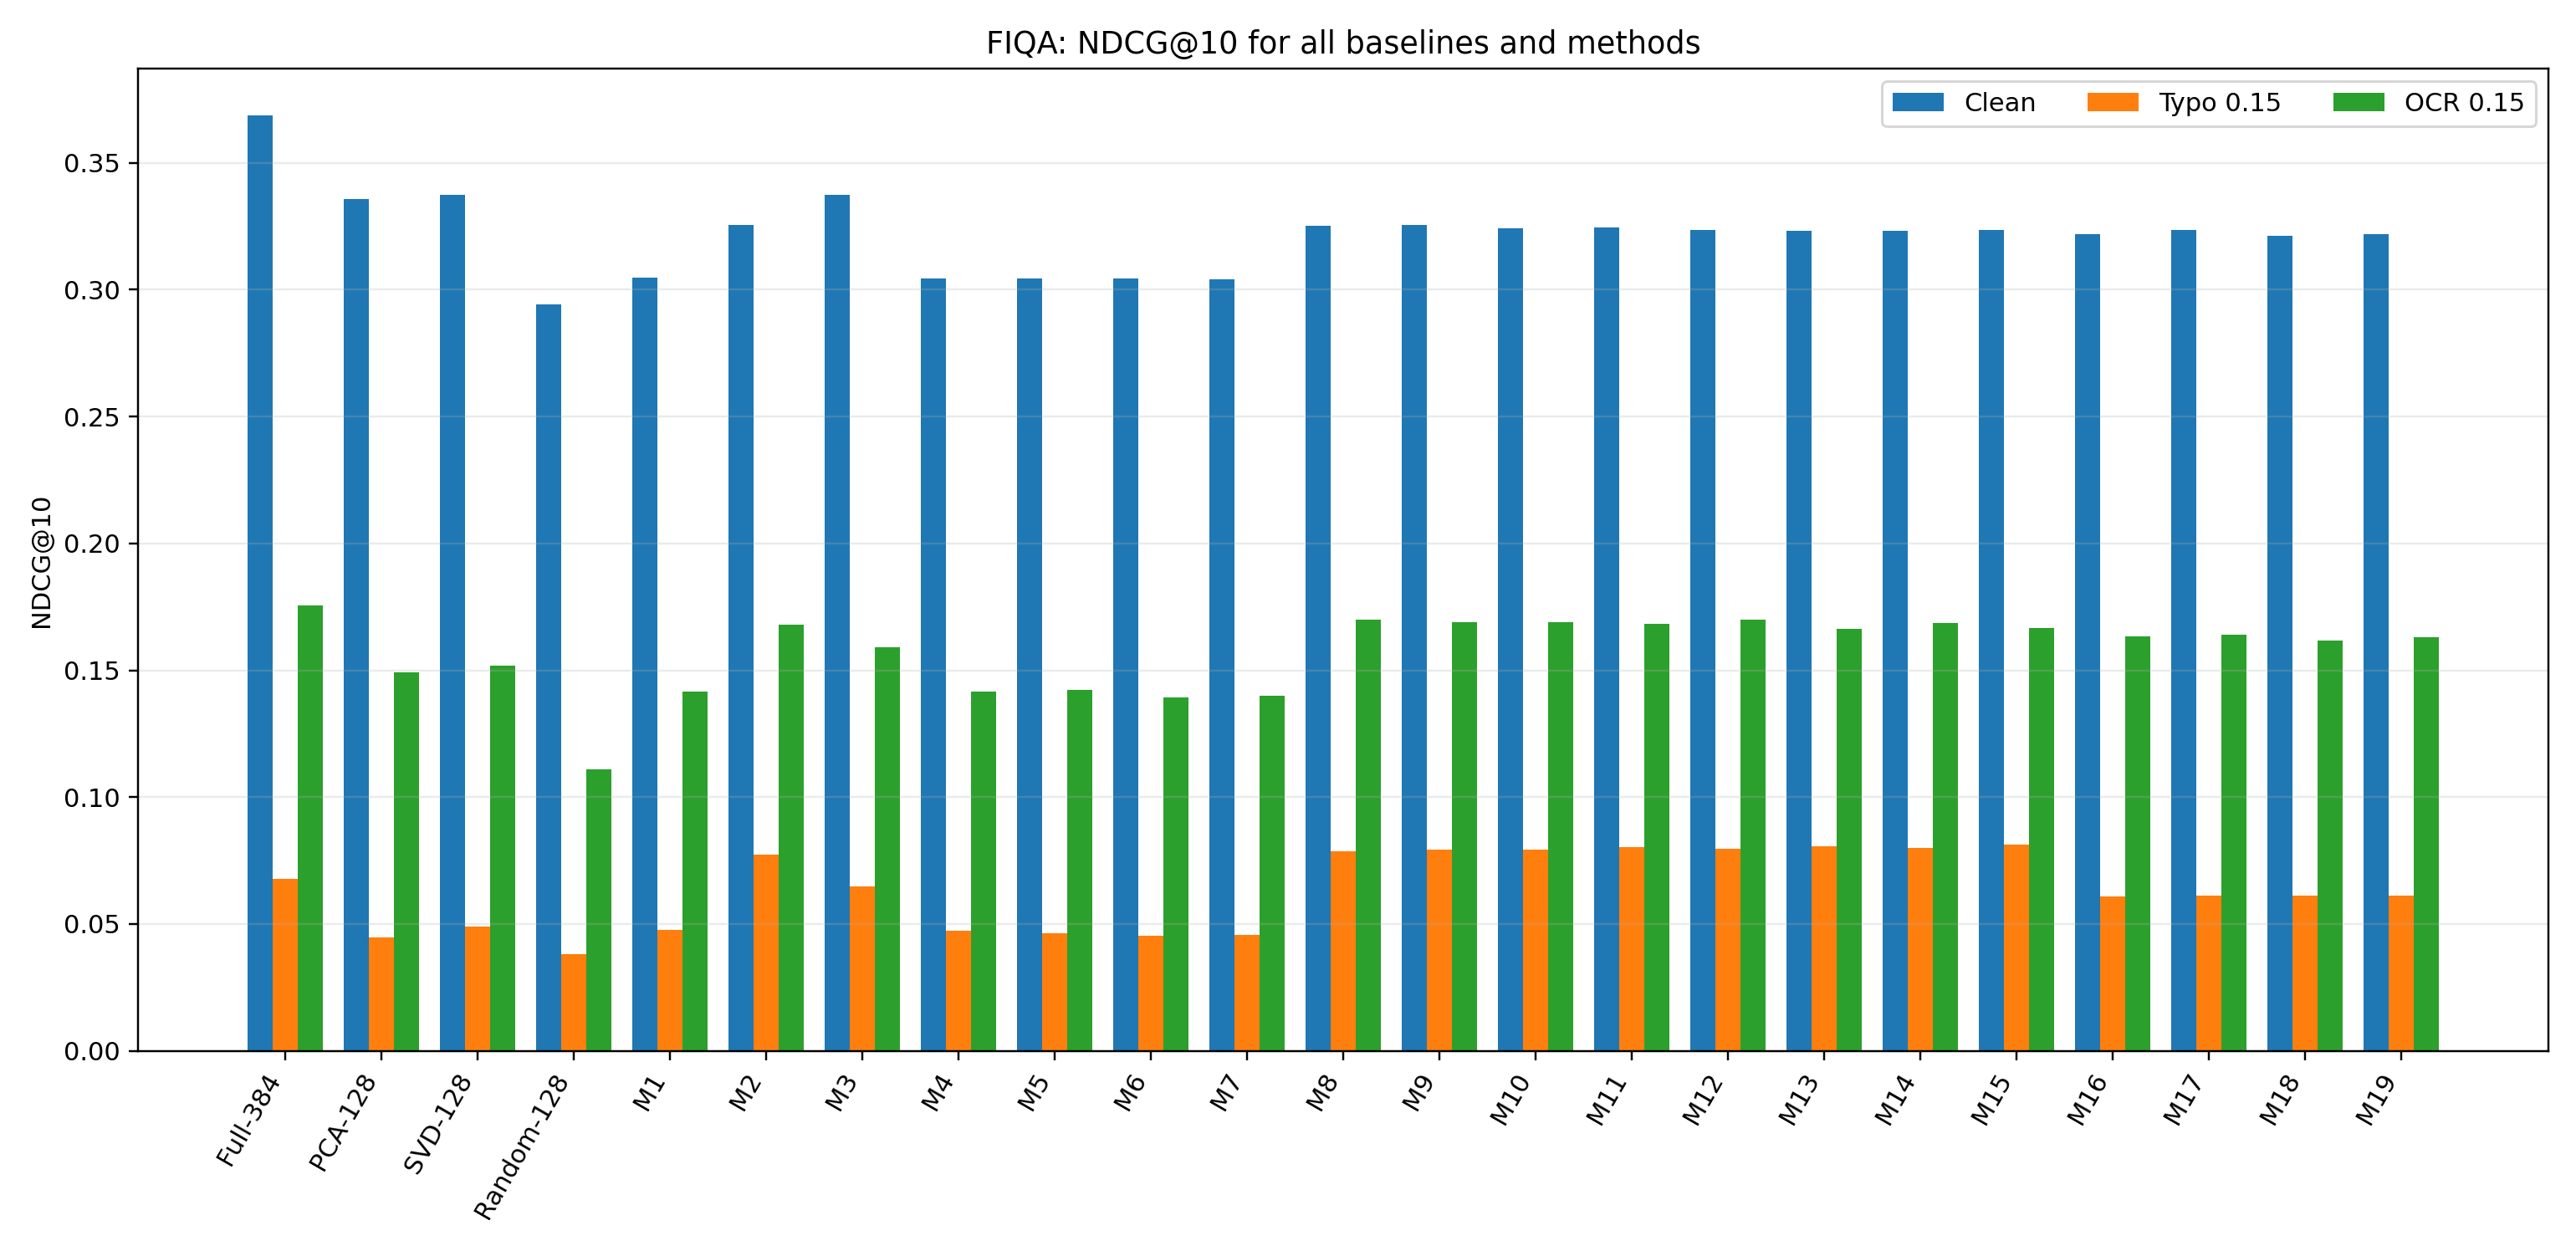
\includegraphics[width=\textwidth]{figures/fiqa_all_ndcg.png}
\caption{مقایسه \lr{NDCG@10} تمیز، نویز تایپی و نویز مشابه \lr{OCR} برای همه روش‌ها در \lr{FiQA}}
\end{figure}

\subsection{حالت تمیز}
بردار کامل با \lr{0.368671} بهترین بود. روش‌های مبتنی بر روش ۲ حدود ۱۱ تا ۱۲ درصد از کیفیت تمیز را از دست دادند؛ بنابراین کاهش بُعد در \lr{FiQA} هزینه تمیز محسوس داشت.

\subsection{نویز تایپی}
بردار کامل به \lr{0.067774} افت کرد. روش ۱۵ با \lr{0.081207} بهترین شد و \lr{19.82\%} بهبود ایجاد کرد. نه روش، شامل روش ۲ و اعضای خانواده‌های آزاد و متریکی، از بردار کامل بهتر شدند.

\subsection{نویز مشابه \lr{OCR}}
بردار کامل با \lr{0.175648} بهترین باقی ماند. روش ۱۲ با \lr{0.169826} بهترین روش پیشنهادی بود و \lr{-3.31\%} پایین‌تر از بردار کامل قرار گرفت. روش ۸ با وجود NDCG پایین‌تر، بهترین \MRR و \lr{Hit@10} را ثبت کرد.

\subsection{میانگین نویزی}
روش ۱۲ با \lr{0.124710} بهترین میانگین را ثبت کرد و \lr{2.46\%} از بردار کامل بهتر بود. این بهبود از نویز تایپی شدید ناشی شد. نرخ حفظ عملکرد از \lr{33.01\%} برای بردار کامل به \lr{38.54\%} برای روش ۱۲ افزایش یافت.

\subsection{مقایسه خانواده‌ها}
\scriptsize
\begin{longtable}{|C{5cm}|C{2cm}|C{2.4cm}|C{2.4cm}|C{2.4cm}|C{2.4cm}|}
\caption{مقایسه خانواده‌ها روی FiQA-2018}\label{tab:fiqa-family}\\
\hline
\textbf{خانواده} & \textbf{تعداد روش} & \textbf{میانگین تمیز} & \textbf{میانگین نویزی} & \textbf{بهترین عضو} & \textbf{بدترین حالت} \\
\hline
\endfirsthead
\hline
\textbf{خانواده} & \textbf{تعداد روش} & \textbf{میانگین تمیز} & \textbf{میانگین نویزی} & \textbf{بهترین عضو} & \textbf{بدترین حالت} \\
\hline
\endhead
روش ۱ با \lr{QR} اقلیدسی & 4 & \lr{0.3044} & \lr{0.0935} & \lr{0.0944} & \lr{0.0472} \\
\hline
مقداردهی روش ۲ و آموزش آزاد & 4 & \lr{0.3248} & \lr{0.1241} & \lr{0.1242} & \lr{0.0802} \\
\hline
مقداردهی روش ۲ و بازگردانی متریکی & 4 & \lr{0.3233} & \lr{0.1242} & \lr{0.1247} & \lr{0.0812} \\
\hline
\lr{QR} خروجی روش ۲ و سپس روش ۱ & 4 & \lr{0.3222} & \lr{0.1121} & \lr{0.1126} & \lr{0.0613} \\
\hline
\end{longtable}
خانواده متریکی با اختلاف $0.000025$ از خانواده آزاد جلو افتاد؛ این فاصله در یک اجرای تک‌بذر معنی‌دار نیست، اما نشان می‌دهد حفظ هندسه متریکی در برخی دامنه‌ها می‌تواند مفید باشد.

\subsection{مطالعه حذف ترم‌ها}
\scriptsize
\begin{longtable}{|C{5.5cm}|C{2.4cm}|C{2.4cm}|C{2.4cm}|C{2.6cm}|}
\caption{میانگین NDCG نویزی در مطالعه حذف ترم‌ها روی FiQA-2018}\label{tab:fiqa-ablation}\\
\hline
\textbf{خانواده} & \textbf{فقط پایه} & \textbf{کامل} & \textbf{بدون حذف نویز} & \textbf{بدون حفظ سیگنال} \\
\hline
\endfirsthead
\hline
\textbf{خانواده} & \textbf{فقط پایه} & \textbf{کامل} & \textbf{بدون حذف نویز} & \textbf{بدون حفظ سیگنال} \\
\hline
\endhead
روش ۱ با \lr{QR} اقلیدسی & \lr{0.0928} & \lr{0.0943} & \textbf{\lr{0.0944}} & \lr{0.0923} \\
\hline
مقداردهی روش ۲ و آموزش آزاد & \lr{0.1242} & \textbf{\lr{0.1242}} & \lr{0.1240} & \lr{0.1241} \\
\hline
مقداردهی روش ۲ و بازگردانی متریکی & \lr{0.1240} & \textbf{\lr{0.1247}} & \lr{0.1236} & \lr{0.1244} \\
\hline
\lr{QR} خروجی روش ۲ و سپس روش ۱ & \lr{0.1122} & \lr{0.1122} & \textbf{\lr{0.1126}} & \lr{0.1114} \\
\hline
\end{longtable}
در خانواده متریکی نسخه کامل بهترین بود. در خانواده آزاد چهار نسخه بسیار نزدیک بودند. اثر ترم‌ها به هندسه خانواده وابسته است.

\subsection{پایداری فهرست}
\begin{landscape}
\scriptsize
\begin{longtable}{|C{2cm}|C{2.3cm}|C{1.7cm}|C{2.2cm}|C{2.2cm}|C{2.2cm}|C{2.2cm}|C{2.5cm}|}
\caption{شاخص‌های پایداری روش‌های منتخب روی FiQA-2018}\label{tab:fiqa-robust}\\
\hline
\textbf{نویز} & \textbf{روش} & \textbf{NDCG} & \textbf{هم‌پوشانی ۲۰} & \textbf{ثبات رتبه اول} & \textbf{نرخ از دست‌رفتن} & \textbf{نرخ به‌دست‌آوردن} & \textbf{جابجایی رتبه مرتبط} \\
\hline
\endfirsthead
\hline
\textbf{نویز} & \textbf{روش} & \textbf{NDCG} & \textbf{هم‌پوشانی ۲۰} & \textbf{ثبات رتبه اول} & \textbf{نرخ از دست‌رفتن} & \textbf{نرخ به‌دست‌آوردن} & \textbf{جابجایی رتبه مرتبط} \\
\hline
\endhead
تایپی & \lr{Full-384} & \lr{0.0678} & \lr{0.0835} & \lr{0.0694} & \lr{0.5278} & \lr{0.0108} & \lr{12.602} \\
\hline
تایپی & روش ۲ & \lr{0.0774} & \lr{0.1113} & \lr{0.1111} & \lr{0.4290} & \lr{0.0093} & \lr{11.549} \\
\hline
تایپی & روش ۸ & \lr{0.0787} & \lr{0.1133} & \lr{0.1034} & \lr{0.4228} & \lr{0.0077} & \lr{11.379} \\
\hline
تایپی & روش ۱۰ & \lr{0.0793} & \lr{0.1131} & \lr{0.1034} & \lr{0.4228} & \lr{0.0046} & \lr{11.342} \\
\hline
تایپی & روش ۱۲ & \lr{0.0796} & \lr{0.1126} & \lr{0.1034} & \lr{0.4244} & \lr{0.0077} & \lr{11.335} \\
\hline
تایپی & روش ۱۴ & \lr{0.0800} & \lr{0.1125} & \lr{0.1049} & \lr{0.4259} & \lr{0.0093} & \lr{11.284} \\
\hline
مشابه OCR & \lr{Full-384} & \lr{0.1756} & \lr{0.2471} & \lr{0.2747} & \lr{0.3133} & \lr{0.0185} & \lr{7.411} \\
\hline
مشابه OCR & روش ۲ & \lr{0.1681} & \lr{0.2823} & \lr{0.2994} & \lr{0.2593} & \lr{0.0247} & \lr{6.601} \\
\hline
مشابه OCR & روش ۸ & \lr{0.1698} & \lr{0.2836} & \lr{0.3009} & \lr{0.2608} & \lr{0.0231} & \lr{6.534} \\
\hline
مشابه OCR & روش ۱۰ & \lr{0.1689} & \lr{0.2834} & \lr{0.3040} & \lr{0.2670} & \lr{0.0201} & \lr{6.513} \\
\hline
مشابه OCR & روش ۱۲ & \lr{0.1698} & \lr{0.2821} & \lr{0.2978} & \lr{0.2639} & \lr{0.0247} & \lr{6.499} \\
\hline
مشابه OCR & روش ۱۴ & \lr{0.1687} & \lr{0.2828} & \lr{0.2978} & \lr{0.2685} & \lr{0.0247} & \lr{6.503} \\
\hline
\end{longtable}
\end{landscape}
روش‌های مبتنی بر روش ۲ در هر دو نویز هم‌پوشانی بیشتر و نرخ از دست‌رفتن کمتر از بردار کامل داشتند. با این حال در نویز \lr{OCR}، فهرست تمیز روش‌های کم‌بُعد از ابتدا ضعیف‌تر بود؛ بنابراین پایداری بهتر به برتری مطلق NDCG منجر نشد.

\section{تحلیل تطبیقی}
\begin{figure}[H]\centering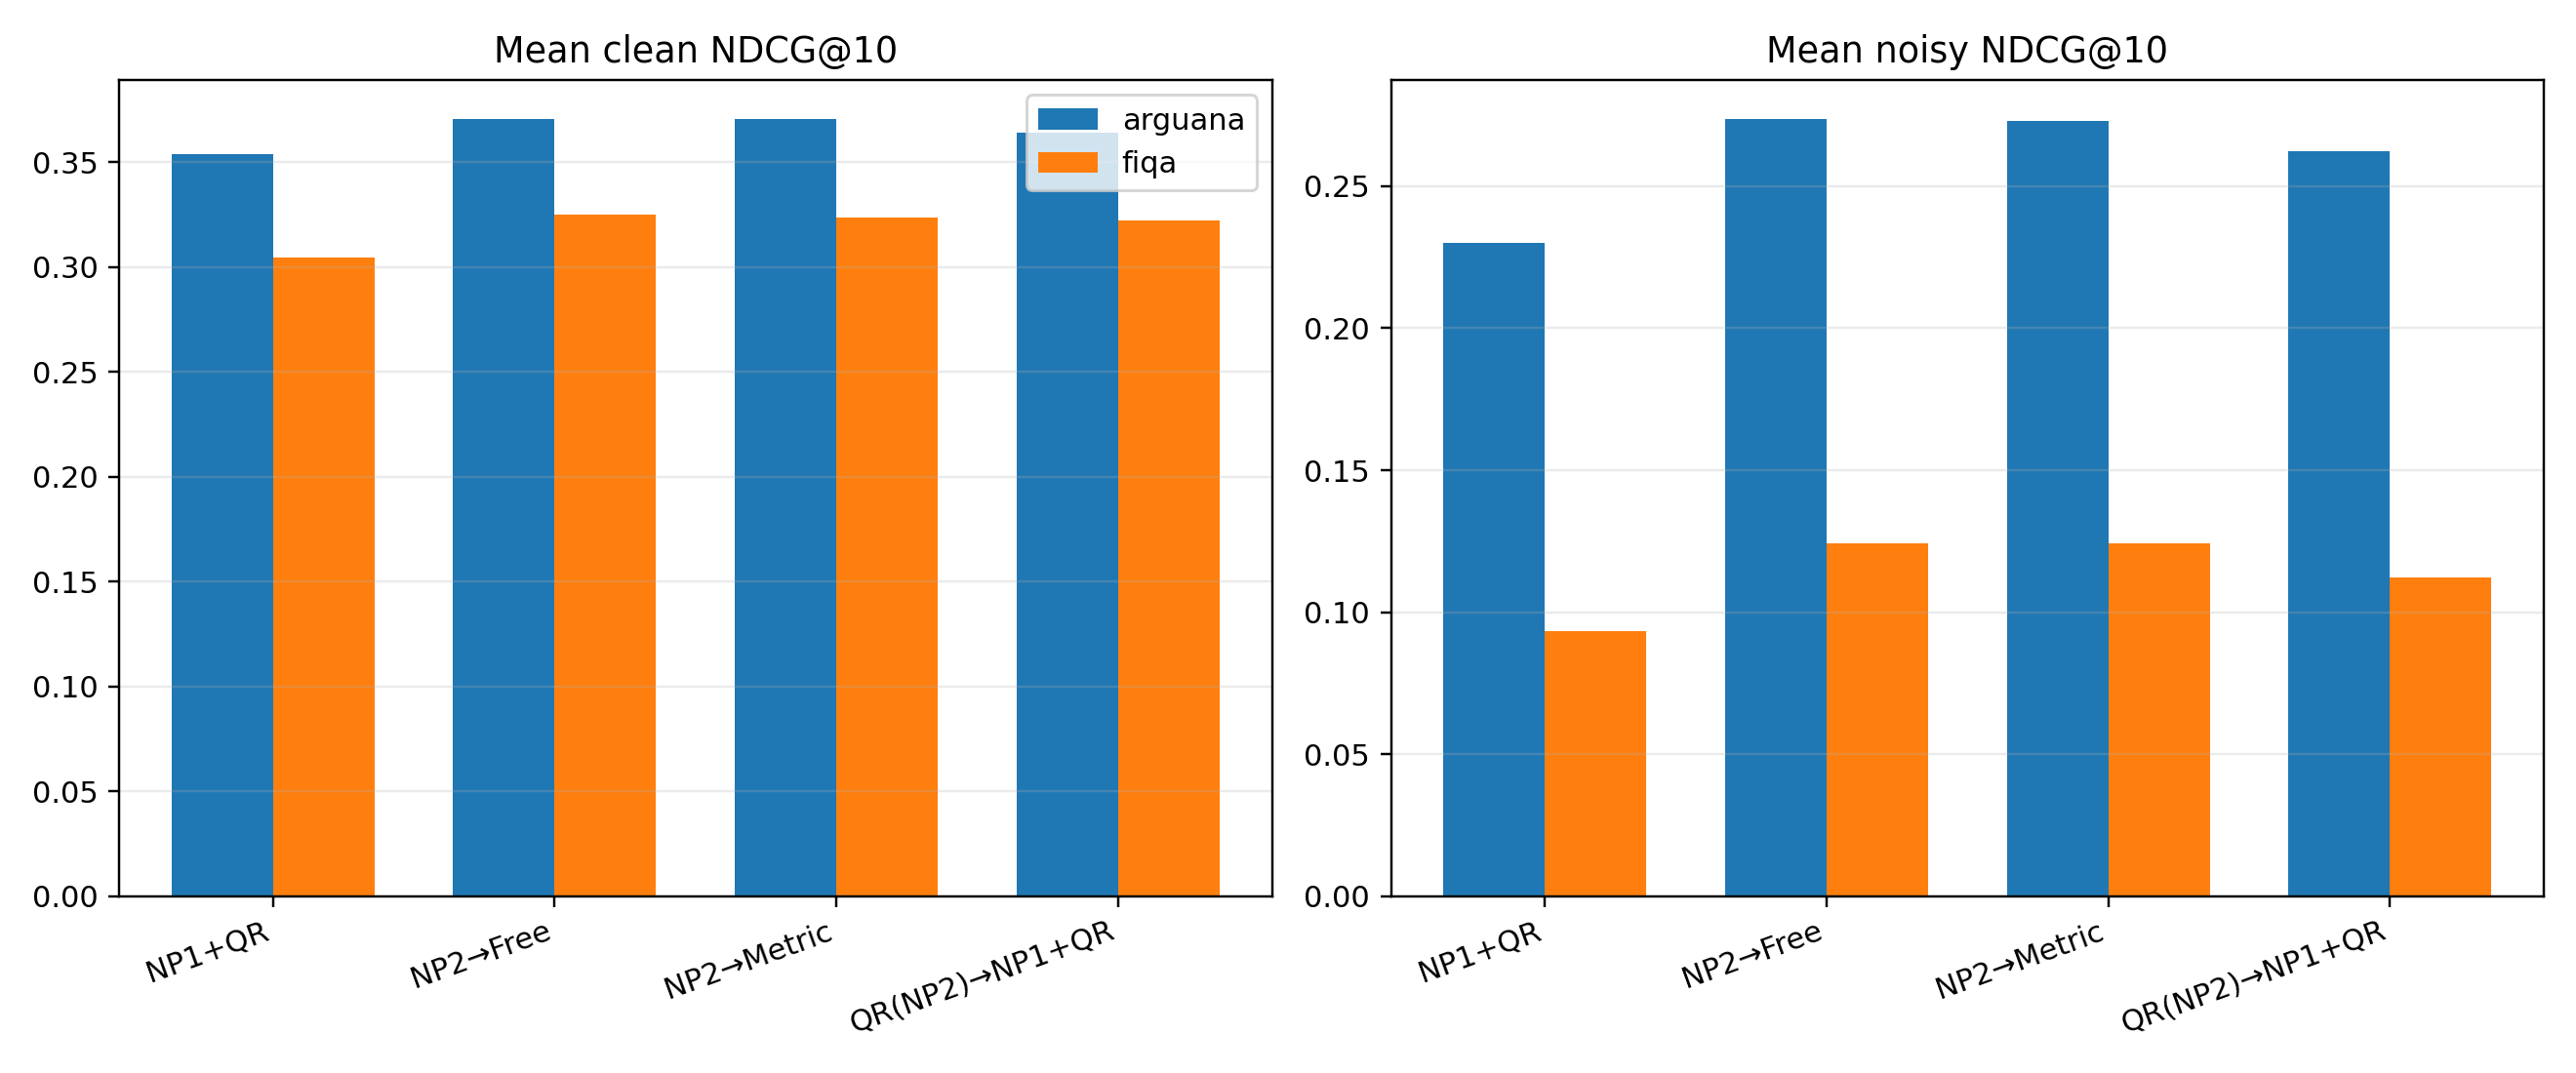
\includegraphics[width=\textwidth]{figures/family_comparison.png}\caption{میانگین تمیز و نویزی خانواده‌ها در دو مجموعه‌داده}\end{figure}
خانواده‌های آزاد و متریکی در هر دو دامنه بهترین گروه‌ها بودند. عامل مشترک موفقیت آن‌ها مقداردهی اولیه روش ۲ و استفاده از پروژکتور عمومی است.

\begin{figure}[H]\centering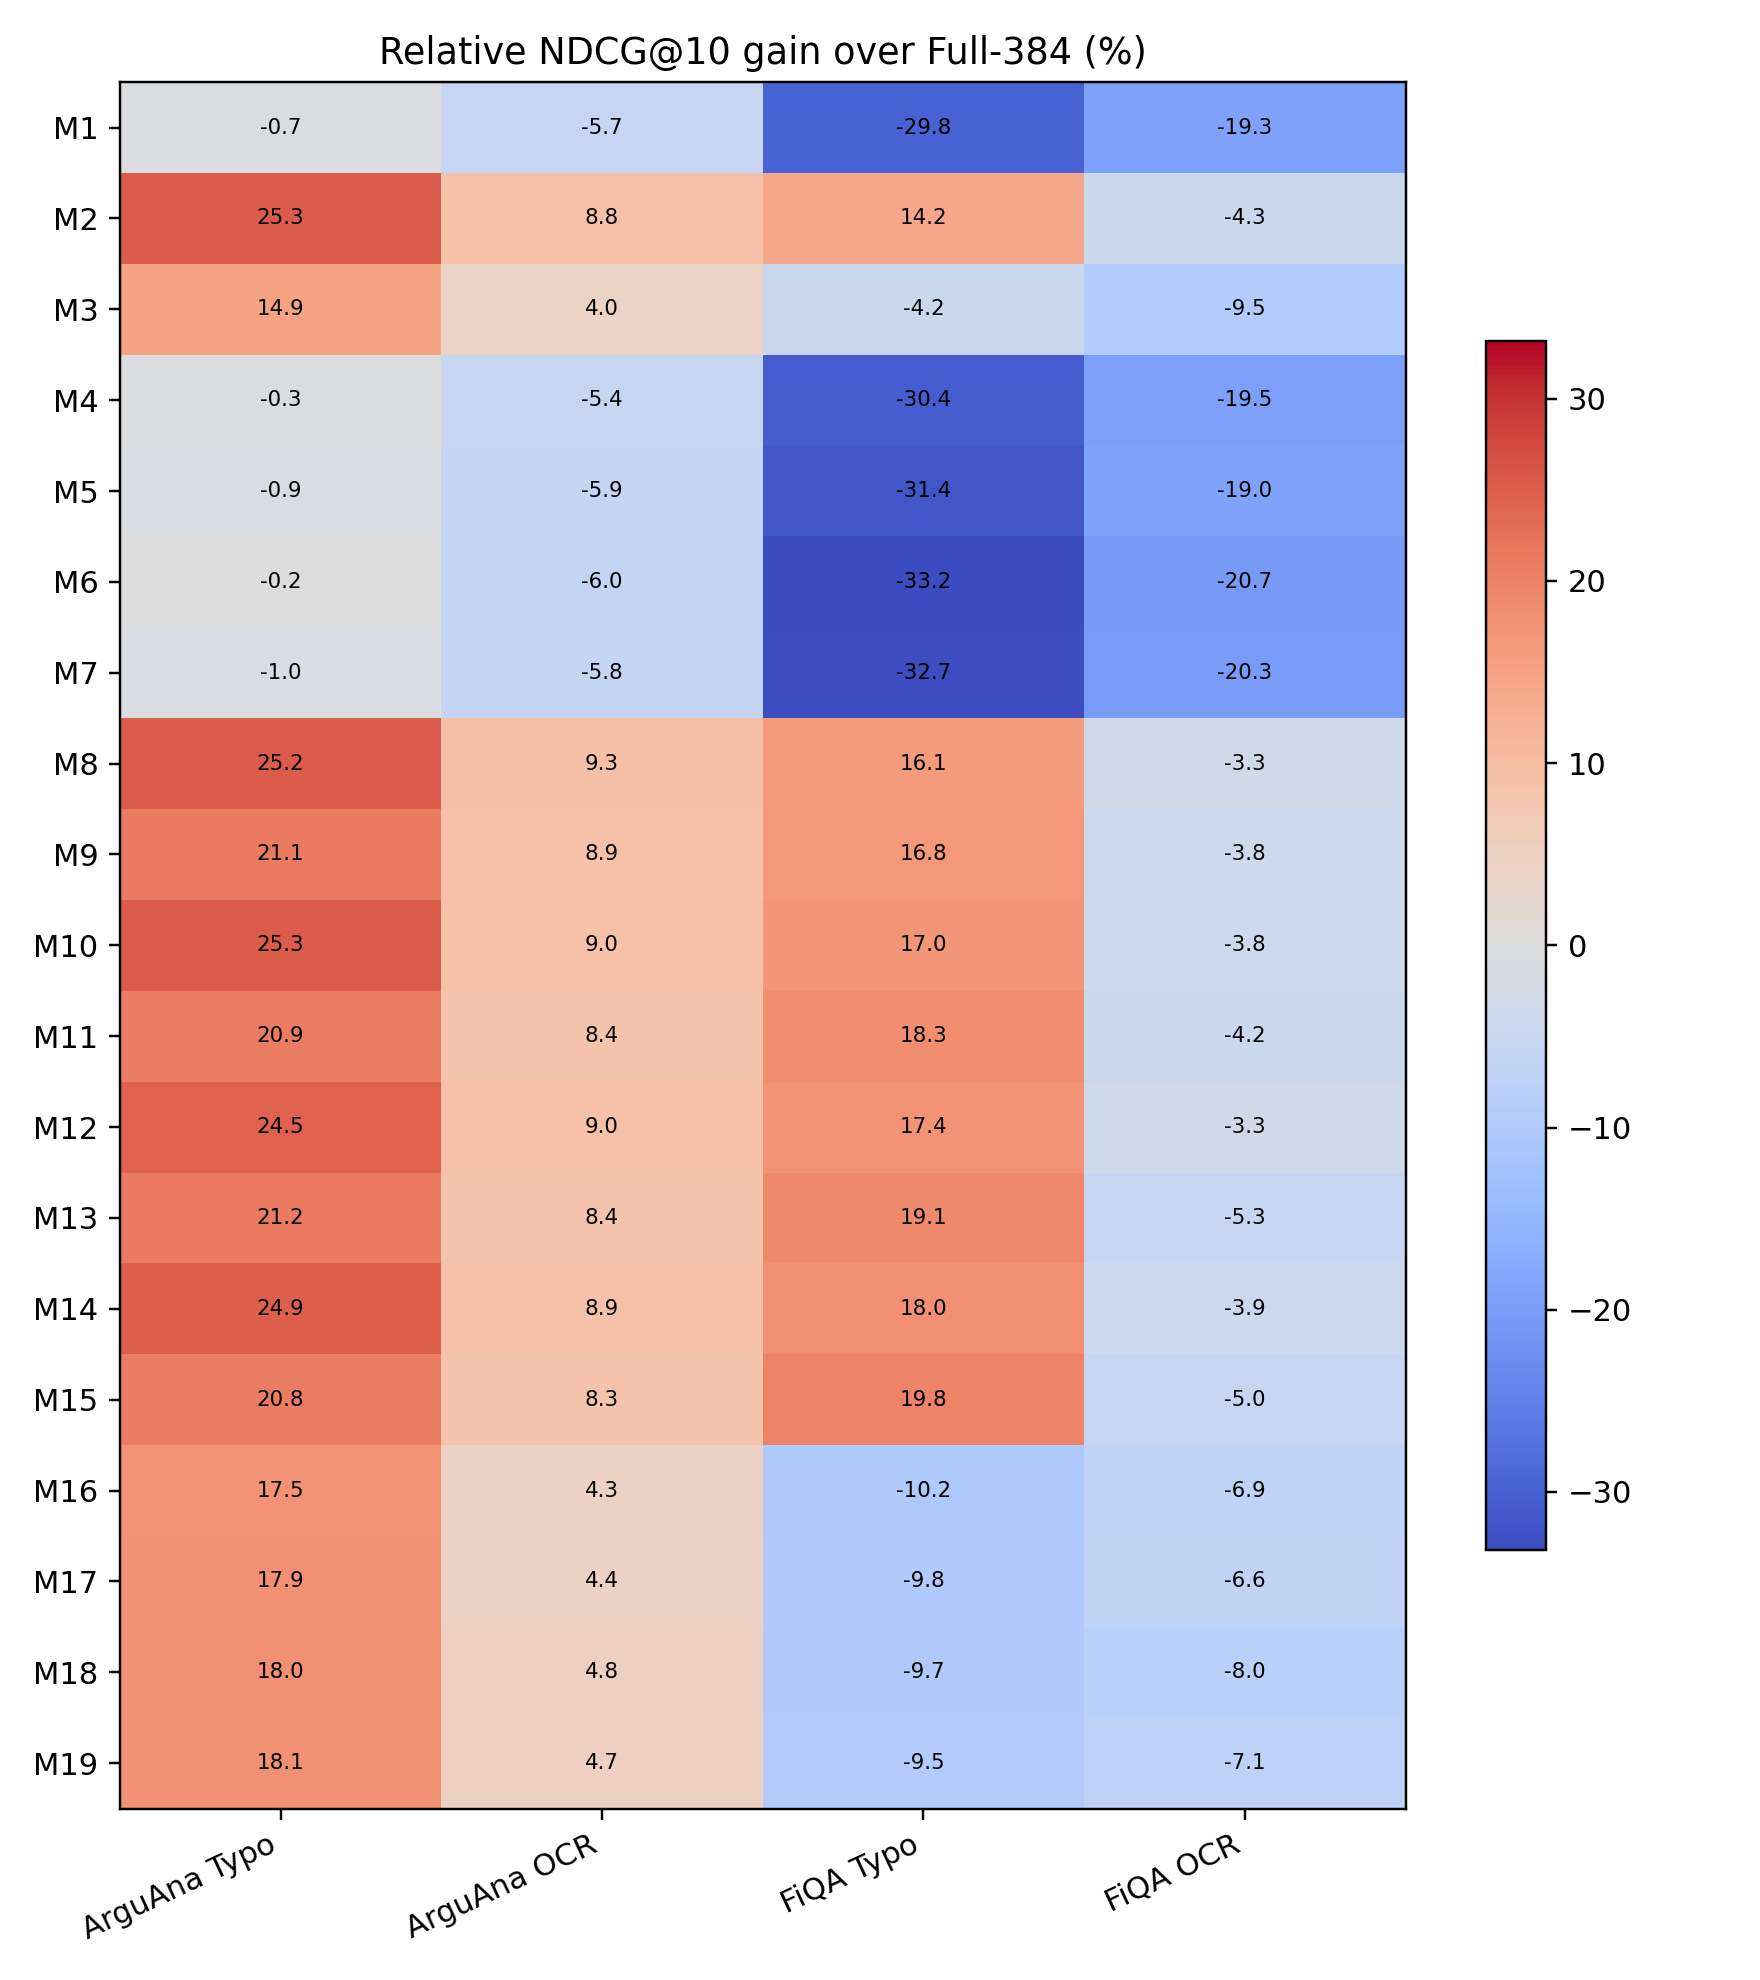
\includegraphics[width=0.82\textwidth]{figures/gain_heatmap.png}\caption{درصد تغییر NDCG@10 هر روش نسبت به بردار کامل در چهار حالت نویزی}\end{figure}
در \lr{ArguAna} چهارده روش در هر دو نویز بهتر شدند. در \lr{FiQA} نه روش فقط در نویز تایپی و میانگین نویزی بهتر بودند.

\begin{figure}[H]\centering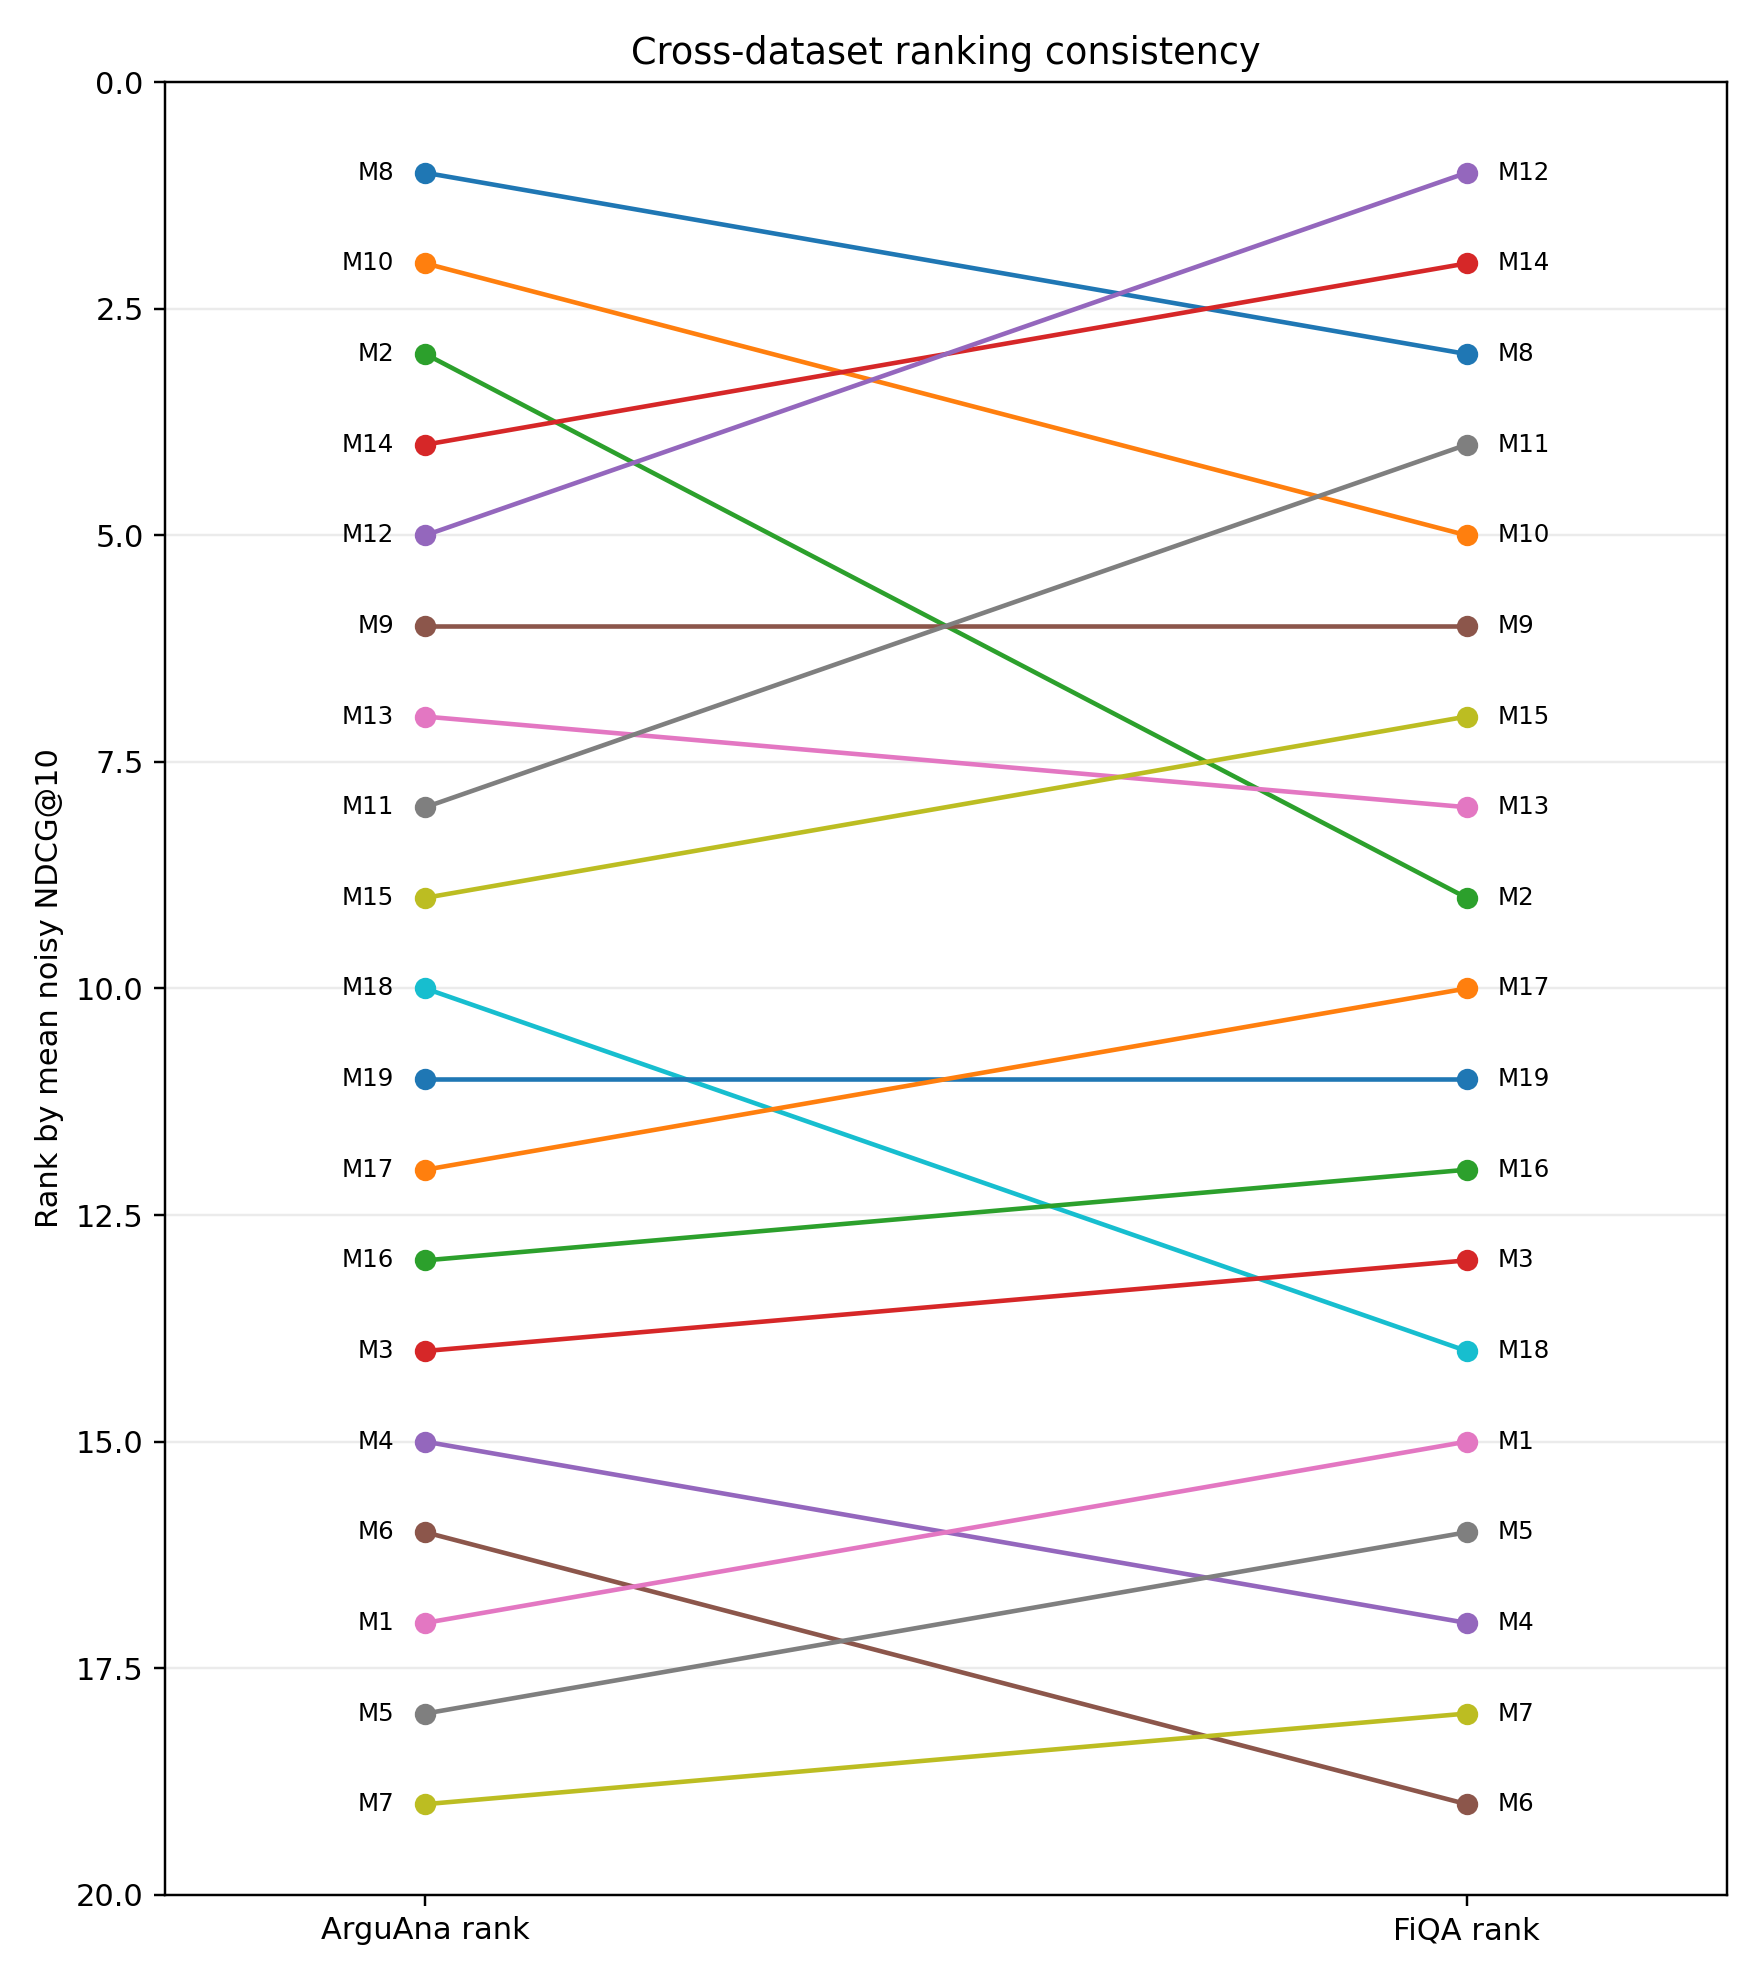
\includegraphics[width=0.68\textwidth]{figures/cross_dataset_ranks.png}\caption{سازگاری رتبه روش‌ها بین دو مجموعه‌داده}\end{figure}
همبستگی رتبه‌ای اسپیرمن رتبه روش‌ها بر اساس میانگین NDCG نویزی برابر $0.882$ بود. روش‌های ۸ تا ۱۵ در هر دو دامنه در نیمه بالای جدول قرار گرفتند.

\begin{figure}[H]\centering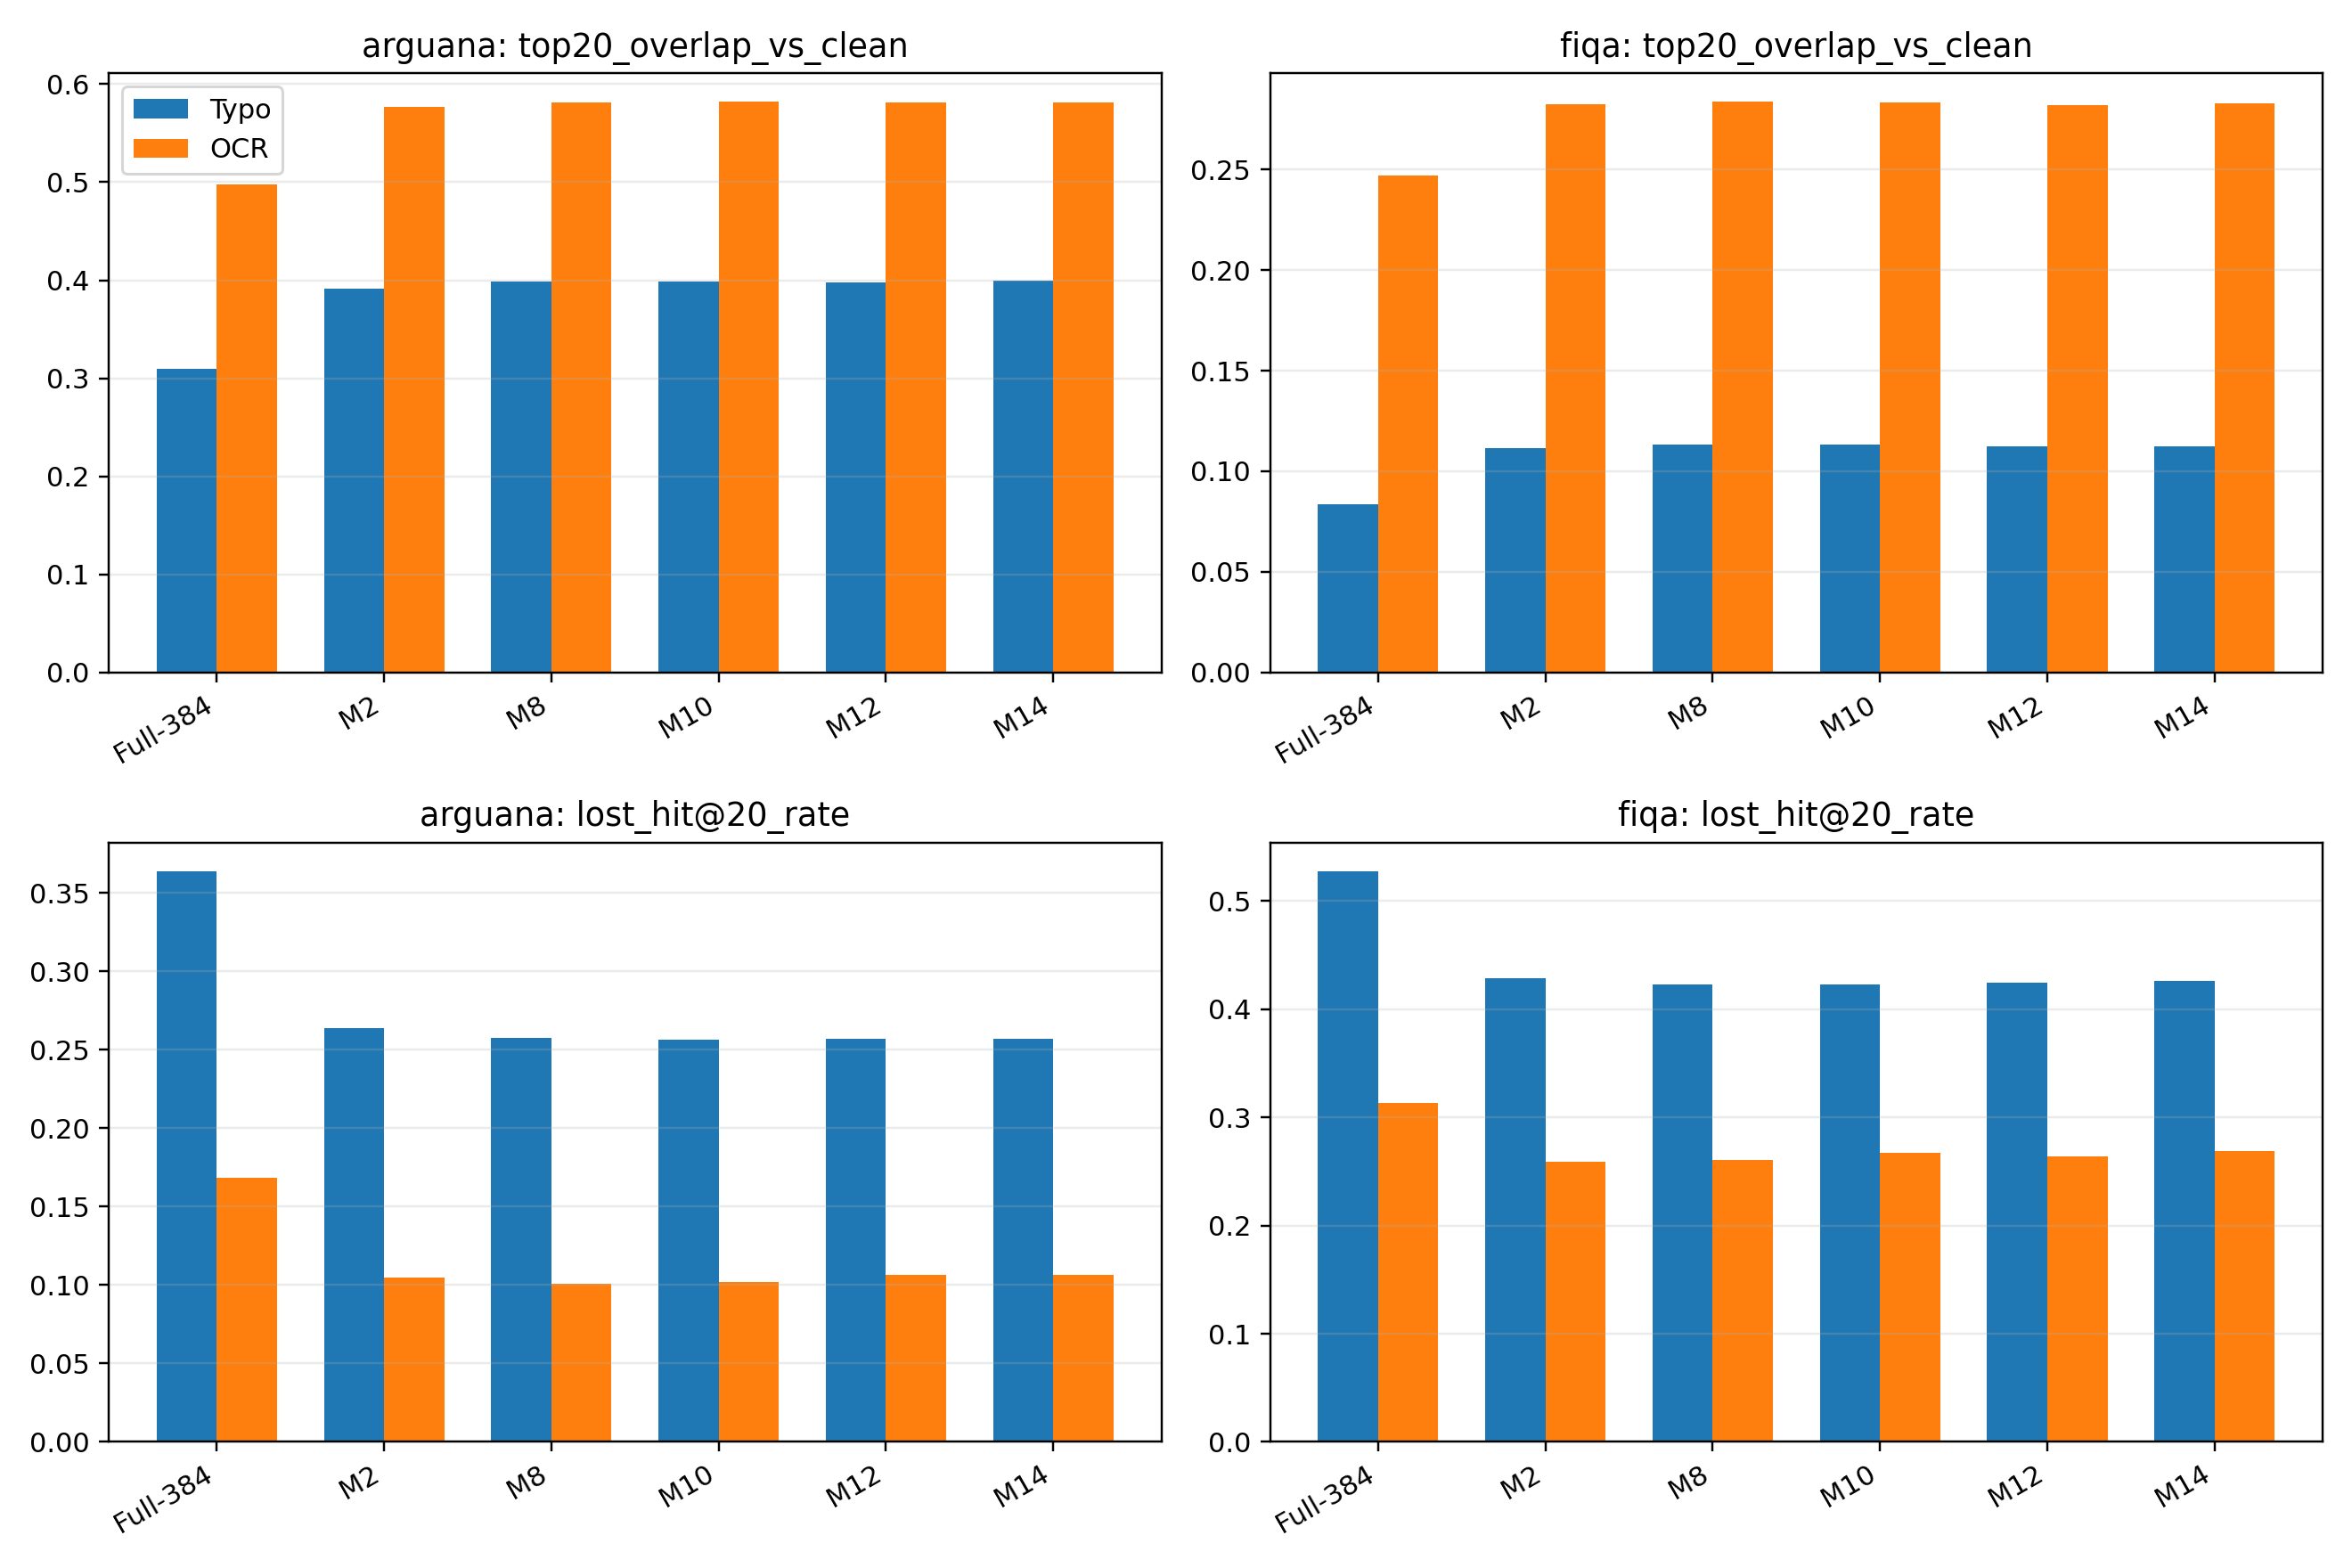
\includegraphics[width=\textwidth]{figures/robustness_selected.png}\caption{هم‌پوشانی ۲۰ نتیجه و نرخ از دست‌رفتن hit برای روش‌های منتخب}\end{figure}

\begin{figure}[H]\centering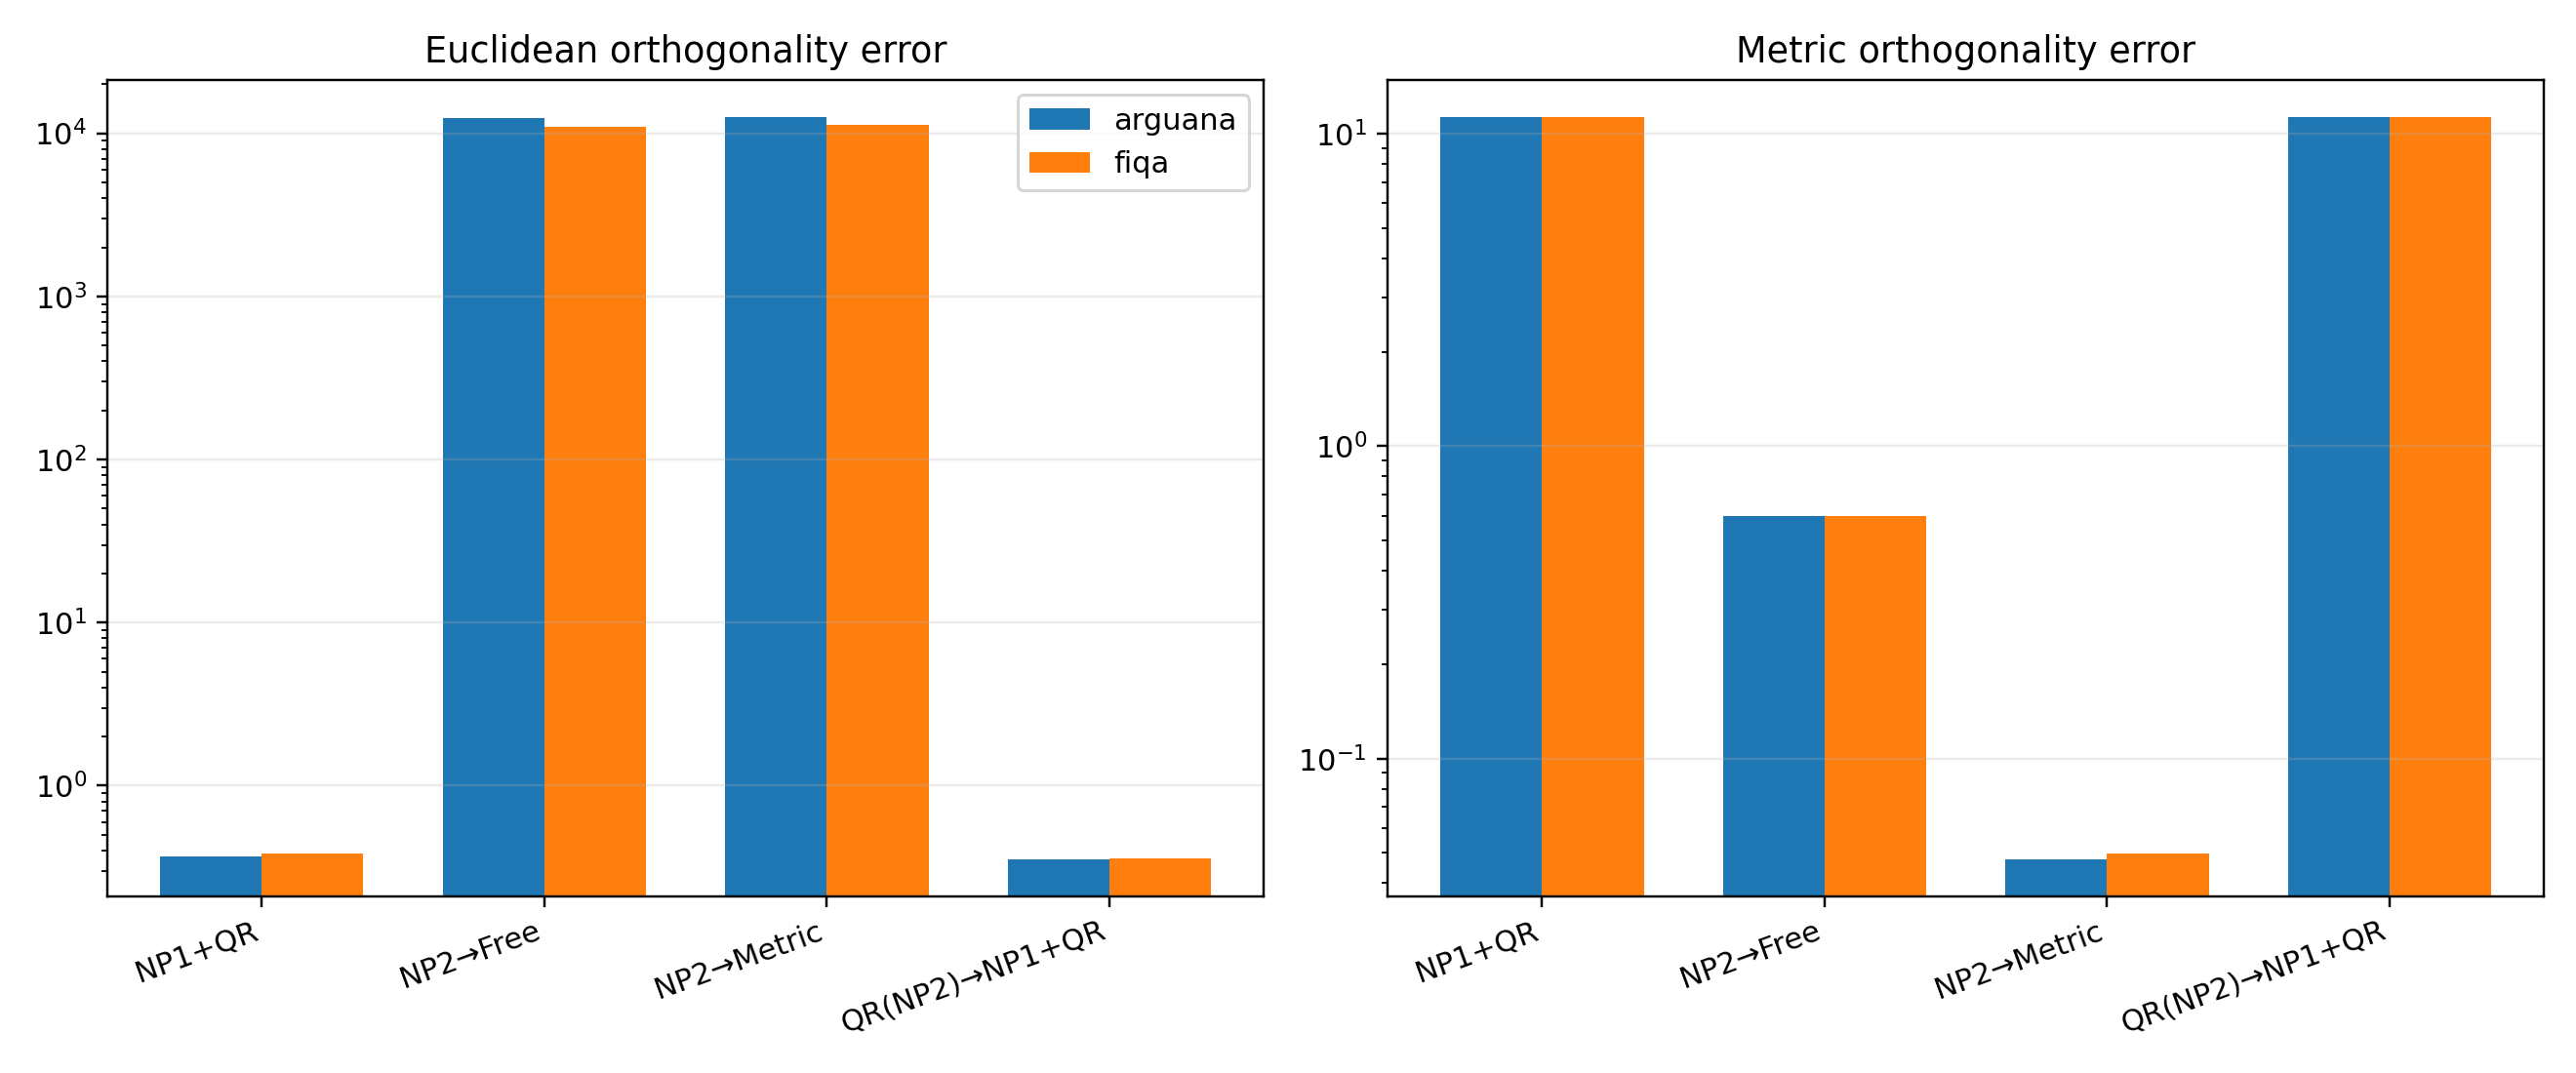
\includegraphics[width=\textwidth]{figures/geometry_family.png}\caption{خطای متعامدسازی اقلیدسی و متریکی خانواده‌ها در مقیاس لگاریتمی}\end{figure}
کمترین خطای هندسی الزاماً بهترین retrieval را تولید نکرد. متعامدسازی یک محدودیت طراحی است و معیار نهایی انتخاب باید کیفیت retrieval باشد.

\subsection{حافظه و زمان}
کاهش بُعد حافظه ماتریس پیکره را دقیقاً به یک‌سوم رساند: در \lr{ArguAna} از $12.706$ به $4.235$ مگابایت و در \lr{FiQA} از $84.431$ به $28.144$ مگابایت.
\scriptsize
\begin{longtable}{|C{3.5cm}|C{1.8cm}|C{2.5cm}|C{3cm}|C{2.5cm}|}
\caption{هزینه روش‌های منتخب روی ArguAna}\label{tab:arg-resource}\\
\hline
\textbf{روش} & \textbf{بُعد} & \textbf{حافظه MB} & \textbf{زمان هر کوئری ms} & \textbf{NDCG تمیز} \\
\hline
\endfirsthead
\hline
\textbf{روش} & \textbf{بُعد} & \textbf{حافظه MB} & \textbf{زمان هر کوئری ms} & \textbf{NDCG تمیز} \\
\hline
\endhead
\lr{Full-384} & 384 & \lr{12.706} & \lr{0.0724} & \lr{0.3711} \\
\hline
\lr{PCA-128} & 128 & \lr{4.235} & \lr{0.0653} & \lr{0.3621} \\
\hline
\lr{SVD-128} & 128 & \lr{4.235} & \lr{0.0525} & \lr{0.3661} \\
\hline
روش 2 & 128 & \lr{4.235} & \lr{0.0505} & \lr{0.3708} \\
\hline
روش 8 & 128 & \lr{4.235} & \lr{0.0541} & \lr{0.3705} \\
\hline
روش 10 & 128 & \lr{4.235} & \lr{0.0661} & \lr{0.3715} \\
\hline
روش 12 & 128 & \lr{4.235} & \lr{0.0549} & \lr{0.3708} \\
\hline
روش 14 & 128 & \lr{4.235} & \lr{0.0567} & \lr{0.3708} \\
\hline
\end{longtable}
\scriptsize
\begin{longtable}{|C{3.5cm}|C{1.8cm}|C{2.5cm}|C{3cm}|C{2.5cm}|}
\caption{هزینه روش‌های منتخب روی FiQA-2018}\label{tab:fiqa-resource}\\
\hline
\textbf{روش} & \textbf{بُعد} & \textbf{حافظه MB} & \textbf{زمان هر کوئری ms} & \textbf{NDCG تمیز} \\
\hline
\endfirsthead
\hline
\textbf{روش} & \textbf{بُعد} & \textbf{حافظه MB} & \textbf{زمان هر کوئری ms} & \textbf{NDCG تمیز} \\
\hline
\endhead
\lr{Full-384} & 384 & \lr{84.431} & \lr{0.4374} & \lr{0.3687} \\
\hline
\lr{PCA-128} & 128 & \lr{28.144} & \lr{1.4469} & \lr{0.3358} \\
\hline
\lr{SVD-128} & 128 & \lr{28.144} & \lr{1.4605} & \lr{0.3375} \\
\hline
روش 2 & 128 & \lr{28.144} & \lr{1.7022} & \lr{0.3256} \\
\hline
روش 8 & 128 & \lr{28.144} & \lr{2.1818} & \lr{0.3250} \\
\hline
روش 10 & 128 & \lr{28.144} & \lr{1.6537} & \lr{0.3243} \\
\hline
روش 12 & 128 & \lr{28.144} & \lr{1.6798} & \lr{0.3235} \\
\hline
روش 14 & 128 & \lr{28.144} & \lr{1.6986} & \lr{0.3231} \\
\hline
\end{longtable}
زمان جست‌وجو در اجرای تک‌مرحله‌ای نوسان داشت و برای ادعای قطعی شتاب مناسب نیست؛ کاهش حافظه مستقیم و قطعی است.

\section{جمع‌بندی نهایی}
\begin{enumerate}
\item روش ۲ یک مرجع بسته و قوی است.
\item خانواده‌های ۸ تا ۱۵ در هر دو دامنه بهترین‌اند.
\item پروژکتور عمومی و مقداردهی روش ۲ از متعامدسازی اقلیدسی مهم‌تر است.
\item ترم حذف نویز در \lr{ArguAna} و خانواده متریکی \lr{FiQA} مؤثر است؛ ترم حفظ سیگنال اغلب قابل حذف است.
\item برتری بر بردار کامل واقعی ولی وابسته به دامنه و شدت نویز است.
\item روش‌های ۲، ۸، ۱۰، ۱۲، ۱۴ و برای بدترین‌حالت روش ۱۵ باید در مرحله چندبذری حفظ شوند.
\end{enumerate}
محدودیت اصلی، یک بذر آموزش و یک بذر نویز است. برای ادعای آماری نهایی، چند بذر و نویزهای دیده‌نشده لازم است.

\appendix
\section{جداول کامل معیارهای برش ۱۰}

\begin{landscape}
\scriptsize
\begin{longtable}{|C{2.5cm}|C{2cm}|C{2cm}|C{2cm}|C{2.2cm}|C{2cm}|C{2cm}|}
\caption{معیارهای کامل تمیز روی ArguAna}\label{tab:arguana-clean-k10}\\
\hline
\textbf{روش} & \textbf{NDCG@10} & \textbf{MRR@10} & \textbf{Recall@10} & \textbf{Precision@10} & \textbf{MAP@10} & \textbf{Hit@10} \\
\hline
\endfirsthead
\hline
\textbf{روش} & \textbf{NDCG@10} & \textbf{MRR@10} & \textbf{Recall@10} & \textbf{Precision@10} & \textbf{MAP@10} & \textbf{Hit@10} \\
\hline
\endhead
\lr{Full-384} & \lr{0.3711} & \lr{0.2454} & \lr{0.7680} & \lr{0.0768} & \lr{0.2454} & \lr{0.7680} \\
\hline
\lr{PCA-128} & \lr{0.3621} & \lr{0.2386} & \lr{0.7530} & \lr{0.0753} & \lr{0.2386} & \lr{0.7530} \\
\hline
\lr{SVD-128} & \lr{0.3661} & \lr{0.2415} & \lr{0.7609} & \lr{0.0761} & \lr{0.2415} & \lr{0.7609} \\
\hline
\lr{Random-128} & \lr{0.3423} & \lr{0.2261} & \lr{0.7095} & \lr{0.0709} & \lr{0.2261} & \lr{0.7095} \\
\hline
روش 1 & \lr{0.3539} & \lr{0.2311} & \lr{0.7445} & \lr{0.0744} & \lr{0.2311} & \lr{0.7445} \\
\hline
روش 2 & \lr{0.3708} & \lr{0.2470} & \lr{0.7609} & \lr{0.0761} & \lr{0.2470} & \lr{0.7609} \\
\hline
روش 3 & \lr{0.3640} & \lr{0.2401} & \lr{0.7566} & \lr{0.0757} & \lr{0.2401} & \lr{0.7566} \\
\hline
روش 4 & \lr{0.3544} & \lr{0.2311} & \lr{0.7473} & \lr{0.0747} & \lr{0.2311} & \lr{0.7473} \\
\hline
روش 5 & \lr{0.3531} & \lr{0.2304} & \lr{0.7438} & \lr{0.0744} & \lr{0.2304} & \lr{0.7438} \\
\hline
روش 6 & \lr{0.3540} & \lr{0.2312} & \lr{0.7452} & \lr{0.0745} & \lr{0.2312} & \lr{0.7452} \\
\hline
روش 7 & \lr{0.3529} & \lr{0.2304} & \lr{0.7430} & \lr{0.0743} & \lr{0.2304} & \lr{0.7430} \\
\hline
روش 8 & \lr{0.3705} & \lr{0.2469} & \lr{0.7602} & \lr{0.0760} & \lr{0.2469} & \lr{0.7602} \\
\hline
روش 9 & \lr{0.3697} & \lr{0.2463} & \lr{0.7587} & \lr{0.0759} & \lr{0.2463} & \lr{0.7587} \\
\hline
روش 10 & \lr{0.3715} & \lr{0.2476} & \lr{0.7623} & \lr{0.0762} & \lr{0.2476} & \lr{0.7623} \\
\hline
روش 11 & \lr{0.3703} & \lr{0.2472} & \lr{0.7580} & \lr{0.0758} & \lr{0.2472} & \lr{0.7580} \\
\hline
روش 12 & \lr{0.3708} & \lr{0.2471} & \lr{0.7609} & \lr{0.0761} & \lr{0.2471} & \lr{0.7609} \\
\hline
روش 13 & \lr{0.3699} & \lr{0.2462} & \lr{0.7602} & \lr{0.0760} & \lr{0.2462} & \lr{0.7602} \\
\hline
روش 14 & \lr{0.3708} & \lr{0.2471} & \lr{0.7609} & \lr{0.0761} & \lr{0.2471} & \lr{0.7609} \\
\hline
روش 15 & \lr{0.3704} & \lr{0.2467} & \lr{0.7602} & \lr{0.0760} & \lr{0.2467} & \lr{0.7602} \\
\hline
روش 16 & \lr{0.3635} & \lr{0.2400} & \lr{0.7545} & \lr{0.0754} & \lr{0.2400} & \lr{0.7545} \\
\hline
روش 17 & \lr{0.3639} & \lr{0.2398} & \lr{0.7566} & \lr{0.0757} & \lr{0.2398} & \lr{0.7566} \\
\hline
روش 18 & \lr{0.3642} & \lr{0.2402} & \lr{0.7566} & \lr{0.0757} & \lr{0.2402} & \lr{0.7566} \\
\hline
روش 19 & \lr{0.3641} & \lr{0.2401} & \lr{0.7566} & \lr{0.0757} & \lr{0.2401} & \lr{0.7566} \\
\hline
\end{longtable}
\end{landscape}

\begin{landscape}
\scriptsize
\begin{longtable}{|C{2.5cm}|C{2cm}|C{2cm}|C{2cm}|C{2.2cm}|C{2cm}|C{2cm}|}
\caption{معیارهای کامل نویز تایپی روی ArguAna}\label{tab:arguana-queries-only--custom--typo-char-0p150-k10}\\
\hline
\textbf{روش} & \textbf{NDCG@10} & \textbf{MRR@10} & \textbf{Recall@10} & \textbf{Precision@10} & \textbf{MAP@10} & \textbf{Hit@10} \\
\hline
\endfirsthead
\hline
\textbf{روش} & \textbf{NDCG@10} & \textbf{MRR@10} & \textbf{Recall@10} & \textbf{Precision@10} & \textbf{MAP@10} & \textbf{Hit@10} \\
\hline
\endhead
\lr{Full-384} & \lr{0.1911} & \lr{0.1206} & \lr{0.4226} & \lr{0.0423} & \lr{0.1206} & \lr{0.4226} \\
\hline
\lr{PCA-128} & \lr{0.1771} & \lr{0.1157} & \lr{0.3783} & \lr{0.0378} & \lr{0.1157} & \lr{0.3783} \\
\hline
\lr{SVD-128} & \lr{0.1850} & \lr{0.1179} & \lr{0.4054} & \lr{0.0405} & \lr{0.1179} & \lr{0.4054} \\
\hline
\lr{Random-128} & \lr{0.1137} & \lr{0.0735} & \lr{0.2463} & \lr{0.0246} & \lr{0.0735} & \lr{0.2463} \\
\hline
روش 1 & \lr{0.1897} & \lr{0.1241} & \lr{0.4033} & \lr{0.0403} & \lr{0.1241} & \lr{0.4033} \\
\hline
روش 2 & \lr{0.2394} & \lr{0.1558} & \lr{0.5111} & \lr{0.0511} & \lr{0.1558} & \lr{0.5111} \\
\hline
روش 3 & \lr{0.2195} & \lr{0.1422} & \lr{0.4711} & \lr{0.0471} & \lr{0.1422} & \lr{0.4711} \\
\hline
روش 4 & \lr{0.1905} & \lr{0.1245} & \lr{0.4047} & \lr{0.0405} & \lr{0.1245} & \lr{0.4047} \\
\hline
روش 5 & \lr{0.1894} & \lr{0.1242} & \lr{0.4011} & \lr{0.0401} & \lr{0.1242} & \lr{0.4011} \\
\hline
روش 6 & \lr{0.1906} & \lr{0.1250} & \lr{0.4040} & \lr{0.0404} & \lr{0.1250} & \lr{0.4040} \\
\hline
روش 7 & \lr{0.1892} & \lr{0.1241} & \lr{0.4004} & \lr{0.0400} & \lr{0.1241} & \lr{0.4004} \\
\hline
روش 8 & \lr{0.2393} & \lr{0.1543} & \lr{0.5146} & \lr{0.0515} & \lr{0.1543} & \lr{0.5146} \\
\hline
روش 9 & \lr{0.2315} & \lr{0.1490} & \lr{0.4996} & \lr{0.0500} & \lr{0.1490} & \lr{0.4996} \\
\hline
روش 10 & \lr{0.2395} & \lr{0.1539} & \lr{0.5175} & \lr{0.0517} & \lr{0.1539} & \lr{0.5175} \\
\hline
روش 11 & \lr{0.2311} & \lr{0.1487} & \lr{0.4989} & \lr{0.0499} & \lr{0.1487} & \lr{0.4989} \\
\hline
روش 12 & \lr{0.2380} & \lr{0.1540} & \lr{0.5103} & \lr{0.0510} & \lr{0.1540} & \lr{0.5103} \\
\hline
روش 13 & \lr{0.2317} & \lr{0.1491} & \lr{0.5004} & \lr{0.0500} & \lr{0.1491} & \lr{0.5004} \\
\hline
روش 14 & \lr{0.2386} & \lr{0.1540} & \lr{0.5132} & \lr{0.0513} & \lr{0.1540} & \lr{0.5132} \\
\hline
روش 15 & \lr{0.2308} & \lr{0.1488} & \lr{0.4975} & \lr{0.0498} & \lr{0.1488} & \lr{0.4975} \\
\hline
روش 16 & \lr{0.2245} & \lr{0.1463} & \lr{0.4782} & \lr{0.0478} & \lr{0.1463} & \lr{0.4782} \\
\hline
روش 17 & \lr{0.2253} & \lr{0.1469} & \lr{0.4797} & \lr{0.0480} & \lr{0.1469} & \lr{0.4797} \\
\hline
روش 18 & \lr{0.2255} & \lr{0.1476} & \lr{0.4782} & \lr{0.0478} & \lr{0.1476} & \lr{0.4782} \\
\hline
روش 19 & \lr{0.2256} & \lr{0.1473} & \lr{0.4797} & \lr{0.0480} & \lr{0.1473} & \lr{0.4797} \\
\hline
\end{longtable}
\end{landscape}

\begin{landscape}
\scriptsize
\begin{longtable}{|C{2.5cm}|C{2cm}|C{2cm}|C{2cm}|C{2.2cm}|C{2cm}|C{2cm}|}
\caption{معیارهای کامل نویز مشابه OCR روی ArguAna}\label{tab:arguana-queries-only--custom--ocr-error-0p150-k10}\\
\hline
\textbf{روش} & \textbf{NDCG@10} & \textbf{MRR@10} & \textbf{Recall@10} & \textbf{Precision@10} & \textbf{MAP@10} & \textbf{Hit@10} \\
\hline
\endfirsthead
\hline
\textbf{روش} & \textbf{NDCG@10} & \textbf{MRR@10} & \textbf{Recall@10} & \textbf{Precision@10} & \textbf{MAP@10} & \textbf{Hit@10} \\
\hline
\endhead
\lr{Full-384} & \lr{0.2865} & \lr{0.1887} & \lr{0.5981} & \lr{0.0598} & \lr{0.1887} & \lr{0.5981} \\
\hline
\lr{PCA-128} & \lr{0.2727} & \lr{0.1787} & \lr{0.5739} & \lr{0.0574} & \lr{0.1787} & \lr{0.5739} \\
\hline
\lr{SVD-128} & \lr{0.2813} & \lr{0.1844} & \lr{0.5924} & \lr{0.0592} & \lr{0.1844} & \lr{0.5924} \\
\hline
\lr{Random-128} & \lr{0.2157} & \lr{0.1401} & \lr{0.4611} & \lr{0.0461} & \lr{0.1401} & \lr{0.4611} \\
\hline
روش 1 & \lr{0.2702} & \lr{0.1769} & \lr{0.5689} & \lr{0.0569} & \lr{0.1769} & \lr{0.5689} \\
\hline
روش 2 & \lr{0.3118} & \lr{0.2058} & \lr{0.6481} & \lr{0.0648} & \lr{0.2058} & \lr{0.6481} \\
\hline
روش 3 & \lr{0.2980} & \lr{0.1952} & \lr{0.6260} & \lr{0.0626} & \lr{0.1952} & \lr{0.6260} \\
\hline
روش 4 & \lr{0.2710} & \lr{0.1770} & \lr{0.5724} & \lr{0.0572} & \lr{0.1770} & \lr{0.5724} \\
\hline
روش 5 & \lr{0.2696} & \lr{0.1765} & \lr{0.5682} & \lr{0.0568} & \lr{0.1765} & \lr{0.5682} \\
\hline
روش 6 & \lr{0.2694} & \lr{0.1766} & \lr{0.5667} & \lr{0.0567} & \lr{0.1766} & \lr{0.5667} \\
\hline
روش 7 & \lr{0.2698} & \lr{0.1767} & \lr{0.5682} & \lr{0.0568} & \lr{0.1767} & \lr{0.5682} \\
\hline
روش 8 & \lr{0.3132} & \lr{0.2050} & \lr{0.6581} & \lr{0.0658} & \lr{0.2050} & \lr{0.6581} \\
\hline
روش 9 & \lr{0.3120} & \lr{0.2040} & \lr{0.6574} & \lr{0.0657} & \lr{0.2040} & \lr{0.6574} \\
\hline
روش 10 & \lr{0.3124} & \lr{0.2044} & \lr{0.6567} & \lr{0.0657} & \lr{0.2044} & \lr{0.6567} \\
\hline
روش 11 & \lr{0.3105} & \lr{0.2028} & \lr{0.6545} & \lr{0.0655} & \lr{0.2028} & \lr{0.6545} \\
\hline
روش 12 & \lr{0.3122} & \lr{0.2046} & \lr{0.6552} & \lr{0.0655} & \lr{0.2046} & \lr{0.6552} \\
\hline
روش 13 & \lr{0.3105} & \lr{0.2037} & \lr{0.6510} & \lr{0.0651} & \lr{0.2037} & \lr{0.6510} \\
\hline
روش 14 & \lr{0.3118} & \lr{0.2044} & \lr{0.6545} & \lr{0.0655} & \lr{0.2044} & \lr{0.6545} \\
\hline
روش 15 & \lr{0.3103} & \lr{0.2034} & \lr{0.6517} & \lr{0.0652} & \lr{0.2034} & \lr{0.6517} \\
\hline
روش 16 & \lr{0.2989} & \lr{0.1965} & \lr{0.6260} & \lr{0.0626} & \lr{0.1965} & \lr{0.6260} \\
\hline
روش 17 & \lr{0.2990} & \lr{0.1963} & \lr{0.6274} & \lr{0.0627} & \lr{0.1963} & \lr{0.6274} \\
\hline
روش 18 & \lr{0.3002} & \lr{0.1970} & \lr{0.6303} & \lr{0.0630} & \lr{0.1970} & \lr{0.6303} \\
\hline
روش 19 & \lr{0.2999} & \lr{0.1968} & \lr{0.6296} & \lr{0.0630} & \lr{0.1968} & \lr{0.6296} \\
\hline
\end{longtable}
\end{landscape}

\begin{landscape}
\scriptsize
\begin{longtable}{|C{2.5cm}|C{2cm}|C{2cm}|C{2cm}|C{2.2cm}|C{2cm}|C{2cm}|}
\caption{معیارهای کامل تمیز روی FiQA-2018}\label{tab:fiqa-clean-k10}\\
\hline
\textbf{روش} & \textbf{NDCG@10} & \textbf{MRR@10} & \textbf{Recall@10} & \textbf{Precision@10} & \textbf{MAP@10} & \textbf{Hit@10} \\
\hline
\endfirsthead
\hline
\textbf{روش} & \textbf{NDCG@10} & \textbf{MRR@10} & \textbf{Recall@10} & \textbf{Precision@10} & \textbf{MAP@10} & \textbf{Hit@10} \\
\hline
\endhead
\lr{Full-384} & \lr{0.3687} & \lr{0.4451} & \lr{0.4413} & \lr{0.1045} & \lr{0.2914} & \lr{0.6574} \\
\hline
\lr{PCA-128} & \lr{0.3358} & \lr{0.4118} & \lr{0.4021} & \lr{0.0958} & \lr{0.2618} & \lr{0.6219} \\
\hline
\lr{SVD-128} & \lr{0.3375} & \lr{0.4173} & \lr{0.3997} & \lr{0.0957} & \lr{0.2647} & \lr{0.6111} \\
\hline
\lr{Random-128} & \lr{0.2941} & \lr{0.3568} & \lr{0.3579} & \lr{0.0823} & \lr{0.2289} & \lr{0.5556} \\
\hline
روش 1 & \lr{0.3049} & \lr{0.3749} & \lr{0.3768} & \lr{0.0894} & \lr{0.2319} & \lr{0.5926} \\
\hline
روش 2 & \lr{0.3256} & \lr{0.4067} & \lr{0.3837} & \lr{0.0909} & \lr{0.2550} & \lr{0.5880} \\
\hline
روش 3 & \lr{0.3373} & \lr{0.4145} & \lr{0.4040} & \lr{0.0966} & \lr{0.2626} & \lr{0.6157} \\
\hline
روش 4 & \lr{0.3044} & \lr{0.3756} & \lr{0.3752} & \lr{0.0892} & \lr{0.2316} & \lr{0.5910} \\
\hline
روش 5 & \lr{0.3044} & \lr{0.3765} & \lr{0.3751} & \lr{0.0892} & \lr{0.2316} & \lr{0.5880} \\
\hline
روش 6 & \lr{0.3045} & \lr{0.3742} & \lr{0.3773} & \lr{0.0895} & \lr{0.2314} & \lr{0.5926} \\
\hline
روش 7 & \lr{0.3042} & \lr{0.3757} & \lr{0.3744} & \lr{0.0890} & \lr{0.2317} & \lr{0.5864} \\
\hline
روش 8 & \lr{0.3250} & \lr{0.4048} & \lr{0.3836} & \lr{0.0909} & \lr{0.2545} & \lr{0.5880} \\
\hline
روش 9 & \lr{0.3256} & \lr{0.4063} & \lr{0.3823} & \lr{0.0909} & \lr{0.2554} & \lr{0.5895} \\
\hline
روش 10 & \lr{0.3243} & \lr{0.4041} & \lr{0.3825} & \lr{0.0909} & \lr{0.2538} & \lr{0.5864} \\
\hline
روش 11 & \lr{0.3244} & \lr{0.4046} & \lr{0.3811} & \lr{0.0904} & \lr{0.2544} & \lr{0.5849} \\
\hline
روش 12 & \lr{0.3235} & \lr{0.4045} & \lr{0.3797} & \lr{0.0904} & \lr{0.2535} & \lr{0.5849} \\
\hline
روش 13 & \lr{0.3231} & \lr{0.4021} & \lr{0.3811} & \lr{0.0903} & \lr{0.2531} & \lr{0.5849} \\
\hline
روش 14 & \lr{0.3231} & \lr{0.4032} & \lr{0.3804} & \lr{0.0906} & \lr{0.2528} & \lr{0.5864} \\
\hline
روش 15 & \lr{0.3235} & \lr{0.4026} & \lr{0.3810} & \lr{0.0903} & \lr{0.2536} & \lr{0.5864} \\
\hline
روش 16 & \lr{0.3220} & \lr{0.3973} & \lr{0.3874} & \lr{0.0927} & \lr{0.2490} & \lr{0.6034} \\
\hline
روش 17 & \lr{0.3234} & \lr{0.3975} & \lr{0.3916} & \lr{0.0934} & \lr{0.2497} & \lr{0.6065} \\
\hline
روش 18 & \lr{0.3214} & \lr{0.3958} & \lr{0.3861} & \lr{0.0921} & \lr{0.2491} & \lr{0.5988} \\
\hline
روش 19 & \lr{0.3219} & \lr{0.3961} & \lr{0.3884} & \lr{0.0929} & \lr{0.2489} & \lr{0.6034} \\
\hline
\end{longtable}
\end{landscape}

\begin{landscape}
\scriptsize
\begin{longtable}{|C{2.5cm}|C{2cm}|C{2cm}|C{2cm}|C{2.2cm}|C{2cm}|C{2cm}|}
\caption{معیارهای کامل نویز تایپی روی FiQA-2018}\label{tab:fiqa-queries-only--custom--typo-char-0p150-k10}\\
\hline
\textbf{روش} & \textbf{NDCG@10} & \textbf{MRR@10} & \textbf{Recall@10} & \textbf{Precision@10} & \textbf{MAP@10} & \textbf{Hit@10} \\
\hline
\endfirsthead
\hline
\textbf{روش} & \textbf{NDCG@10} & \textbf{MRR@10} & \textbf{Recall@10} & \textbf{Precision@10} & \textbf{MAP@10} & \textbf{Hit@10} \\
\hline
\endhead
\lr{Full-384} & \lr{0.0678} & \lr{0.0819} & \lr{0.0954} & \lr{0.0215} & \lr{0.0465} & \lr{0.1682} \\
\hline
\lr{PCA-128} & \lr{0.0448} & \lr{0.0542} & \lr{0.0651} & \lr{0.0150} & \lr{0.0293} & \lr{0.1219} \\
\hline
\lr{SVD-128} & \lr{0.0491} & \lr{0.0595} & \lr{0.0747} & \lr{0.0168} & \lr{0.0312} & \lr{0.1312} \\
\hline
\lr{Random-128} & \lr{0.0381} & \lr{0.0441} & \lr{0.0545} & \lr{0.0120} & \lr{0.0265} & \lr{0.0957} \\
\hline
روش 1 & \lr{0.0476} & \lr{0.0621} & \lr{0.0641} & \lr{0.0162} & \lr{0.0317} & \lr{0.1281} \\
\hline
روش 2 & \lr{0.0774} & \lr{0.0949} & \lr{0.1082} & \lr{0.0239} & \lr{0.0532} & \lr{0.1867} \\
\hline
روش 3 & \lr{0.0649} & \lr{0.0793} & \lr{0.0894} & \lr{0.0202} & \lr{0.0451} & \lr{0.1605} \\
\hline
روش 4 & \lr{0.0472} & \lr{0.0606} & \lr{0.0630} & \lr{0.0159} & \lr{0.0320} & \lr{0.1265} \\
\hline
روش 5 & \lr{0.0465} & \lr{0.0593} & \lr{0.0637} & \lr{0.0160} & \lr{0.0308} & \lr{0.1281} \\
\hline
روش 6 & \lr{0.0453} & \lr{0.0582} & \lr{0.0618} & \lr{0.0154} & \lr{0.0301} & \lr{0.1219} \\
\hline
روش 7 & \lr{0.0456} & \lr{0.0581} & \lr{0.0633} & \lr{0.0156} & \lr{0.0301} & \lr{0.1235} \\
\hline
روش 8 & \lr{0.0787} & \lr{0.0974} & \lr{0.1096} & \lr{0.0245} & \lr{0.0539} & \lr{0.1898} \\
\hline
روش 9 & \lr{0.0792} & \lr{0.0986} & \lr{0.1112} & \lr{0.0245} & \lr{0.0539} & \lr{0.1914} \\
\hline
روش 10 & \lr{0.0793} & \lr{0.0983} & \lr{0.1106} & \lr{0.0245} & \lr{0.0544} & \lr{0.1898} \\
\hline
روش 11 & \lr{0.0802} & \lr{0.1005} & \lr{0.1111} & \lr{0.0245} & \lr{0.0551} & \lr{0.1929} \\
\hline
روش 12 & \lr{0.0796} & \lr{0.0985} & \lr{0.1106} & \lr{0.0247} & \lr{0.0546} & \lr{0.1914} \\
\hline
روش 13 & \lr{0.0807} & \lr{0.1004} & \lr{0.1126} & \lr{0.0248} & \lr{0.0554} & \lr{0.1944} \\
\hline
روش 14 & \lr{0.0800} & \lr{0.0985} & \lr{0.1128} & \lr{0.0247} & \lr{0.0546} & \lr{0.1914} \\
\hline
روش 15 & \lr{0.0812} & \lr{0.1005} & \lr{0.1142} & \lr{0.0250} & \lr{0.0556} & \lr{0.1960} \\
\hline
روش 16 & \lr{0.0608} & \lr{0.0784} & \lr{0.0820} & \lr{0.0193} & \lr{0.0413} & \lr{0.1497} \\
\hline
روش 17 & \lr{0.0611} & \lr{0.0792} & \lr{0.0814} & \lr{0.0193} & \lr{0.0417} & \lr{0.1497} \\
\hline
روش 18 & \lr{0.0612} & \lr{0.0786} & \lr{0.0825} & \lr{0.0194} & \lr{0.0416} & \lr{0.1512} \\
\hline
روش 19 & \lr{0.0613} & \lr{0.0787} & \lr{0.0827} & \lr{0.0196} & \lr{0.0416} & \lr{0.1528} \\
\hline
\end{longtable}
\end{landscape}

\begin{landscape}
\scriptsize
\begin{longtable}{|C{2.5cm}|C{2cm}|C{2cm}|C{2cm}|C{2.2cm}|C{2cm}|C{2cm}|}
\caption{معیارهای کامل نویز مشابه OCR روی FiQA-2018}\label{tab:fiqa-queries-only--custom--ocr-error-0p150-k10}\\
\hline
\textbf{روش} & \textbf{NDCG@10} & \textbf{MRR@10} & \textbf{Recall@10} & \textbf{Precision@10} & \textbf{MAP@10} & \textbf{Hit@10} \\
\hline
\endfirsthead
\hline
\textbf{روش} & \textbf{NDCG@10} & \textbf{MRR@10} & \textbf{Recall@10} & \textbf{Precision@10} & \textbf{MAP@10} & \textbf{Hit@10} \\
\hline
\endhead
\lr{Full-384} & \lr{0.1756} & \lr{0.2121} & \lr{0.2281} & \lr{0.0508} & \lr{0.1307} & \lr{0.3611} \\
\hline
\lr{PCA-128} & \lr{0.1493} & \lr{0.1809} & \lr{0.1995} & \lr{0.0431} & \lr{0.1081} & \lr{0.3256} \\
\hline
\lr{SVD-128} & \lr{0.1519} & \lr{0.1884} & \lr{0.1984} & \lr{0.0434} & \lr{0.1109} & \lr{0.3318} \\
\hline
\lr{Random-128} & \lr{0.1111} & \lr{0.1364} & \lr{0.1481} & \lr{0.0327} & \lr{0.0802} & \lr{0.2500} \\
\hline
روش 1 & \lr{0.1417} & \lr{0.1811} & \lr{0.1861} & \lr{0.0410} & \lr{0.1013} & \lr{0.3194} \\
\hline
روش 2 & \lr{0.1681} & \lr{0.2137} & \lr{0.2127} & \lr{0.0494} & \lr{0.1234} & \lr{0.3627} \\
\hline
روش 3 & \lr{0.1589} & \lr{0.1969} & \lr{0.2083} & \lr{0.0465} & \lr{0.1158} & \lr{0.3410} \\
\hline
روش 4 & \lr{0.1415} & \lr{0.1797} & \lr{0.1873} & \lr{0.0412} & \lr{0.1008} & \lr{0.3225} \\
\hline
روش 5 & \lr{0.1423} & \lr{0.1817} & \lr{0.1860} & \lr{0.0409} & \lr{0.1022} & \lr{0.3210} \\
\hline
روش 6 & \lr{0.1394} & \lr{0.1774} & \lr{0.1841} & \lr{0.0407} & \lr{0.0991} & \lr{0.3210} \\
\hline
روش 7 & \lr{0.1400} & \lr{0.1779} & \lr{0.1854} & \lr{0.0410} & \lr{0.0994} & \lr{0.3210} \\
\hline
روش 8 & \lr{0.1698} & \lr{0.2149} & \lr{0.2181} & \lr{0.0498} & \lr{0.1238} & \lr{0.3673} \\
\hline
روش 9 & \lr{0.1689} & \lr{0.2138} & \lr{0.2159} & \lr{0.0495} & \lr{0.1236} & \lr{0.3580} \\
\hline
روش 10 & \lr{0.1689} & \lr{0.2135} & \lr{0.2161} & \lr{0.0502} & \lr{0.1232} & \lr{0.3642} \\
\hline
روش 11 & \lr{0.1682} & \lr{0.2127} & \lr{0.2153} & \lr{0.0494} & \lr{0.1229} & \lr{0.3611} \\
\hline
روش 12 & \lr{0.1698} & \lr{0.2140} & \lr{0.2179} & \lr{0.0502} & \lr{0.1242} & \lr{0.3657} \\
\hline
روش 13 & \lr{0.1664} & \lr{0.2105} & \lr{0.2113} & \lr{0.0488} & \lr{0.1221} & \lr{0.3534} \\
\hline
روش 14 & \lr{0.1687} & \lr{0.2126} & \lr{0.2164} & \lr{0.0500} & \lr{0.1232} & \lr{0.3642} \\
\hline
روش 15 & \lr{0.1668} & \lr{0.2103} & \lr{0.2132} & \lr{0.0492} & \lr{0.1219} & \lr{0.3565} \\
\hline
روش 16 & \lr{0.1635} & \lr{0.2094} & \lr{0.2060} & \lr{0.0472} & \lr{0.1193} & \lr{0.3596} \\
\hline
روش 17 & \lr{0.1640} & \lr{0.2097} & \lr{0.2069} & \lr{0.0469} & \lr{0.1201} & \lr{0.3580} \\
\hline
روش 18 & \lr{0.1616} & \lr{0.2068} & \lr{0.2041} & \lr{0.0468} & \lr{0.1176} & \lr{0.3565} \\
\hline
روش 19 & \lr{0.1631} & \lr{0.2097} & \lr{0.2053} & \lr{0.0468} & \lr{0.1191} & \lr{0.3596} \\
\hline
\end{longtable}
\end{landscape}

\section{جداول کامل تغییر معیارها در برش‌های مختلف}

\begin{landscape}
\scriptsize
\begin{longtable}{|C{2.2cm}|C{1.7cm}|C{1.7cm}|C{1.8cm}|C{1.8cm}|C{1.7cm}|C{1.7cm}|C{1.8cm}|C{1.8cm}|}
\caption{تغییر NDCG و Recall در برش‌های مختلف - تمیز - ArguAna}\label{tab:arguana-clean-cutoffs}\\
\hline
\textbf{روش} & \textbf{NDCG@1} & \textbf{NDCG@5} & \textbf{NDCG@10} & \textbf{NDCG@20} & \textbf{Recall@1} & \textbf{Recall@5} & \textbf{Recall@10} & \textbf{Recall@20} \\
\hline
\endfirsthead
\hline
\textbf{روش} & \textbf{NDCG@1} & \textbf{NDCG@5} & \textbf{NDCG@10} & \textbf{NDCG@20} & \textbf{Recall@1} & \textbf{Recall@5} & \textbf{Recall@10} & \textbf{Recall@20} \\
\hline
\endhead
\lr{Full-384} & \lr{0.0000} & \lr{0.3089} & \lr{0.3711} & \lr{0.4067} & \lr{0.0000} & \lr{0.5774} & \lr{0.7680} & \lr{0.9065} \\
\hline
\lr{PCA-128} & \lr{0.0007} & \lr{0.2996} & \lr{0.3621} & \lr{0.3989} & \lr{0.0007} & \lr{0.5610} & \lr{0.7530} & \lr{0.8972} \\
\hline
\lr{SVD-128} & \lr{0.0007} & \lr{0.3032} & \lr{0.3661} & \lr{0.4019} & \lr{0.0007} & \lr{0.5667} & \lr{0.7609} & \lr{0.9015} \\
\hline
\lr{Random-128} & \lr{0.0014} & \lr{0.2824} & \lr{0.3423} & \lr{0.3798} & \lr{0.0014} & \lr{0.5268} & \lr{0.7095} & \lr{0.8565} \\
\hline
روش 1 & \lr{0.0007} & \lr{0.2854} & \lr{0.3539} & \lr{0.3893} & \lr{0.0007} & \lr{0.5339} & \lr{0.7445} & \lr{0.8837} \\
\hline
روش 2 & \lr{0.0007} & \lr{0.3105} & \lr{0.3708} & \lr{0.4051} & \lr{0.0007} & \lr{0.5760} & \lr{0.7609} & \lr{0.8936} \\
\hline
روش 3 & \lr{0.0007} & \lr{0.3029} & \lr{0.3640} & \lr{0.4011} & \lr{0.0007} & \lr{0.5675} & \lr{0.7566} & \lr{0.9022} \\
\hline
روش 4 & \lr{0.0007} & \lr{0.2836} & \lr{0.3544} & \lr{0.3894} & \lr{0.0007} & \lr{0.5289} & \lr{0.7473} & \lr{0.8851} \\
\hline
روش 5 & \lr{0.0007} & \lr{0.2837} & \lr{0.3531} & \lr{0.3890} & \lr{0.0007} & \lr{0.5303} & \lr{0.7438} & \lr{0.8851} \\
\hline
روش 6 & \lr{0.0007} & \lr{0.2848} & \lr{0.3540} & \lr{0.3892} & \lr{0.0007} & \lr{0.5318} & \lr{0.7452} & \lr{0.8837} \\
\hline
روش 7 & \lr{0.0007} & \lr{0.2836} & \lr{0.3529} & \lr{0.3885} & \lr{0.0007} & \lr{0.5296} & \lr{0.7430} & \lr{0.8829} \\
\hline
روش 8 & \lr{0.0007} & \lr{0.3113} & \lr{0.3705} & \lr{0.4045} & \lr{0.0007} & \lr{0.5782} & \lr{0.7602} & \lr{0.8922} \\
\hline
روش 9 & \lr{0.0007} & \lr{0.3095} & \lr{0.3697} & \lr{0.4039} & \lr{0.0007} & \lr{0.5739} & \lr{0.7587} & \lr{0.8915} \\
\hline
روش 10 & \lr{0.0007} & \lr{0.3117} & \lr{0.3715} & \lr{0.4053} & \lr{0.0007} & \lr{0.5782} & \lr{0.7623} & \lr{0.8936} \\
\hline
روش 11 & \lr{0.0007} & \lr{0.3111} & \lr{0.3703} & \lr{0.4045} & \lr{0.0007} & \lr{0.5760} & \lr{0.7580} & \lr{0.8908} \\
\hline
روش 12 & \lr{0.0007} & \lr{0.3111} & \lr{0.3708} & \lr{0.4048} & \lr{0.0007} & \lr{0.5774} & \lr{0.7609} & \lr{0.8929} \\
\hline
روش 13 & \lr{0.0007} & \lr{0.3093} & \lr{0.3699} & \lr{0.4035} & \lr{0.0007} & \lr{0.5739} & \lr{0.7602} & \lr{0.8908} \\
\hline
روش 14 & \lr{0.0007} & \lr{0.3106} & \lr{0.3708} & \lr{0.4048} & \lr{0.0007} & \lr{0.5760} & \lr{0.7609} & \lr{0.8929} \\
\hline
روش 15 & \lr{0.0007} & \lr{0.3094} & \lr{0.3704} & \lr{0.4041} & \lr{0.0007} & \lr{0.5732} & \lr{0.7602} & \lr{0.8915} \\
\hline
روش 16 & \lr{0.0007} & \lr{0.3014} & \lr{0.3635} & \lr{0.3994} & \lr{0.0007} & \lr{0.5632} & \lr{0.7545} & \lr{0.8944} \\
\hline
روش 17 & \lr{0.0000} & \lr{0.3024} & \lr{0.3639} & \lr{0.3989} & \lr{0.0000} & \lr{0.5667} & \lr{0.7566} & \lr{0.8929} \\
\hline
روش 18 & \lr{0.0007} & \lr{0.3009} & \lr{0.3642} & \lr{0.3997} & \lr{0.0007} & \lr{0.5617} & \lr{0.7566} & \lr{0.8951} \\
\hline
روش 19 & \lr{0.0007} & \lr{0.3013} & \lr{0.3641} & \lr{0.3994} & \lr{0.0007} & \lr{0.5632} & \lr{0.7566} & \lr{0.8944} \\
\hline
\end{longtable}
\end{landscape}

\begin{landscape}
\scriptsize
\begin{longtable}{|C{2.2cm}|C{1.7cm}|C{1.7cm}|C{1.8cm}|C{1.8cm}|C{1.7cm}|C{1.7cm}|C{1.8cm}|C{1.8cm}|}
\caption{تغییر NDCG و Recall در برش‌های مختلف - نویز تایپی - ArguAna}\label{tab:arguana-queries-only--custom--typo-char-0p150-cutoffs}\\
\hline
\textbf{روش} & \textbf{NDCG@1} & \textbf{NDCG@5} & \textbf{NDCG@10} & \textbf{NDCG@20} & \textbf{Recall@1} & \textbf{Recall@5} & \textbf{Recall@10} & \textbf{Recall@20} \\
\hline
\endfirsthead
\hline
\textbf{روش} & \textbf{NDCG@1} & \textbf{NDCG@5} & \textbf{NDCG@10} & \textbf{NDCG@20} & \textbf{Recall@1} & \textbf{Recall@5} & \textbf{Recall@10} & \textbf{Recall@20} \\
\hline
\endhead
\lr{Full-384} & \lr{0.0143} & \lr{0.1350} & \lr{0.1911} & \lr{0.2257} & \lr{0.0143} & \lr{0.2491} & \lr{0.4226} & \lr{0.5603} \\
\hline
\lr{PCA-128} & \lr{0.0228} & \lr{0.1275} & \lr{0.1771} & \lr{0.2162} & \lr{0.0228} & \lr{0.2263} & \lr{0.3783} & \lr{0.5318} \\
\hline
\lr{SVD-128} & \lr{0.0157} & \lr{0.1309} & \lr{0.1850} & \lr{0.2202} & \lr{0.0157} & \lr{0.2377} & \lr{0.4054} & \lr{0.5439} \\
\hline
\lr{Random-128} & \lr{0.0143} & \lr{0.0812} & \lr{0.1137} & \lr{0.1377} & \lr{0.0143} & \lr{0.1449} & \lr{0.2463} & \lr{0.3419} \\
\hline
روش 1 & \lr{0.0186} & \lr{0.1450} & \lr{0.1897} & \lr{0.2258} & \lr{0.0186} & \lr{0.2641} & \lr{0.4033} & \lr{0.5439} \\
\hline
روش 2 & \lr{0.0178} & \lr{0.1824} & \lr{0.2394} & \lr{0.2762} & \lr{0.0178} & \lr{0.3333} & \lr{0.5111} & \lr{0.6552} \\
\hline
روش 3 & \lr{0.0193} & \lr{0.1671} & \lr{0.2195} & \lr{0.2571} & \lr{0.0193} & \lr{0.3076} & \lr{0.4711} & \lr{0.6196} \\
\hline
روش 4 & \lr{0.0186} & \lr{0.1443} & \lr{0.1905} & \lr{0.2263} & \lr{0.0186} & \lr{0.2627} & \lr{0.4047} & \lr{0.5446} \\
\hline
روش 5 & \lr{0.0186} & \lr{0.1448} & \lr{0.1894} & \lr{0.2268} & \lr{0.0186} & \lr{0.2634} & \lr{0.4011} & \lr{0.5475} \\
\hline
روش 6 & \lr{0.0193} & \lr{0.1453} & \lr{0.1906} & \lr{0.2269} & \lr{0.0193} & \lr{0.2641} & \lr{0.4040} & \lr{0.5460} \\
\hline
روش 7 & \lr{0.0186} & \lr{0.1450} & \lr{0.1892} & \lr{0.2265} & \lr{0.0186} & \lr{0.2641} & \lr{0.4004} & \lr{0.5460} \\
\hline
روش 8 & \lr{0.0150} & \lr{0.1801} & \lr{0.2393} & \lr{0.2765} & \lr{0.0150} & \lr{0.3319} & \lr{0.5146} & \lr{0.6624} \\
\hline
روش 9 & \lr{0.0143} & \lr{0.1726} & \lr{0.2315} & \lr{0.2703} & \lr{0.0143} & \lr{0.3169} & \lr{0.4996} & \lr{0.6524} \\
\hline
روش 10 & \lr{0.0157} & \lr{0.1788} & \lr{0.2395} & \lr{0.2762} & \lr{0.0157} & \lr{0.3298} & \lr{0.5175} & \lr{0.6638} \\
\hline
روش 11 & \lr{0.0136} & \lr{0.1729} & \lr{0.2311} & \lr{0.2689} & \lr{0.0136} & \lr{0.3183} & \lr{0.4989} & \lr{0.6481} \\
\hline
روش 12 & \lr{0.0157} & \lr{0.1796} & \lr{0.2380} & \lr{0.2764} & \lr{0.0157} & \lr{0.3305} & \lr{0.5103} & \lr{0.6631} \\
\hline
روش 13 & \lr{0.0143} & \lr{0.1728} & \lr{0.2317} & \lr{0.2697} & \lr{0.0143} & \lr{0.3176} & \lr{0.5004} & \lr{0.6502} \\
\hline
روش 14 & \lr{0.0171} & \lr{0.1787} & \lr{0.2386} & \lr{0.2764} & \lr{0.0171} & \lr{0.3283} & \lr{0.5132} & \lr{0.6638} \\
\hline
روش 15 & \lr{0.0150} & \lr{0.1731} & \lr{0.2308} & \lr{0.2692} & \lr{0.0150} & \lr{0.3183} & \lr{0.4975} & \lr{0.6488} \\
\hline
روش 16 & \lr{0.0193} & \lr{0.1724} & \lr{0.2245} & \lr{0.2630} & \lr{0.0193} & \lr{0.3169} & \lr{0.4782} & \lr{0.6303} \\
\hline
روش 17 & \lr{0.0200} & \lr{0.1726} & \lr{0.2253} & \lr{0.2634} & \lr{0.0200} & \lr{0.3162} & \lr{0.4797} & \lr{0.6303} \\
\hline
روش 18 & \lr{0.0207} & \lr{0.1730} & \lr{0.2255} & \lr{0.2642} & \lr{0.0207} & \lr{0.3155} & \lr{0.4782} & \lr{0.6310} \\
\hline
روش 19 & \lr{0.0200} & \lr{0.1729} & \lr{0.2256} & \lr{0.2640} & \lr{0.0200} & \lr{0.3162} & \lr{0.4797} & \lr{0.6317} \\
\hline
\end{longtable}
\end{landscape}

\begin{landscape}
\scriptsize
\begin{longtable}{|C{2.2cm}|C{1.7cm}|C{1.7cm}|C{1.8cm}|C{1.8cm}|C{1.7cm}|C{1.7cm}|C{1.8cm}|C{1.8cm}|}
\caption{تغییر NDCG و Recall در برش‌های مختلف - نویز مشابه OCR - ArguAna}\label{tab:arguana-queries-only--custom--ocr-error-0p150-cutoffs}\\
\hline
\textbf{روش} & \textbf{NDCG@1} & \textbf{NDCG@5} & \textbf{NDCG@10} & \textbf{NDCG@20} & \textbf{Recall@1} & \textbf{Recall@5} & \textbf{Recall@10} & \textbf{Recall@20} \\
\hline
\endfirsthead
\hline
\textbf{روش} & \textbf{NDCG@1} & \textbf{NDCG@5} & \textbf{NDCG@10} & \textbf{NDCG@20} & \textbf{Recall@1} & \textbf{Recall@5} & \textbf{Recall@10} & \textbf{Recall@20} \\
\hline
\endhead
\lr{Full-384} & \lr{0.0086} & \lr{0.2312} & \lr{0.2865} & \lr{0.3265} & \lr{0.0086} & \lr{0.4290} & \lr{0.5981} & \lr{0.7559} \\
\hline
\lr{PCA-128} & \lr{0.0086} & \lr{0.2143} & \lr{0.2727} & \lr{0.3103} & \lr{0.0086} & \lr{0.3947} & \lr{0.5739} & \lr{0.7223} \\
\hline
\lr{SVD-128} & \lr{0.0100} & \lr{0.2208} & \lr{0.2813} & \lr{0.3174} & \lr{0.0100} & \lr{0.4061} & \lr{0.5924} & \lr{0.7352} \\
\hline
\lr{Random-128} & \lr{0.0171} & \lr{0.1630} & \lr{0.2157} & \lr{0.2504} & \lr{0.0171} & \lr{0.2984} & \lr{0.4611} & \lr{0.5974} \\
\hline
روش 1 & \lr{0.0128} & \lr{0.2170} & \lr{0.2702} & \lr{0.3132} & \lr{0.0128} & \lr{0.4054} & \lr{0.5689} & \lr{0.7366} \\
\hline
روش 2 & \lr{0.0057} & \lr{0.2574} & \lr{0.3118} & \lr{0.3545} & \lr{0.0057} & \lr{0.4818} & \lr{0.6481} & \lr{0.8144} \\
\hline
روش 3 & \lr{0.0071} & \lr{0.2396} & \lr{0.2980} & \lr{0.3357} & \lr{0.0071} & \lr{0.4461} & \lr{0.6260} & \lr{0.7737} \\
\hline
روش 4 & \lr{0.0128} & \lr{0.2165} & \lr{0.2710} & \lr{0.3141} & \lr{0.0128} & \lr{0.4040} & \lr{0.5724} & \lr{0.7423} \\
\hline
روش 5 & \lr{0.0128} & \lr{0.2161} & \lr{0.2696} & \lr{0.3131} & \lr{0.0128} & \lr{0.4033} & \lr{0.5682} & \lr{0.7388} \\
\hline
روش 6 & \lr{0.0136} & \lr{0.2167} & \lr{0.2694} & \lr{0.3138} & \lr{0.0136} & \lr{0.4040} & \lr{0.5667} & \lr{0.7409} \\
\hline
روش 7 & \lr{0.0128} & \lr{0.2166} & \lr{0.2698} & \lr{0.3131} & \lr{0.0128} & \lr{0.4040} & \lr{0.5682} & \lr{0.7380} \\
\hline
روش 8 & \lr{0.0071} & \lr{0.2539} & \lr{0.3132} & \lr{0.3530} & \lr{0.0071} & \lr{0.4761} & \lr{0.6581} & \lr{0.8144} \\
\hline
روش 9 & \lr{0.0079} & \lr{0.2506} & \lr{0.3120} & \lr{0.3504} & \lr{0.0079} & \lr{0.4682} & \lr{0.6574} & \lr{0.8080} \\
\hline
روش 10 & \lr{0.0071} & \lr{0.2532} & \lr{0.3124} & \lr{0.3526} & \lr{0.0071} & \lr{0.4747} & \lr{0.6567} & \lr{0.8144} \\
\hline
روش 11 & \lr{0.0071} & \lr{0.2494} & \lr{0.3105} & \lr{0.3496} & \lr{0.0071} & \lr{0.4668} & \lr{0.6545} & \lr{0.8080} \\
\hline
روش 12 & \lr{0.0079} & \lr{0.2529} & \lr{0.3122} & \lr{0.3520} & \lr{0.0079} & \lr{0.4732} & \lr{0.6552} & \lr{0.8108} \\
\hline
روش 13 & \lr{0.0086} & \lr{0.2503} & \lr{0.3105} & \lr{0.3503} & \lr{0.0086} & \lr{0.4668} & \lr{0.6510} & \lr{0.8073} \\
\hline
روش 14 & \lr{0.0071} & \lr{0.2527} & \lr{0.3118} & \lr{0.3518} & \lr{0.0071} & \lr{0.4725} & \lr{0.6545} & \lr{0.8108} \\
\hline
روش 15 & \lr{0.0086} & \lr{0.2503} & \lr{0.3103} & \lr{0.3496} & \lr{0.0086} & \lr{0.4675} & \lr{0.6517} & \lr{0.8059} \\
\hline
روش 16 & \lr{0.0093} & \lr{0.2417} & \lr{0.2989} & \lr{0.3412} & \lr{0.0093} & \lr{0.4483} & \lr{0.6260} & \lr{0.7923} \\
\hline
روش 17 & \lr{0.0093} & \lr{0.2416} & \lr{0.2990} & \lr{0.3408} & \lr{0.0093} & \lr{0.4490} & \lr{0.6274} & \lr{0.7916} \\
\hline
روش 18 & \lr{0.0100} & \lr{0.2417} & \lr{0.3002} & \lr{0.3414} & \lr{0.0100} & \lr{0.4483} & \lr{0.6303} & \lr{0.7923} \\
\hline
روش 19 & \lr{0.0100} & \lr{0.2421} & \lr{0.2999} & \lr{0.3410} & \lr{0.0100} & \lr{0.4497} & \lr{0.6296} & \lr{0.7909} \\
\hline
\end{longtable}
\end{landscape}

\begin{landscape}
\scriptsize
\begin{longtable}{|C{2.2cm}|C{1.7cm}|C{1.7cm}|C{1.8cm}|C{1.8cm}|C{1.7cm}|C{1.7cm}|C{1.8cm}|C{1.8cm}|}
\caption{تغییر NDCG و Recall در برش‌های مختلف - تمیز - FiQA-2018}\label{tab:fiqa-clean-cutoffs}\\
\hline
\textbf{روش} & \textbf{NDCG@1} & \textbf{NDCG@5} & \textbf{NDCG@10} & \textbf{NDCG@20} & \textbf{Recall@1} & \textbf{Recall@5} & \textbf{Recall@10} & \textbf{Recall@20} \\
\hline
\endfirsthead
\hline
\textbf{روش} & \textbf{NDCG@1} & \textbf{NDCG@5} & \textbf{NDCG@10} & \textbf{NDCG@20} & \textbf{Recall@1} & \textbf{Recall@5} & \textbf{Recall@10} & \textbf{Recall@20} \\
\hline
\endhead
\lr{Full-384} & \lr{0.3472} & \lr{0.3450} & \lr{0.3687} & \lr{0.3943} & \lr{0.1714} & \lr{0.3671} & \lr{0.4413} & \lr{0.5199} \\
\hline
\lr{PCA-128} & \lr{0.3133} & \lr{0.3127} & \lr{0.3358} & \lr{0.3657} & \lr{0.1564} & \lr{0.3317} & \lr{0.4021} & \lr{0.4979} \\
\hline
\lr{SVD-128} & \lr{0.3302} & \lr{0.3155} & \lr{0.3375} & \lr{0.3658} & \lr{0.1626} & \lr{0.3339} & \lr{0.3997} & \lr{0.4890} \\
\hline
\lr{Random-128} & \lr{0.2716} & \lr{0.2727} & \lr{0.2941} & \lr{0.3147} & \lr{0.1368} & \lr{0.2926} & \lr{0.3579} & \lr{0.4204} \\
\hline
روش 1 & \lr{0.2840} & \lr{0.2821} & \lr{0.3049} & \lr{0.3325} & \lr{0.1380} & \lr{0.3073} & \lr{0.3768} & \lr{0.4632} \\
\hline
روش 2 & \lr{0.3210} & \lr{0.3040} & \lr{0.3256} & \lr{0.3509} & \lr{0.1561} & \lr{0.3161} & \lr{0.3837} & \lr{0.4619} \\
\hline
روش 3 & \lr{0.3194} & \lr{0.3171} & \lr{0.3373} & \lr{0.3651} & \lr{0.1571} & \lr{0.3424} & \lr{0.4040} & \lr{0.4911} \\
\hline
روش 4 & \lr{0.2824} & \lr{0.2800} & \lr{0.3044} & \lr{0.3315} & \lr{0.1366} & \lr{0.3011} & \lr{0.3752} & \lr{0.4601} \\
\hline
روش 5 & \lr{0.2855} & \lr{0.2789} & \lr{0.3044} & \lr{0.3315} & \lr{0.1370} & \lr{0.2986} & \lr{0.3751} & \lr{0.4607} \\
\hline
روش 6 & \lr{0.2824} & \lr{0.2787} & \lr{0.3045} & \lr{0.3319} & \lr{0.1378} & \lr{0.2990} & \lr{0.3773} & \lr{0.4630} \\
\hline
روش 7 & \lr{0.2855} & \lr{0.2783} & \lr{0.3042} & \lr{0.3316} & \lr{0.1383} & \lr{0.2966} & \lr{0.3744} & \lr{0.4603} \\
\hline
روش 8 & \lr{0.3164} & \lr{0.3028} & \lr{0.3250} & \lr{0.3507} & \lr{0.1541} & \lr{0.3137} & \lr{0.3836} & \lr{0.4630} \\
\hline
روش 9 & \lr{0.3179} & \lr{0.3048} & \lr{0.3256} & \lr{0.3520} & \lr{0.1560} & \lr{0.3170} & \lr{0.3823} & \lr{0.4646} \\
\hline
روش 10 & \lr{0.3164} & \lr{0.3021} & \lr{0.3243} & \lr{0.3505} & \lr{0.1536} & \lr{0.3131} & \lr{0.3825} & \lr{0.4644} \\
\hline
روش 11 & \lr{0.3164} & \lr{0.3041} & \lr{0.3244} & \lr{0.3510} & \lr{0.1545} & \lr{0.3170} & \lr{0.3811} & \lr{0.4639} \\
\hline
روش 12 & \lr{0.3179} & \lr{0.3023} & \lr{0.3235} & \lr{0.3500} & \lr{0.1538} & \lr{0.3137} & \lr{0.3797} & \lr{0.4617} \\
\hline
روش 13 & \lr{0.3133} & \lr{0.3013} & \lr{0.3231} & \lr{0.3499} & \lr{0.1524} & \lr{0.3128} & \lr{0.3811} & \lr{0.4643} \\
\hline
روش 14 & \lr{0.3148} & \lr{0.3016} & \lr{0.3231} & \lr{0.3492} & \lr{0.1523} & \lr{0.3137} & \lr{0.3804} & \lr{0.4615} \\
\hline
روش 15 & \lr{0.3133} & \lr{0.3020} & \lr{0.3235} & \lr{0.3500} & \lr{0.1532} & \lr{0.3137} & \lr{0.3810} & \lr{0.4633} \\
\hline
روش 16 & \lr{0.3040} & \lr{0.2976} & \lr{0.3220} & \lr{0.3484} & \lr{0.1501} & \lr{0.3142} & \lr{0.3874} & \lr{0.4693} \\
\hline
روش 17 & \lr{0.3040} & \lr{0.2983} & \lr{0.3234} & \lr{0.3487} & \lr{0.1501} & \lr{0.3151} & \lr{0.3916} & \lr{0.4694} \\
\hline
روش 18 & \lr{0.3025} & \lr{0.2968} & \lr{0.3214} & \lr{0.3466} & \lr{0.1493} & \lr{0.3124} & \lr{0.3861} & \lr{0.4629} \\
\hline
روش 19 & \lr{0.3025} & \lr{0.2976} & \lr{0.3219} & \lr{0.3470} & \lr{0.1491} & \lr{0.3150} & \lr{0.3884} & \lr{0.4658} \\
\hline
\end{longtable}
\end{landscape}

\begin{landscape}
\scriptsize
\begin{longtable}{|C{2.2cm}|C{1.7cm}|C{1.7cm}|C{1.8cm}|C{1.8cm}|C{1.7cm}|C{1.7cm}|C{1.8cm}|C{1.8cm}|}
\caption{تغییر NDCG و Recall در برش‌های مختلف - نویز تایپی - FiQA-2018}\label{tab:fiqa-queries-only--custom--typo-char-0p150-cutoffs}\\
\hline
\textbf{روش} & \textbf{NDCG@1} & \textbf{NDCG@5} & \textbf{NDCG@10} & \textbf{NDCG@20} & \textbf{Recall@1} & \textbf{Recall@5} & \textbf{Recall@10} & \textbf{Recall@20} \\
\hline
\endfirsthead
\hline
\textbf{روش} & \textbf{NDCG@1} & \textbf{NDCG@5} & \textbf{NDCG@10} & \textbf{NDCG@20} & \textbf{Recall@1} & \textbf{Recall@5} & \textbf{Recall@10} & \textbf{Recall@20} \\
\hline
\endhead
\lr{Full-384} & \lr{0.0509} & \lr{0.0569} & \lr{0.0678} & \lr{0.0780} & \lr{0.0220} & \lr{0.0665} & \lr{0.0954} & \lr{0.1292} \\
\hline
\lr{PCA-128} & \lr{0.0262} & \lr{0.0381} & \lr{0.0448} & \lr{0.0568} & \lr{0.0122} & \lr{0.0475} & \lr{0.0651} & \lr{0.1035} \\
\hline
\lr{SVD-128} & \lr{0.0340} & \lr{0.0405} & \lr{0.0491} & \lr{0.0571} & \lr{0.0129} & \lr{0.0518} & \lr{0.0747} & \lr{0.0997} \\
\hline
\lr{Random-128} & \lr{0.0278} & \lr{0.0315} & \lr{0.0381} & \lr{0.0438} & \lr{0.0154} & \lr{0.0371} & \lr{0.0545} & \lr{0.0725} \\
\hline
روش 1 & \lr{0.0370} & \lr{0.0401} & \lr{0.0476} & \lr{0.0558} & \lr{0.0169} & \lr{0.0448} & \lr{0.0641} & \lr{0.0906} \\
\hline
روش 2 & \lr{0.0633} & \lr{0.0658} & \lr{0.0774} & \lr{0.0920} & \lr{0.0293} & \lr{0.0744} & \lr{0.1082} & \lr{0.1543} \\
\hline
روش 3 & \lr{0.0478} & \lr{0.0553} & \lr{0.0649} & \lr{0.0737} & \lr{0.0242} & \lr{0.0638} & \lr{0.0894} & \lr{0.1164} \\
\hline
روش 4 & \lr{0.0370} & \lr{0.0397} & \lr{0.0472} & \lr{0.0556} & \lr{0.0185} & \lr{0.0438} & \lr{0.0630} & \lr{0.0897} \\
\hline
روش 5 & \lr{0.0340} & \lr{0.0391} & \lr{0.0465} & \lr{0.0542} & \lr{0.0162} & \lr{0.0446} & \lr{0.0637} & \lr{0.0879} \\
\hline
روش 6 & \lr{0.0324} & \lr{0.0386} & \lr{0.0453} & \lr{0.0534} & \lr{0.0145} & \lr{0.0444} & \lr{0.0618} & \lr{0.0870} \\
\hline
روش 7 & \lr{0.0324} & \lr{0.0384} & \lr{0.0456} & \lr{0.0535} & \lr{0.0145} & \lr{0.0444} & \lr{0.0633} & \lr{0.0883} \\
\hline
روش 8 & \lr{0.0664} & \lr{0.0676} & \lr{0.0787} & \lr{0.0934} & \lr{0.0302} & \lr{0.0779} & \lr{0.1096} & \lr{0.1565} \\
\hline
روش 9 & \lr{0.0679} & \lr{0.0666} & \lr{0.0792} & \lr{0.0923} & \lr{0.0310} & \lr{0.0758} & \lr{0.1112} & \lr{0.1528} \\
\hline
روش 10 & \lr{0.0679} & \lr{0.0680} & \lr{0.0793} & \lr{0.0933} & \lr{0.0307} & \lr{0.0783} & \lr{0.1106} & \lr{0.1550} \\
\hline
روش 11 & \lr{0.0710} & \lr{0.0682} & \lr{0.0802} & \lr{0.0930} & \lr{0.0331} & \lr{0.0773} & \lr{0.1111} & \lr{0.1520} \\
\hline
روش 12 & \lr{0.0664} & \lr{0.0697} & \lr{0.0796} & \lr{0.0937} & \lr{0.0302} & \lr{0.0817} & \lr{0.1106} & \lr{0.1555} \\
\hline
روش 13 & \lr{0.0694} & \lr{0.0685} & \lr{0.0807} & \lr{0.0931} & \lr{0.0325} & \lr{0.0775} & \lr{0.1126} & \lr{0.1518} \\
\hline
روش 14 & \lr{0.0664} & \lr{0.0686} & \lr{0.0800} & \lr{0.0938} & \lr{0.0302} & \lr{0.0795} & \lr{0.1128} & \lr{0.1560} \\
\hline
روش 15 & \lr{0.0694} & \lr{0.0679} & \lr{0.0812} & \lr{0.0936} & \lr{0.0325} & \lr{0.0759} & \lr{0.1142} & \lr{0.1534} \\
\hline
روش 16 & \lr{0.0478} & \lr{0.0524} & \lr{0.0608} & \lr{0.0723} & \lr{0.0220} & \lr{0.0581} & \lr{0.0820} & \lr{0.1179} \\
\hline
روش 17 & \lr{0.0494} & \lr{0.0535} & \lr{0.0611} & \lr{0.0727} & \lr{0.0225} & \lr{0.0597} & \lr{0.0814} & \lr{0.1176} \\
\hline
روش 18 & \lr{0.0478} & \lr{0.0526} & \lr{0.0612} & \lr{0.0721} & \lr{0.0220} & \lr{0.0585} & \lr{0.0825} & \lr{0.1164} \\
\hline
روش 19 & \lr{0.0478} & \lr{0.0527} & \lr{0.0613} & \lr{0.0727} & \lr{0.0220} & \lr{0.0588} & \lr{0.0827} & \lr{0.1191} \\
\hline
\end{longtable}
\end{landscape}

\begin{landscape}
\scriptsize
\begin{longtable}{|C{2.2cm}|C{1.7cm}|C{1.7cm}|C{1.8cm}|C{1.8cm}|C{1.7cm}|C{1.7cm}|C{1.8cm}|C{1.8cm}|}
\caption{تغییر NDCG و Recall در برش‌های مختلف - نویز مشابه OCR - FiQA-2018}\label{tab:fiqa-queries-only--custom--ocr-error-0p150-cutoffs}\\
\hline
\textbf{روش} & \textbf{NDCG@1} & \textbf{NDCG@5} & \textbf{NDCG@10} & \textbf{NDCG@20} & \textbf{Recall@1} & \textbf{Recall@5} & \textbf{Recall@10} & \textbf{Recall@20} \\
\hline
\endfirsthead
\hline
\textbf{روش} & \textbf{NDCG@1} & \textbf{NDCG@5} & \textbf{NDCG@10} & \textbf{NDCG@20} & \textbf{Recall@1} & \textbf{Recall@5} & \textbf{Recall@10} & \textbf{Recall@20} \\
\hline
\endhead
\lr{Full-384} & \lr{0.1512} & \lr{0.1599} & \lr{0.1756} & \lr{0.1954} & \lr{0.0753} & \lr{0.1822} & \lr{0.2281} & \lr{0.2902} \\
\hline
\lr{PCA-128} & \lr{0.1219} & \lr{0.1354} & \lr{0.1493} & \lr{0.1656} & \lr{0.0608} & \lr{0.1600} & \lr{0.1995} & \lr{0.2477} \\
\hline
\lr{SVD-128} & \lr{0.1312} & \lr{0.1361} & \lr{0.1519} & \lr{0.1692} & \lr{0.0636} & \lr{0.1535} & \lr{0.1984} & \lr{0.2510} \\
\hline
\lr{Random-128} & \lr{0.0941} & \lr{0.1000} & \lr{0.1111} & \lr{0.1208} & \lr{0.0467} & \lr{0.1150} & \lr{0.1481} & \lr{0.1790} \\
\hline
روش 1 & \lr{0.1296} & \lr{0.1271} & \lr{0.1417} & \lr{0.1586} & \lr{0.0617} & \lr{0.1432} & \lr{0.1861} & \lr{0.2384} \\
\hline
روش 2 & \lr{0.1590} & \lr{0.1514} & \lr{0.1681} & \lr{0.1873} & \lr{0.0749} & \lr{0.1649} & \lr{0.2127} & \lr{0.2721} \\
\hline
روش 3 & \lr{0.1389} & \lr{0.1439} & \lr{0.1589} & \lr{0.1784} & \lr{0.0662} & \lr{0.1633} & \lr{0.2083} & \lr{0.2691} \\
\hline
روش 4 & \lr{0.1250} & \lr{0.1273} & \lr{0.1415} & \lr{0.1581} & \lr{0.0586} & \lr{0.1446} & \lr{0.1873} & \lr{0.2390} \\
\hline
روش 5 & \lr{0.1281} & \lr{0.1280} & \lr{0.1423} & \lr{0.1593} & \lr{0.0604} & \lr{0.1435} & \lr{0.1860} & \lr{0.2390} \\
\hline
روش 6 & \lr{0.1219} & \lr{0.1250} & \lr{0.1394} & \lr{0.1572} & \lr{0.0570} & \lr{0.1411} & \lr{0.1841} & \lr{0.2399} \\
\hline
روش 7 & \lr{0.1219} & \lr{0.1248} & \lr{0.1400} & \lr{0.1575} & \lr{0.0558} & \lr{0.1408} & \lr{0.1854} & \lr{0.2409} \\
\hline
روش 8 & \lr{0.1574} & \lr{0.1510} & \lr{0.1698} & \lr{0.1886} & \lr{0.0749} & \lr{0.1641} & \lr{0.2181} & \lr{0.2767} \\
\hline
روش 9 & \lr{0.1559} & \lr{0.1494} & \lr{0.1689} & \lr{0.1890} & \lr{0.0748} & \lr{0.1608} & \lr{0.2159} & \lr{0.2787} \\
\hline
روش 10 & \lr{0.1559} & \lr{0.1507} & \lr{0.1689} & \lr{0.1862} & \lr{0.0741} & \lr{0.1642} & \lr{0.2161} & \lr{0.2690} \\
\hline
روش 11 & \lr{0.1543} & \lr{0.1485} & \lr{0.1682} & \lr{0.1879} & \lr{0.0745} & \lr{0.1593} & \lr{0.2153} & \lr{0.2765} \\
\hline
روش 12 & \lr{0.1574} & \lr{0.1521} & \lr{0.1698} & \lr{0.1880} & \lr{0.0752} & \lr{0.1665} & \lr{0.2179} & \lr{0.2740} \\
\hline
روش 13 & \lr{0.1512} & \lr{0.1493} & \lr{0.1664} & \lr{0.1866} & \lr{0.0736} & \lr{0.1623} & \lr{0.2113} & \lr{0.2728} \\
\hline
روش 14 & \lr{0.1559} & \lr{0.1507} & \lr{0.1687} & \lr{0.1864} & \lr{0.0747} & \lr{0.1646} & \lr{0.2164} & \lr{0.2706} \\
\hline
روش 15 & \lr{0.1512} & \lr{0.1487} & \lr{0.1668} & \lr{0.1860} & \lr{0.0736} & \lr{0.1618} & \lr{0.2132} & \lr{0.2716} \\
\hline
روش 16 & \lr{0.1497} & \lr{0.1469} & \lr{0.1635} & \lr{0.1783} & \lr{0.0743} & \lr{0.1599} & \lr{0.2060} & \lr{0.2513} \\
\hline
روش 17 & \lr{0.1497} & \lr{0.1477} & \lr{0.1640} & \lr{0.1791} & \lr{0.0743} & \lr{0.1607} & \lr{0.2069} & \lr{0.2517} \\
\hline
روش 18 & \lr{0.1466} & \lr{0.1450} & \lr{0.1616} & \lr{0.1765} & \lr{0.0727} & \lr{0.1577} & \lr{0.2041} & \lr{0.2496} \\
\hline
روش 19 & \lr{0.1512} & \lr{0.1474} & \lr{0.1631} & \lr{0.1777} & \lr{0.0750} & \lr{0.1604} & \lr{0.2053} & \lr{0.2497} \\
\hline
\end{longtable}
\end{landscape}

\section{جداول کامل پایداری فهرست بازیابی}

\begin{landscape}
\scriptsize
\begin{longtable}{|C{2cm}|C{2.5cm}|C{2.4cm}|C{2.4cm}|C{2.4cm}|C{2.5cm}|C{2.7cm}|}
\caption{تمام شاخص‌های پایداری روی ArguAna}\label{tab:arguana-full-robustness}\\
\hline
\textbf{نویز} & \textbf{روش} & \textbf{هم‌پوشانی ۲۰} & \textbf{ثبات رتبه اول} & \textbf{نرخ از دست‌رفتن} & \textbf{نرخ به‌دست‌آوردن} & \textbf{جابجایی رتبه مرتبط} \\
\hline
\endfirsthead
\hline
\textbf{نویز} & \textbf{روش} & \textbf{هم‌پوشانی ۲۰} & \textbf{ثبات رتبه اول} & \textbf{نرخ از دست‌رفتن} & \textbf{نرخ به‌دست‌آوردن} & \textbf{جابجایی رتبه مرتبط} \\
\hline
\endhead
تایپی & \lr{Full-384} & \lr{0.3093} & \lr{0.5853} & \lr{0.3640} & \lr{0.0178} & \lr{6.856} \\
\hline
تایپی & \lr{PCA-128} & \lr{0.3027} & \lr{0.4968} & \lr{0.3762} & \lr{0.0107} & \lr{7.167} \\
\hline
تایپی & \lr{SVD-128} & \lr{0.3028} & \lr{0.5211} & \lr{0.3733} & \lr{0.0157} & \lr{6.907} \\
\hline
تایپی & \lr{Random-128} & \lr{0.1862} & \lr{0.3255} & \lr{0.5296} & \lr{0.0150} & \lr{9.676} \\
\hline
تایپی & روش 1 & \lr{0.3181} & \lr{0.5724} & \lr{0.3576} & \lr{0.0178} & \lr{6.459} \\
\hline
تایپی & روش 2 & \lr{0.3912} & \lr{0.7173} & \lr{0.2641} & \lr{0.0257} & \lr{4.962} \\
\hline
تایپی & روش 3 & \lr{0.3608} & \lr{0.6181} & \lr{0.3055} & \lr{0.0228} & \lr{5.513} \\
\hline
تایپی & روش 4 & \lr{0.3189} & \lr{0.5789} & \lr{0.3576} & \lr{0.0171} & \lr{6.396} \\
\hline
تایپی & روش 5 & \lr{0.3190} & \lr{0.5789} & \lr{0.3540} & \lr{0.0164} & \lr{6.416} \\
\hline
تایپی & روش 6 & \lr{0.3186} & \lr{0.5803} & \lr{0.3569} & \lr{0.0193} & \lr{6.387} \\
\hline
تایپی & روش 7 & \lr{0.3185} & \lr{0.5803} & \lr{0.3562} & \lr{0.0193} & \lr{6.398} \\
\hline
تایپی & روش 8 & \lr{0.3990} & \lr{0.7323} & \lr{0.2577} & \lr{0.0278} & \lr{4.902} \\
\hline
تایپی & روش 9 & \lr{0.3950} & \lr{0.7166} & \lr{0.2641} & \lr{0.0250} & \lr{5.113} \\
\hline
تایپی & روش 10 & \lr{0.3985} & \lr{0.7323} & \lr{0.2562} & \lr{0.0264} & \lr{4.959} \\
\hline
تایپی & روش 11 & \lr{0.3939} & \lr{0.7152} & \lr{0.2677} & \lr{0.0250} & \lr{5.169} \\
\hline
تایپی & روش 12 & \lr{0.3980} & \lr{0.7338} & \lr{0.2570} & \lr{0.0271} & \lr{4.965} \\
\hline
تایپی & روش 13 & \lr{0.3945} & \lr{0.7181} & \lr{0.2655} & \lr{0.0250} & \lr{5.137} \\
\hline
تایپی & روش 14 & \lr{0.3993} & \lr{0.7323} & \lr{0.2570} & \lr{0.0278} & \lr{4.961} \\
\hline
تایپی & روش 15 & \lr{0.3935} & \lr{0.7166} & \lr{0.2677} & \lr{0.0250} & \lr{5.171} \\
\hline
تایپی & روش 16 & \lr{0.3726} & \lr{0.6688} & \lr{0.2848} & \lr{0.0207} & \lr{5.345} \\
\hline
تایپی & روش 17 & \lr{0.3721} & \lr{0.6688} & \lr{0.2862} & \lr{0.0236} & \lr{5.341} \\
\hline
تایپی & روش 18 & \lr{0.3729} & \lr{0.6674} & \lr{0.2869} & \lr{0.0228} & \lr{5.325} \\
\hline
تایپی & روش 19 & \lr{0.3715} & \lr{0.6674} & \lr{0.2848} & \lr{0.0221} & \lr{5.326} \\
\hline
مشابه OCR & \lr{Full-384} & \lr{0.4977} & \lr{0.8979} & \lr{0.1685} & \lr{0.0178} & \lr{3.165} \\
\hline
مشابه OCR & \lr{PCA-128} & \lr{0.4872} & \lr{0.8565} & \lr{0.1884} & \lr{0.0136} & \lr{3.473} \\
\hline
مشابه OCR & \lr{SVD-128} & \lr{0.4907} & \lr{0.8637} & \lr{0.1842} & \lr{0.0178} & \lr{3.287} \\
\hline
مشابه OCR & \lr{Random-128} & \lr{0.3600} & \lr{0.7409} & \lr{0.2791} & \lr{0.0200} & \lr{5.172} \\
\hline
مشابه OCR & روش 1 & \lr{0.4871} & \lr{0.8658} & \lr{0.1642} & \lr{0.0171} & \lr{3.048} \\
\hline
مشابه OCR & روش 2 & \lr{0.5763} & \lr{0.9350} & \lr{0.1049} & \lr{0.0257} & \lr{1.954} \\
\hline
مشابه OCR & روش 3 & \lr{0.5449} & \lr{0.9079} & \lr{0.1463} & \lr{0.0178} & \lr{2.485} \\
\hline
مشابه OCR & روش 4 & \lr{0.4886} & \lr{0.8665} & \lr{0.1613} & \lr{0.0186} & \lr{3.058} \\
\hline
مشابه OCR & روش 5 & \lr{0.4879} & \lr{0.8665} & \lr{0.1649} & \lr{0.0186} & \lr{3.062} \\
\hline
مشابه OCR & روش 6 & \lr{0.4871} & \lr{0.8672} & \lr{0.1620} & \lr{0.0193} & \lr{3.077} \\
\hline
مشابه OCR & روش 7 & \lr{0.4872} & \lr{0.8694} & \lr{0.1656} & \lr{0.0207} & \lr{3.063} \\
\hline
مشابه OCR & روش 8 & \lr{0.5809} & \lr{0.9400} & \lr{0.1006} & \lr{0.0228} & \lr{1.943} \\
\hline
مشابه OCR & روش 9 & \lr{0.5798} & \lr{0.9350} & \lr{0.1049} & \lr{0.0214} & \lr{2.027} \\
\hline
مشابه OCR & روش 10 & \lr{0.5820} & \lr{0.9400} & \lr{0.1021} & \lr{0.0228} & \lr{1.992} \\
\hline
مشابه OCR & روش 11 & \lr{0.5783} & \lr{0.9358} & \lr{0.1056} & \lr{0.0228} & \lr{2.073} \\
\hline
مشابه OCR & روش 12 & \lr{0.5811} & \lr{0.9372} & \lr{0.1064} & \lr{0.0243} & \lr{1.995} \\
\hline
مشابه OCR & روش 13 & \lr{0.5793} & \lr{0.9329} & \lr{0.1064} & \lr{0.0228} & \lr{2.066} \\
\hline
مشابه OCR & روش 14 & \lr{0.5815} & \lr{0.9393} & \lr{0.1064} & \lr{0.0243} & \lr{2.006} \\
\hline
مشابه OCR & روش 15 & \lr{0.5784} & \lr{0.9336} & \lr{0.1085} & \lr{0.0228} & \lr{2.080} \\
\hline
مشابه OCR & روش 16 & \lr{0.5480} & \lr{0.9136} & \lr{0.1228} & \lr{0.0207} & \lr{2.369} \\
\hline
مشابه OCR & روش 17 & \lr{0.5474} & \lr{0.9129} & \lr{0.1221} & \lr{0.0207} & \lr{2.366} \\
\hline
مشابه OCR & روش 18 & \lr{0.5484} & \lr{0.9158} & \lr{0.1235} & \lr{0.0207} & \lr{2.354} \\
\hline
مشابه OCR & روش 19 & \lr{0.5492} & \lr{0.9151} & \lr{0.1242} & \lr{0.0207} & \lr{2.349} \\
\hline
\end{longtable}
\end{landscape}

\begin{landscape}
\scriptsize
\begin{longtable}{|C{2cm}|C{2.5cm}|C{2.4cm}|C{2.4cm}|C{2.4cm}|C{2.5cm}|C{2.7cm}|}
\caption{تمام شاخص‌های پایداری روی FiQA-2018}\label{tab:fiqa-full-robustness}\\
\hline
\textbf{نویز} & \textbf{روش} & \textbf{هم‌پوشانی ۲۰} & \textbf{ثبات رتبه اول} & \textbf{نرخ از دست‌رفتن} & \textbf{نرخ به‌دست‌آوردن} & \textbf{جابجایی رتبه مرتبط} \\
\hline
\endfirsthead
\hline
\textbf{نویز} & \textbf{روش} & \textbf{هم‌پوشانی ۲۰} & \textbf{ثبات رتبه اول} & \textbf{نرخ از دست‌رفتن} & \textbf{نرخ به‌دست‌آوردن} & \textbf{جابجایی رتبه مرتبط} \\
\hline
\endhead
تایپی & \lr{Full-384} & \lr{0.0835} & \lr{0.0694} & \lr{0.5278} & \lr{0.0108} & \lr{12.602} \\
\hline
تایپی & \lr{PCA-128} & \lr{0.0739} & \lr{0.0463} & \lr{0.5370} & \lr{0.0062} & \lr{13.326} \\
\hline
تایپی & \lr{SVD-128} & \lr{0.0735} & \lr{0.0432} & \lr{0.5324} & \lr{0.0093} & \lr{13.230} \\
\hline
تایپی & \lr{Random-128} & \lr{0.0584} & \lr{0.0571} & \lr{0.5139} & \lr{0.0077} & \lr{13.908} \\
\hline
تایپی & روش 1 & \lr{0.0765} & \lr{0.0556} & \lr{0.5201} & \lr{0.0108} & \lr{12.862} \\
\hline
تایپی & روش 2 & \lr{0.1113} & \lr{0.1111} & \lr{0.4290} & \lr{0.0093} & \lr{11.549} \\
\hline
تایپی & روش 3 & \lr{0.0934} & \lr{0.0648} & \lr{0.5108} & \lr{0.0077} & \lr{12.451} \\
\hline
تایپی & روش 4 & \lr{0.0767} & \lr{0.0525} & \lr{0.5201} & \lr{0.0108} & \lr{12.904} \\
\hline
تایپی & روش 5 & \lr{0.0760} & \lr{0.0540} & \lr{0.5247} & \lr{0.0108} & \lr{12.888} \\
\hline
تایپی & روش 6 & \lr{0.0766} & \lr{0.0525} & \lr{0.5262} & \lr{0.0093} & \lr{12.951} \\
\hline
تایپی & روش 7 & \lr{0.0752} & \lr{0.0509} & \lr{0.5247} & \lr{0.0123} & \lr{12.911} \\
\hline
تایپی & روش 8 & \lr{0.1133} & \lr{0.1034} & \lr{0.4228} & \lr{0.0077} & \lr{11.379} \\
\hline
تایپی & روش 9 & \lr{0.1119} & \lr{0.0988} & \lr{0.4244} & \lr{0.0046} & \lr{11.465} \\
\hline
تایپی & روش 10 & \lr{0.1131} & \lr{0.1034} & \lr{0.4228} & \lr{0.0046} & \lr{11.342} \\
\hline
تایپی & روش 11 & \lr{0.1127} & \lr{0.1003} & \lr{0.4228} & \lr{0.0046} & \lr{11.465} \\
\hline
تایپی & روش 12 & \lr{0.1126} & \lr{0.1034} & \lr{0.4244} & \lr{0.0077} & \lr{11.335} \\
\hline
تایپی & روش 13 & \lr{0.1119} & \lr{0.1049} & \lr{0.4259} & \lr{0.0062} & \lr{11.333} \\
\hline
تایپی & روش 14 & \lr{0.1125} & \lr{0.1049} & \lr{0.4259} & \lr{0.0093} & \lr{11.284} \\
\hline
تایپی & روش 15 & \lr{0.1119} & \lr{0.1049} & \lr{0.4259} & \lr{0.0077} & \lr{11.287} \\
\hline
تایپی & روش 16 & \lr{0.0955} & \lr{0.0802} & \lr{0.4861} & \lr{0.0093} & \lr{12.261} \\
\hline
تایپی & روش 17 & \lr{0.0957} & \lr{0.0802} & \lr{0.4861} & \lr{0.0093} & \lr{12.274} \\
\hline
تایپی & روش 18 & \lr{0.0956} & \lr{0.0787} & \lr{0.4830} & \lr{0.0077} & \lr{12.319} \\
\hline
تایپی & روش 19 & \lr{0.0966} & \lr{0.0818} & \lr{0.4830} & \lr{0.0077} & \lr{12.267} \\
\hline
مشابه OCR & \lr{Full-384} & \lr{0.2471} & \lr{0.2747} & \lr{0.3133} & \lr{0.0185} & \lr{7.411} \\
\hline
مشابه OCR & \lr{PCA-128} & \lr{0.2383} & \lr{0.2639} & \lr{0.3395} & \lr{0.0216} & \lr{7.870} \\
\hline
مشابه OCR & \lr{SVD-128} & \lr{0.2358} & \lr{0.2747} & \lr{0.3210} & \lr{0.0201} & \lr{7.814} \\
\hline
مشابه OCR & \lr{Random-128} & \lr{0.1817} & \lr{0.1883} & \lr{0.3457} & \lr{0.0123} & \lr{9.318} \\
\hline
مشابه OCR & روش 1 & \lr{0.2330} & \lr{0.2515} & \lr{0.3086} & \lr{0.0185} & \lr{7.446} \\
\hline
مشابه OCR & روش 2 & \lr{0.2823} & \lr{0.2994} & \lr{0.2593} & \lr{0.0247} & \lr{6.601} \\
\hline
مشابه OCR & روش 3 & \lr{0.2558} & \lr{0.2685} & \lr{0.3133} & \lr{0.0247} & \lr{7.361} \\
\hline
مشابه OCR & روش 4 & \lr{0.2324} & \lr{0.2423} & \lr{0.3040} & \lr{0.0185} & \lr{7.372} \\
\hline
مشابه OCR & روش 5 & \lr{0.2332} & \lr{0.2469} & \lr{0.3056} & \lr{0.0185} & \lr{7.375} \\
\hline
مشابه OCR & روش 6 & \lr{0.2339} & \lr{0.2377} & \lr{0.3040} & \lr{0.0185} & \lr{7.395} \\
\hline
مشابه OCR & روش 7 & \lr{0.2331} & \lr{0.2438} & \lr{0.3009} & \lr{0.0185} & \lr{7.383} \\
\hline
مشابه OCR & روش 8 & \lr{0.2836} & \lr{0.3009} & \lr{0.2608} & \lr{0.0231} & \lr{6.534} \\
\hline
مشابه OCR & روش 9 & \lr{0.2818} & \lr{0.3102} & \lr{0.2577} & \lr{0.0247} & \lr{6.526} \\
\hline
مشابه OCR & روش 10 & \lr{0.2834} & \lr{0.3040} & \lr{0.2670} & \lr{0.0201} & \lr{6.513} \\
\hline
مشابه OCR & روش 11 & \lr{0.2830} & \lr{0.3102} & \lr{0.2608} & \lr{0.0262} & \lr{6.521} \\
\hline
مشابه OCR & روش 12 & \lr{0.2821} & \lr{0.2978} & \lr{0.2639} & \lr{0.0247} & \lr{6.499} \\
\hline
مشابه OCR & روش 13 & \lr{0.2822} & \lr{0.2994} & \lr{0.2654} & \lr{0.0231} & \lr{6.461} \\
\hline
مشابه OCR & روش 14 & \lr{0.2828} & \lr{0.2978} & \lr{0.2685} & \lr{0.0247} & \lr{6.503} \\
\hline
مشابه OCR & روش 15 & \lr{0.2823} & \lr{0.2963} & \lr{0.2685} & \lr{0.0262} & \lr{6.451} \\
\hline
مشابه OCR & روش 16 & \lr{0.2637} & \lr{0.2917} & \lr{0.2886} & \lr{0.0154} & \lr{6.811} \\
\hline
مشابه OCR & روش 17 & \lr{0.2649} & \lr{0.2948} & \lr{0.2886} & \lr{0.0154} & \lr{6.816} \\
\hline
مشابه OCR & روش 18 & \lr{0.2622} & \lr{0.2886} & \lr{0.2870} & \lr{0.0170} & \lr{6.844} \\
\hline
مشابه OCR & روش 19 & \lr{0.2630} & \lr{0.2886} & \lr{0.2901} & \lr{0.0170} & \lr{6.825} \\
\hline
\end{longtable}
\end{landscape}

\section{جداول کامل هندسه ماتریس‌ها}

\begin{landscape}
\scriptsize
\begin{longtable}{|C{2.4cm}|C{2.4cm}|C{2.4cm}|C{2.4cm}|C{2.2cm}|C{2.3cm}|C{2.3cm}|}
\caption{شاخص‌های هندسی تمام خانواده‌های گرادیانی روی ArguAna}\label{tab:arguana-geometry-full}\\
\hline
\textbf{روش} & \textbf{خطای اقلیدسی} & \textbf{خطای متریکی} & \textbf{نرم فروبنیوس} & \textbf{عدد شرط} & \textbf{کمینه منفرد} & \textbf{بیشینه منفرد} \\
\hline
\endfirsthead
\hline
\textbf{روش} & \textbf{خطای اقلیدسی} & \textbf{خطای متریکی} & \textbf{نرم فروبنیوس} & \textbf{عدد شرط} & \textbf{کمینه منفرد} & \textbf{بیشینه منفرد} \\
\hline
\endhead
روش 4 & \lr{0.392} & \lr{11.296} & \lr{11.215} & \lr{1.103} & \lr{0.960} & \lr{1.058} \\
\hline
روش 5 & \lr{0.350} & \lr{11.296} & \lr{11.319} & \lr{1.103} & \lr{0.969} & \lr{1.069} \\
\hline
روش 6 & \lr{0.385} & \lr{11.297} & \lr{11.217} & \lr{1.100} & \lr{0.961} & \lr{1.057} \\
\hline
روش 7 & \lr{0.348} & \lr{11.296} & \lr{11.319} & \lr{1.102} & \lr{0.969} & \lr{1.069} \\
\hline
روش 8 & \lr{12053.463} & \lr{0.530} & \lr{349.251} & \lr{2.848} & \lr{16.968} & \lr{48.332} \\
\hline
روش 9 & \lr{12784.805} & \lr{0.711} & \lr{360.128} & \lr{2.803} & \lr{17.729} & \lr{49.697} \\
\hline
روش 10 & \lr{11945.336} & \lr{0.675} & \lr{347.306} & \lr{2.888} & \lr{16.694} & \lr{48.206} \\
\hline
روش 11 & \lr{12626.575} & \lr{0.483} & \lr{357.327} & \lr{2.865} & \lr{17.288} & \lr{49.528} \\
\hline
روش 12 & \lr{12494.118} & \lr{0.062} & \lr{355.157} & \lr{2.908} & \lr{16.954} & \lr{49.308} \\
\hline
روش 13 & \lr{12531.721} & \lr{0.037} & \lr{355.584} & \lr{2.929} & \lr{16.876} & \lr{49.423} \\
\hline
روش 14 & \lr{12556.908} & \lr{0.062} & \lr{356.003} & \lr{2.928} & \lr{16.880} & \lr{49.424} \\
\hline
روش 15 & \lr{12614.901} & \lr{0.029} & \lr{356.758} & \lr{2.938} & \lr{16.868} & \lr{49.567} \\
\hline
روش 16 & \lr{0.396} & \lr{11.297} & \lr{11.194} & \lr{1.093} & \lr{0.959} & \lr{1.048} \\
\hline
روش 17 & \lr{0.316} & \lr{11.297} & \lr{11.318} & \lr{1.093} & \lr{0.969} & \lr{1.060} \\
\hline
روش 18 & \lr{0.395} & \lr{11.298} & \lr{11.193} & \lr{1.092} & \lr{0.959} & \lr{1.048} \\
\hline
روش 19 & \lr{0.314} & \lr{11.297} & \lr{11.317} & \lr{1.093} & \lr{0.969} & \lr{1.059} \\
\hline
\end{longtable}
\end{landscape}

\begin{landscape}
\scriptsize
\begin{longtable}{|C{2.4cm}|C{2.4cm}|C{2.4cm}|C{2.4cm}|C{2.2cm}|C{2.3cm}|C{2.3cm}|}
\caption{شاخص‌های هندسی تمام خانواده‌های گرادیانی روی FiQA-2018}\label{tab:fiqa-geometry-full}\\
\hline
\textbf{روش} & \textbf{خطای اقلیدسی} & \textbf{خطای متریکی} & \textbf{نرم فروبنیوس} & \textbf{عدد شرط} & \textbf{کمینه منفرد} & \textbf{بیشینه منفرد} \\
\hline
\endfirsthead
\hline
\textbf{روش} & \textbf{خطای اقلیدسی} & \textbf{خطای متریکی} & \textbf{نرم فروبنیوس} & \textbf{عدد شرط} & \textbf{کمینه منفرد} & \textbf{بیشینه منفرد} \\
\hline
\endhead
روش 4 & \lr{0.416} & \lr{11.295} & \lr{11.215} & \lr{1.116} & \lr{0.956} & \lr{1.066} \\
\hline
روش 5 & \lr{0.359} & \lr{11.294} & \lr{11.322} & \lr{1.112} & \lr{0.967} & \lr{1.075} \\
\hline
روش 6 & \lr{0.400} & \lr{11.295} & \lr{11.224} & \lr{1.112} & \lr{0.957} & \lr{1.065} \\
\hline
روش 7 & \lr{0.370} & \lr{11.295} & \lr{11.320} & \lr{1.114} & \lr{0.965} & \lr{1.075} \\
\hline
روش 8 & \lr{10742.970} & \lr{0.532} & \lr{328.383} & \lr{3.630} & \lr{15.631} & \lr{56.743} \\
\hline
روش 9 & \lr{11428.780} & \lr{0.675} & \lr{339.105} & \lr{3.549} & \lr{16.466} & \lr{58.437} \\
\hline
روش 10 & \lr{10636.956} & \lr{0.705} & \lr{326.343} & \lr{3.695} & \lr{15.329} & \lr{56.641} \\
\hline
روش 11 & \lr{11274.954} & \lr{0.484} & \lr{336.210} & \lr{3.636} & \lr{16.034} & \lr{58.295} \\
\hline
روش 12 & \lr{11158.934} & \lr{0.065} & \lr{334.272} & \lr{3.704} & \lr{15.655} & \lr{57.995} \\
\hline
روش 13 & \lr{11207.242} & \lr{0.037} & \lr{334.861} & \lr{3.746} & \lr{15.546} & \lr{58.229} \\
\hline
روش 14 & \lr{11211.367} & \lr{0.066} & \lr{335.010} & \lr{3.734} & \lr{15.560} & \lr{58.105} \\
\hline
روش 15 & \lr{11277.316} & \lr{0.031} & \lr{335.882} & \lr{3.779} & \lr{15.448} & \lr{58.376} \\
\hline
روش 16 & \lr{0.409} & \lr{11.296} & \lr{11.187} & \lr{1.090} & \lr{0.952} & \lr{1.038} \\
\hline
روش 17 & \lr{0.314} & \lr{11.295} & \lr{11.315} & \lr{1.088} & \lr{0.963} & \lr{1.047} \\
\hline
روش 18 & \lr{0.400} & \lr{11.296} & \lr{11.193} & \lr{1.089} & \lr{0.953} & \lr{1.038} \\
\hline
روش 19 & \lr{0.313} & \lr{11.296} & \lr{11.315} & \lr{1.088} & \lr{0.963} & \lr{1.047} \\
\hline
\end{longtable}
\end{landscape}

\section{خلاصه کامل روند آموزش}

\begin{landscape}
\scriptsize
\begin{longtable}{|C{2.2cm}|C{1.2cm}|C{1.8cm}|C{1.8cm}|C{1.8cm}|C{1.8cm}|C{1.8cm}|C{1.8cm}|C{1.8cm}|C{2cm}|}
\caption{اولین و آخرین مقادیر تاریخچه آموزش روی ArguAna}\label{tab:arguana-training-full}\\
\hline
\textbf{روش} & \textbf{طول} & \textbf{کل ابتدا} & \textbf{کل انتها} & \textbf{D انتها} & \textbf{I انتها} & \textbf{N انتها} & \textbf{S انتها} & \textbf{O انتها} & \textbf{Scale انتها} \\
\hline
\endfirsthead
\hline
\textbf{روش} & \textbf{طول} & \textbf{کل ابتدا} & \textbf{کل انتها} & \textbf{D انتها} & \textbf{I انتها} & \textbf{N انتها} & \textbf{S انتها} & \textbf{O انتها} & \textbf{Scale انتها} \\
\hline
\endhead
روش 1 & 10 & \lr{0.002} & \lr{0.519} & \lr{0.0021} & \lr{0.7497} & \lr{0.474} & \lr{-0.003} & \lr{0.327} & \lr{0.0000} \\
\hline
روش 2 & 1 & -- & -- & -- & -- & -- & -- & -- & -- \\
\hline
روش 3 & 10 & -- & -- & -- & -- & -- & -- & -- & -- \\
\hline
روش 4 & 10 & \lr{0.002} & \lr{0.519} & \lr{0.0021} & \lr{0.7500} & \lr{0.473} & \lr{-0.003} & \lr{0.000} & \lr{0.0000} \\
\hline
روش 5 & 10 & \lr{0.002} & \lr{0.378} & \lr{0.0021} & \lr{0.7524} & \lr{0.000} & \lr{-0.003} & \lr{0.000} & \lr{0.0000} \\
\hline
روش 6 & 10 & \lr{0.002} & \lr{0.518} & \lr{0.0021} & \lr{0.7472} & \lr{0.473} & \lr{0.000} & \lr{0.000} & \lr{0.0000} \\
\hline
روش 7 & 10 & \lr{0.002} & \lr{0.377} & \lr{0.0021} & \lr{0.7494} & \lr{0.000} & \lr{0.000} & \lr{0.000} & \lr{0.0000} \\
\hline
روش 8 & 10 & \lr{-0.221} & \lr{139.066} & \lr{0.0019} & \lr{0.8598} & \lr{462.835} & \lr{-2.160} & \lr{0.000} & \lr{0.0017} \\
\hline
روش 9 & 10 & \lr{-0.221} & \lr{0.153} & \lr{0.0019} & \lr{0.7663} & \lr{0.000} & \lr{-2.319} & \lr{0.000} & \lr{0.0004} \\
\hline
روش 10 & 10 & \lr{0.002} & \lr{137.744} & \lr{0.0019} & \lr{0.8643} & \lr{457.700} & \lr{0.000} & \lr{0.000} & \lr{0.0028} \\
\hline
روش 11 & 10 & \lr{0.002} & \lr{0.385} & \lr{0.0019} & \lr{0.7670} & \lr{0.000} & \lr{0.000} & \lr{0.000} & \lr{0.0000} \\
\hline
روش 12 & 10 & \lr{-0.221} & \lr{142.967} & \lr{0.0019} & \lr{0.8785} & \lr{475.824} & \lr{-2.207} & \lr{0.000} & \lr{0.0003} \\
\hline
روش 13 & 10 & \lr{-0.221} & \lr{0.170} & \lr{0.0019} & \lr{0.7808} & \lr{0.000} & \lr{-2.224} & \lr{0.000} & \lr{0.0002} \\
\hline
روش 14 & 10 & \lr{0.002} & \lr{143.864} & \lr{0.0019} & \lr{0.8696} & \lr{478.092} & \lr{0.000} & \lr{0.000} & \lr{0.0001} \\
\hline
روش 15 & 10 & \lr{0.002} & \lr{0.390} & \lr{0.0019} & \lr{0.7770} & \lr{0.000} & \lr{0.000} & \lr{0.000} & \lr{0.0001} \\
\hline
روش 16 & 10 & \lr{0.001} & \lr{0.431} & \lr{0.0019} & \lr{0.5772} & \lr{0.470} & \lr{-0.003} & \lr{0.000} & \lr{0.0000} \\
\hline
روش 17 & 10 & \lr{0.001} & \lr{0.291} & \lr{0.0019} & \lr{0.5781} & \lr{0.000} & \lr{-0.004} & \lr{0.000} & \lr{0.0000} \\
\hline
روش 18 & 10 & \lr{0.002} & \lr{0.431} & \lr{0.0019} & \lr{0.5768} & \lr{0.470} & \lr{0.000} & \lr{0.000} & \lr{0.0000} \\
\hline
روش 19 & 10 & \lr{0.002} & \lr{0.291} & \lr{0.0019} & \lr{0.5778} & \lr{0.000} & \lr{0.000} & \lr{0.000} & \lr{0.0000} \\
\hline
\end{longtable}
\end{landscape}

\begin{landscape}
\scriptsize
\begin{longtable}{|C{2.2cm}|C{1.2cm}|C{1.8cm}|C{1.8cm}|C{1.8cm}|C{1.8cm}|C{1.8cm}|C{1.8cm}|C{1.8cm}|C{2cm}|}
\caption{اولین و آخرین مقادیر تاریخچه آموزش روی FiQA-2018}\label{tab:fiqa-training-full}\\
\hline
\textbf{روش} & \textbf{طول} & \textbf{کل ابتدا} & \textbf{کل انتها} & \textbf{D انتها} & \textbf{I انتها} & \textbf{N انتها} & \textbf{S انتها} & \textbf{O انتها} & \textbf{Scale انتها} \\
\hline
\endfirsthead
\hline
\textbf{روش} & \textbf{طول} & \textbf{کل ابتدا} & \textbf{کل انتها} & \textbf{D انتها} & \textbf{I انتها} & \textbf{N انتها} & \textbf{S انتها} & \textbf{O انتها} & \textbf{Scale انتها} \\
\hline
\endhead
روش 1 & 10 & \lr{0.002} & \lr{0.551} & \lr{0.0021} & \lr{0.8139} & \lr{0.474} & \lr{-0.003} & \lr{0.369} & \lr{0.0000} \\
\hline
روش 2 & 1 & -- & -- & -- & -- & -- & -- & -- & -- \\
\hline
روش 3 & 10 & -- & -- & -- & -- & -- & -- & -- & -- \\
\hline
روش 4 & 10 & \lr{0.002} & \lr{0.549} & \lr{0.0021} & \lr{0.8114} & \lr{0.473} & \lr{-0.003} & \lr{0.000} & \lr{0.0000} \\
\hline
روش 5 & 10 & \lr{0.002} & \lr{0.409} & \lr{0.0021} & \lr{0.8143} & \lr{0.000} & \lr{-0.003} & \lr{0.000} & \lr{0.0000} \\
\hline
روش 6 & 10 & \lr{0.002} & \lr{0.551} & \lr{0.0021} & \lr{0.8139} & \lr{0.474} & \lr{0.000} & \lr{0.000} & \lr{0.0000} \\
\hline
روش 7 & 10 & \lr{0.002} & \lr{0.409} & \lr{0.0021} & \lr{0.8147} & \lr{0.000} & \lr{0.000} & \lr{0.000} & \lr{0.0000} \\
\hline
روش 8 & 10 & \lr{-0.205} & \lr{123.044} & \lr{0.0019} & \lr{0.8820} & \lr{409.333} & \lr{-1.993} & \lr{0.000} & \lr{0.0018} \\
\hline
روش 9 & 10 & \lr{-0.205} & \lr{0.196} & \lr{0.0019} & \lr{0.8156} & \lr{0.000} & \lr{-2.141} & \lr{0.000} & \lr{0.0004} \\
\hline
روش 10 & 10 & \lr{0.002} & \lr{121.726} & \lr{0.0019} & \lr{0.8853} & \lr{404.270} & \lr{0.000} & \lr{0.000} & \lr{0.0031} \\
\hline
روش 11 & 10 & \lr{0.002} & \lr{0.410} & \lr{0.0019} & \lr{0.8164} & \lr{0.000} & \lr{0.000} & \lr{0.000} & \lr{0.0001} \\
\hline
روش 12 & 10 & \lr{-0.205} & \lr{126.707} & \lr{0.0019} & \lr{0.8895} & \lr{421.548} & \lr{-2.040} & \lr{0.000} & \lr{0.0003} \\
\hline
روش 13 & 10 & \lr{-0.205} & \lr{0.212} & \lr{0.0019} & \lr{0.8305} & \lr{0.000} & \lr{-2.055} & \lr{0.000} & \lr{0.0002} \\
\hline
روش 14 & 10 & \lr{0.002} & \lr{127.468} & \lr{0.0019} & \lr{0.8858} & \lr{423.410} & \lr{0.000} & \lr{0.000} & \lr{0.0002} \\
\hline
روش 15 & 10 & \lr{0.002} & \lr{0.416} & \lr{0.0019} & \lr{0.8287} & \lr{0.000} & \lr{0.000} & \lr{0.000} & \lr{0.0001} \\
\hline
روش 16 & 10 & \lr{0.001} & \lr{0.448} & \lr{0.0019} & \lr{0.6116} & \lr{0.470} & \lr{-0.003} & \lr{0.000} & \lr{0.0000} \\
\hline
روش 17 & 10 & \lr{0.001} & \lr{0.308} & \lr{0.0019} & \lr{0.6129} & \lr{0.000} & \lr{-0.004} & \lr{0.000} & \lr{0.0000} \\
\hline
روش 18 & 10 & \lr{0.002} & \lr{0.448} & \lr{0.0019} & \lr{0.6105} & \lr{0.470} & \lr{0.000} & \lr{0.000} & \lr{0.0000} \\
\hline
روش 19 & 10 & \lr{0.002} & \lr{0.308} & \lr{0.0019} & \lr{0.6117} & \lr{0.000} & \lr{0.000} & \lr{0.000} & \lr{0.0000} \\
\hline
\end{longtable}
\end{landscape}

\section{کنترل بازتولیدپذیری و صحت}
\begin{table}[H]
\centering
\caption{تنظیمات محیط اجرا}
\begin{tabular}{|C{5.2cm}|C{9.5cm}|}
\hline
\textbf{مولفه} & \textbf{مقدار} \\
\hline
سیستم اجرا & \lr{Linux 6.6.122+, Python 3.12.13} \\
\hline
پردازنده گرافیکی & \lr{Tesla T4, CUDA 12.8} \\
\hline
\lr{PyTorch} & \lr{2.11.0+cu128} \\
\hline
\lr{sentence-transformers} & \lr{5.6.0} \\
\hline
\lr{scikit-learn} & \lr{1.6.1} \\
\hline
\lr{FAISS CPU} & \lr{1.14.3} \\
\hline
\lr{BEIR} & \lr{2.2.0} \\
\hline
\lr{pytrec-eval-terrier} & \lr{0.5.10} \\
\hline
بذر روش‌ها & ۴۲ \\
\hline
بذر نویز ارزیابی & ۱۲۳۴ \\
\hline
معیار جست‌وجو & شباهت کسینوسی \\
\hline
\end{tabular}
\end{table}
برای هر مجموعه‌داده ۶۹ ردیف نتیجه وجود داشت. اختلاف ارزیاب داخلی و \lr{pytrec\_eval} در تمام معیارها و برش‌ها صفر بود.
\end{document}